% Options for packages loaded elsewhere
\PassOptionsToPackage{unicode}{hyperref}
\PassOptionsToPackage{hyphens}{url}
%
\documentclass[
  12pt,
  oneside]{book}
\usepackage{amsmath,amssymb}
\usepackage{lmodern}
\usepackage{ifxetex,ifluatex}
\ifnum 0\ifxetex 1\fi\ifluatex 1\fi=0 % if pdftex
  \usepackage[T1]{fontenc}
  \usepackage[utf8]{inputenc}
  \usepackage{textcomp} % provide euro and other symbols
\else % if luatex or xetex
  \usepackage{unicode-math}
  \defaultfontfeatures{Scale=MatchLowercase}
  \defaultfontfeatures[\rmfamily]{Ligatures=TeX,Scale=1}
\fi
% Use upquote if available, for straight quotes in verbatim environments
\IfFileExists{upquote.sty}{\usepackage{upquote}}{}
\IfFileExists{microtype.sty}{% use microtype if available
  \usepackage[]{microtype}
  \UseMicrotypeSet[protrusion]{basicmath} % disable protrusion for tt fonts
}{}
\makeatletter
\@ifundefined{KOMAClassName}{% if non-KOMA class
  \IfFileExists{parskip.sty}{%
    \usepackage{parskip}
  }{% else
    \setlength{\parindent}{0pt}
    \setlength{\parskip}{6pt plus 2pt minus 1pt}}
}{% if KOMA class
  \KOMAoptions{parskip=half}}
\makeatother
\usepackage{xcolor}
\IfFileExists{xurl.sty}{\usepackage{xurl}}{} % add URL line breaks if available
\IfFileExists{bookmark.sty}{\usepackage{bookmark}}{\usepackage{hyperref}}
\hypersetup{
  pdftitle={Introduction to Time Series Modeling and Forecasting with Applications in R},
  pdfauthor={David Ubilava},
  hidelinks,
  pdfcreator={LaTeX via pandoc}}
\urlstyle{same} % disable monospaced font for URLs
\usepackage{color}
\usepackage{fancyvrb}
\newcommand{\VerbBar}{|}
\newcommand{\VERB}{\Verb[commandchars=\\\{\}]}
\DefineVerbatimEnvironment{Highlighting}{Verbatim}{commandchars=\\\{\}}
% Add ',fontsize=\small' for more characters per line
\usepackage{framed}
\definecolor{shadecolor}{RGB}{248,248,248}
\newenvironment{Shaded}{\begin{snugshade}}{\end{snugshade}}
\newcommand{\AlertTok}[1]{\textcolor[rgb]{0.94,0.16,0.16}{#1}}
\newcommand{\AnnotationTok}[1]{\textcolor[rgb]{0.56,0.35,0.01}{\textbf{\textit{#1}}}}
\newcommand{\AttributeTok}[1]{\textcolor[rgb]{0.77,0.63,0.00}{#1}}
\newcommand{\BaseNTok}[1]{\textcolor[rgb]{0.00,0.00,0.81}{#1}}
\newcommand{\BuiltInTok}[1]{#1}
\newcommand{\CharTok}[1]{\textcolor[rgb]{0.31,0.60,0.02}{#1}}
\newcommand{\CommentTok}[1]{\textcolor[rgb]{0.56,0.35,0.01}{\textit{#1}}}
\newcommand{\CommentVarTok}[1]{\textcolor[rgb]{0.56,0.35,0.01}{\textbf{\textit{#1}}}}
\newcommand{\ConstantTok}[1]{\textcolor[rgb]{0.00,0.00,0.00}{#1}}
\newcommand{\ControlFlowTok}[1]{\textcolor[rgb]{0.13,0.29,0.53}{\textbf{#1}}}
\newcommand{\DataTypeTok}[1]{\textcolor[rgb]{0.13,0.29,0.53}{#1}}
\newcommand{\DecValTok}[1]{\textcolor[rgb]{0.00,0.00,0.81}{#1}}
\newcommand{\DocumentationTok}[1]{\textcolor[rgb]{0.56,0.35,0.01}{\textbf{\textit{#1}}}}
\newcommand{\ErrorTok}[1]{\textcolor[rgb]{0.64,0.00,0.00}{\textbf{#1}}}
\newcommand{\ExtensionTok}[1]{#1}
\newcommand{\FloatTok}[1]{\textcolor[rgb]{0.00,0.00,0.81}{#1}}
\newcommand{\FunctionTok}[1]{\textcolor[rgb]{0.00,0.00,0.00}{#1}}
\newcommand{\ImportTok}[1]{#1}
\newcommand{\InformationTok}[1]{\textcolor[rgb]{0.56,0.35,0.01}{\textbf{\textit{#1}}}}
\newcommand{\KeywordTok}[1]{\textcolor[rgb]{0.13,0.29,0.53}{\textbf{#1}}}
\newcommand{\NormalTok}[1]{#1}
\newcommand{\OperatorTok}[1]{\textcolor[rgb]{0.81,0.36,0.00}{\textbf{#1}}}
\newcommand{\OtherTok}[1]{\textcolor[rgb]{0.56,0.35,0.01}{#1}}
\newcommand{\PreprocessorTok}[1]{\textcolor[rgb]{0.56,0.35,0.01}{\textit{#1}}}
\newcommand{\RegionMarkerTok}[1]{#1}
\newcommand{\SpecialCharTok}[1]{\textcolor[rgb]{0.00,0.00,0.00}{#1}}
\newcommand{\SpecialStringTok}[1]{\textcolor[rgb]{0.31,0.60,0.02}{#1}}
\newcommand{\StringTok}[1]{\textcolor[rgb]{0.31,0.60,0.02}{#1}}
\newcommand{\VariableTok}[1]{\textcolor[rgb]{0.00,0.00,0.00}{#1}}
\newcommand{\VerbatimStringTok}[1]{\textcolor[rgb]{0.31,0.60,0.02}{#1}}
\newcommand{\WarningTok}[1]{\textcolor[rgb]{0.56,0.35,0.01}{\textbf{\textit{#1}}}}
\usepackage{longtable,booktabs,array}
\usepackage{calc} % for calculating minipage widths
% Correct order of tables after \paragraph or \subparagraph
\usepackage{etoolbox}
\makeatletter
\patchcmd\longtable{\par}{\if@noskipsec\mbox{}\fi\par}{}{}
\makeatother
% Allow footnotes in longtable head/foot
\IfFileExists{footnotehyper.sty}{\usepackage{footnotehyper}}{\usepackage{footnote}}
\makesavenoteenv{longtable}
\usepackage{graphicx}
\makeatletter
\def\maxwidth{\ifdim\Gin@nat@width>\linewidth\linewidth\else\Gin@nat@width\fi}
\def\maxheight{\ifdim\Gin@nat@height>\textheight\textheight\else\Gin@nat@height\fi}
\makeatother
% Scale images if necessary, so that they will not overflow the page
% margins by default, and it is still possible to overwrite the defaults
% using explicit options in \includegraphics[width, height, ...]{}
\setkeys{Gin}{width=\maxwidth,height=\maxheight,keepaspectratio}
% Set default figure placement to htbp
\makeatletter
\def\fps@figure{htbp}
\makeatother
\setlength{\emergencystretch}{3em} % prevent overfull lines
\providecommand{\tightlist}{%
  \setlength{\itemsep}{0pt}\setlength{\parskip}{0pt}}
\setcounter{secnumdepth}{5}
\usepackage{titling}
\pretitle{\begin{center}
	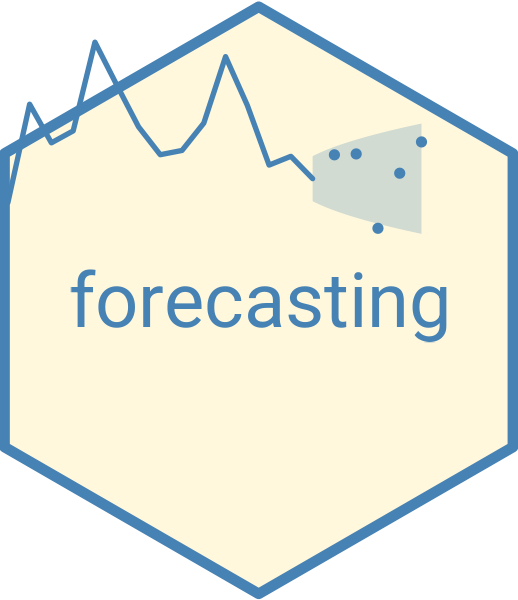
\includegraphics{forecasting-logo.png}\LARGE\\}
\posttitle{\end{center}}
\ifluatex
  \usepackage{selnolig}  % disable illegal ligatures
\fi

\title{Introduction to Time Series Modeling and Forecasting with Applications in R}
\author{David Ubilava}
\date{April 2022}

\begin{document}
\maketitle

{
\setcounter{tocdepth}{1}
\tableofcontents
}
\hypertarget{foreword}{%
\chapter*{Foreword}\label{foreword}}
\addcontentsline{toc}{chapter}{Foreword}

`Prediction is very difficult, especially about the future.' -- a perfect quote about our inability to make a perfect forecast, often attributed to Niels Bohr, is very much on-brand for the study of forecasting. And so it goes.

I came across this quote as I was wrapping up my doctoral dissertation at Purdue University. My dissertation topic was `Nonlinear Multivariate Modeling and Forecasting of Commodity Prices.' When I started my doctoral degree, I had not taken a designated time series econometrics or forecasting course. By the time I was completing my degree, I had learned enough to know how difficult it was to achieve accurate forecasts. A chapter of my dissertation, which pretty much was a forecasting exercise, yielded the so-called `null results.' I felt uneasy about it. I had an urge to justify, somehow, these null results. And then I stumbled across this quote, which `saved my day.' I stuck it as an epigraph of my dissertation. It captured my struggles as a forecaster, and provided the context to the results of my work.

Some years later, as I started teaching a course on forecasting, I spend a great deal of time explaining---indeed preparing students for the inevitable---that forecasting is difficult, and that more often than not we will not be able to give accurate forecasts. But I also stress that this should not discourage us from trying because most great achievements in this world have myriads of failed attempts as a foundation.

What is forecast if not a guess? An educated guess, nonetheless. A good guess doesn't have to be spot-on. It almost never is, only if by fluke. In fact, an inaccurate guess can be helpful too. That we were unable to exactly predict an event, tells us something about the underlying processes that result in an outcome different from what we predicted. Such conjecture can be useful. Forecasting, even if inaccurate, can be useful. George Box's `all models are wrong but some are useful' is certainly suitable to the study of forecasting. This book introduces time series models and presents a case of their usefulness in predicting events.

\hypertarget{preliminaries}{%
\chapter*{Preliminaries}\label{preliminaries}}
\addcontentsline{toc}{chapter}{Preliminaries}

\hypertarget{introduction-to-forecasting}{%
\chapter{Introduction to Forecasting}\label{introduction-to-forecasting}}

Roots of forecasting extend very much to the beginning of human history. In their desire to predict the future, people have attempted to make forecasts of their own, or have used services of others. Fortunetellers, for example, have been forecast experts of some sort, basing their predictions on magic. They are less common in the current age. Astrologers, who rely on astronomical phenomena to foresee the future, maintain their relevance to this date. Over time, and particularly with the development of the study of econometrics, more rigorous forecasting methods have been introduced and developed. All methods -- primitive or complex, spurious or scientifically substantiated -- have one thing in common: they all rely (or, at least, pretend to rely) on \emph{information}.

Information is key in forecasting. It comes in many forms, but once it is organized and stored, we end up with \emph{data}. Data that is organized and stored a certain way -- chronologically and at regular intervals -- are referred to as the \emph{time series}. A diverse set of forecasting methods typically rely on insights from econometric analysis of time series. In time series analysis, the implied assumption is that the past tends to repeat itself, at least to some extent. So, if we well study the past, we \emph{may} be able to forecast an event with some degree of accuracy.

Accurate forecasting is difficult. Indeed, forecasting is difficult. So, as we forecast, we are bound to make mistakes, which manifest into the \emph{forecast errors}. We have these errors because we don't know the true model, so we make a guess about the most suitable model for time series analysis. We also have the errors because we don't know the true parameters of the model. Instead, using a subset of history we estimate the parameters, which are prone to a sampling error. Finally, even if our guess about the model is exactly correct, and even if our parameter estimates happen to be exactly equal to the true parameters of the `right' model, our forecasts may still be off, because of all those factors that have never happened in past, and only characterize the future. And because of this, there is no such thing as precise forecast, even if by fluke we were to exactly predict an outcome of an event. But some forecasts are better than others. And in search of such forecasts the study of time series econometrics has evolved.

\hypertarget{basics-of-time-series-econometics}{%
\chapter{Basics of Time Series Econometics}\label{basics-of-time-series-econometics}}

A time series is a realization of a sequence of random variables that are stored chronologically. This sequence is referred to as the \emph{stochastic process}. Thus, a time series is a realization of the stochastic process. We index time periods as \(1,2,\ldots,T\), so that the stochastic process is given by \(\{Y_t:t=1,\ldots,T\}\). A time series is represented by a set of observations: \(\{y_1,\ldots,y_T\}\). One can view a time series as a finite sample from an underlying doubly--infinite sequence: \(\{\ldots,y_{-1},y_{0},y_1,y_2,\ldots,y_T,y_{T+1},y_{T+2},\ldots\}\). This is to say that the history extends beyond the starting and ending time periods of the sample at hand.

\hypertarget{stationarity}{%
\section{Stationarity}\label{stationarity}}

If all random variables, from where the time series are drawn, have the same distribution, then we refer to such data as \emph{stationary} time series. Stationarity is an important feature, and the assumption, on which the time series analysis heavily relies.

Before diving any further into the concepts and methods of time series econometrics, consider the simplest kind of time series comprised of realizations from independent and identically distributed normal random variable with zero mean and constant variance: \(\varepsilon_t \sim iid\left(0,\sigma^2\right)\). The following graph plots this time series against time.

\begin{figure}
\centering
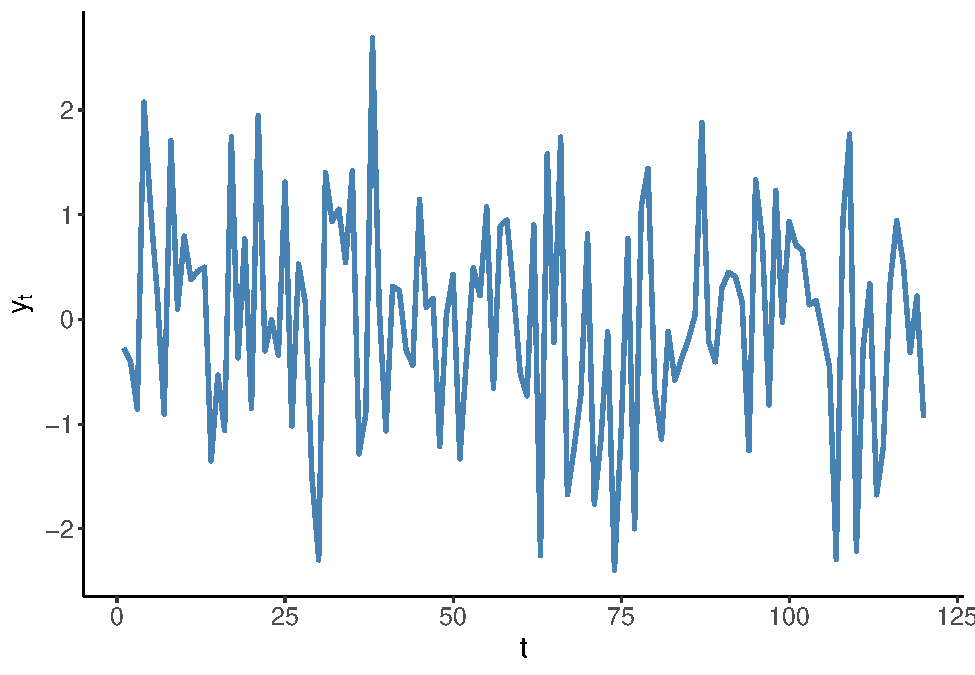
\includegraphics{forecasting_files/figure-latex/white-noise-1.pdf}
\caption{\label{fig:white-noise}White noise: an illustration}
\end{figure}

Such time series are referred to as \emph{white noise}. That is, \(\{y_t: t=1,\ldots,T\}\), is a white noise process if:
\begin{align*}
& E(y_t) = 0,\;~\forall~t\\
& Var(y_t) = \sigma^2,\;~\forall~t\\
& Cov(y_t,y_{t-k}) = 0,\;~\forall~k \ne 0
\end{align*}

Because each observation is drawn from the same distribution, white noise is a stationary time series. Indeed, it is a special type of stationary time series insofar as its mean, variance, and covariance are time-invariant. Note, for a time series to be stationary, neither the mean nor the covariances need to be equal to zero. Thus, \(\{y_t\}\) is stationary if the mean and variance are independent of \(t\), and the autocovariances are independent of \(t\) for all \(k\).

\hypertarget{serial-dependence}{%
\section{Serial Dependence}\label{serial-dependence}}

It is more of the norm rather than the exception for a time series to be correlated over time. Indeed, because of the sequential nature of time series, we commonly observe dependence among the temporally adjacent time series. That is, for most economic time series, we would expect \(y_t\) and \(y_{t-1}\) to be correlated. Such correlation, referred to as the first order \emph{autocorrelations}, is given by: \(\rho_1=Cor(y_{t},y_{t-1}) = \frac{Cov(y_{t},y_{t-k})}{Var(y_t)}\). In general, the \(k^{th}\) order autocorrelation is given by: \[\rho_k=Cor(y_{t},y_{t-k}) = \frac{Cov(y_{t},y_{t-k})}{Var(y_{t})},\;~~k=1,2,\ldots\]

Autocorrelations are commonly illustrated via the so-called \emph{autocorrelogram}, which plots the sequence of autocorrelation coefficients against the lags at which these coefficients are obtained. For example, an autocorrelogram of the previously illustrated white noise process is as follows:

\begin{figure}
\centering
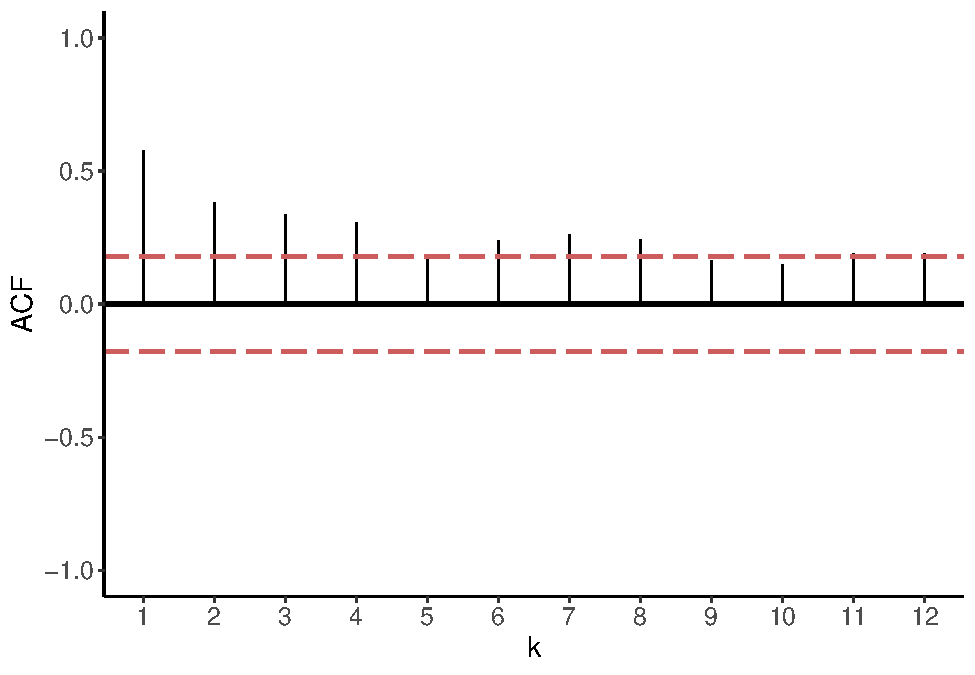
\includegraphics{forecasting_files/figure-latex/acf-1.pdf}
\caption{\label{fig:acf}Autocorrelation}
\end{figure}

For each \(k\), the vertical line extending from zero represents the autocorrelation coefficient at that lag. The red dashed lines denote the 90\% confidence interval, given by \(\pm 1.96/\sqrt{T}\), where \(T\) is the length of the time series.

Another relevant measure of the time series dependence is partial autocorrelation, which is correlation between \(y_t\) and \(y_{t-k}\) net of any correlations between \(y_t\) and \(y_{t-k+j}\), for all \(j=1,\ldots,k-1\). Similar to autocorrelations, partial autocorrelations can also be illustrated using autocorrelograms:

\begin{figure}
\centering
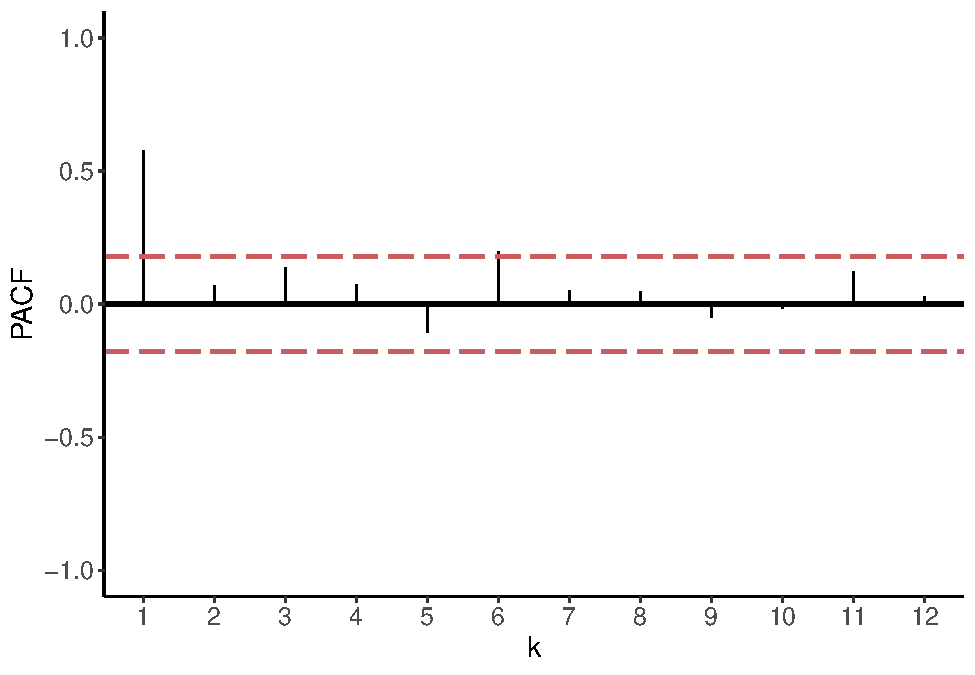
\includegraphics{forecasting_files/figure-latex/pacf-1.pdf}
\caption{\label{fig:pacf}Partial Autocorrelation}
\end{figure}

\begin{figure}
\centering
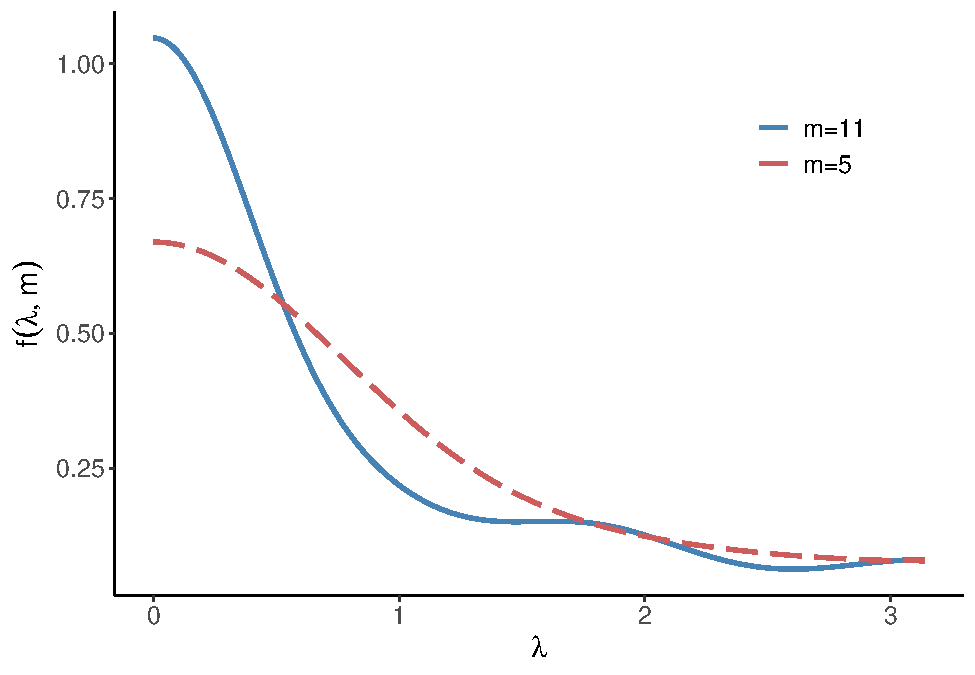
\includegraphics{forecasting_files/figure-latex/spectral-1.pdf}
\caption{\label{fig:spectral}Spectral Density}
\end{figure}

\hypertarget{transformations}{%
\section{Transformations}\label{transformations}}

It is common to transform time series by taking logarithms, differences, or differences of logarithms (growth rates). Such transformations usually are done to work with the suitable variable for the desired econometric analysis. For example, if an economic time series is characterized by an apparent exponential growth (e.g., real GDP), by taking natural logarithms the time series ``flatten'\,' and the fluctuations become proportionate. The difference operator is denoted by \(\Delta\), so that \(\Delta y_t = y_t-y_{t-1}\). The following three graphs illustrate (i) a time series with an apparent exponential growth, (ii) the natural logarithm of this time series, and (iii) their differences (i.e., the log-differences of the original series).

\begin{figure}
\centering
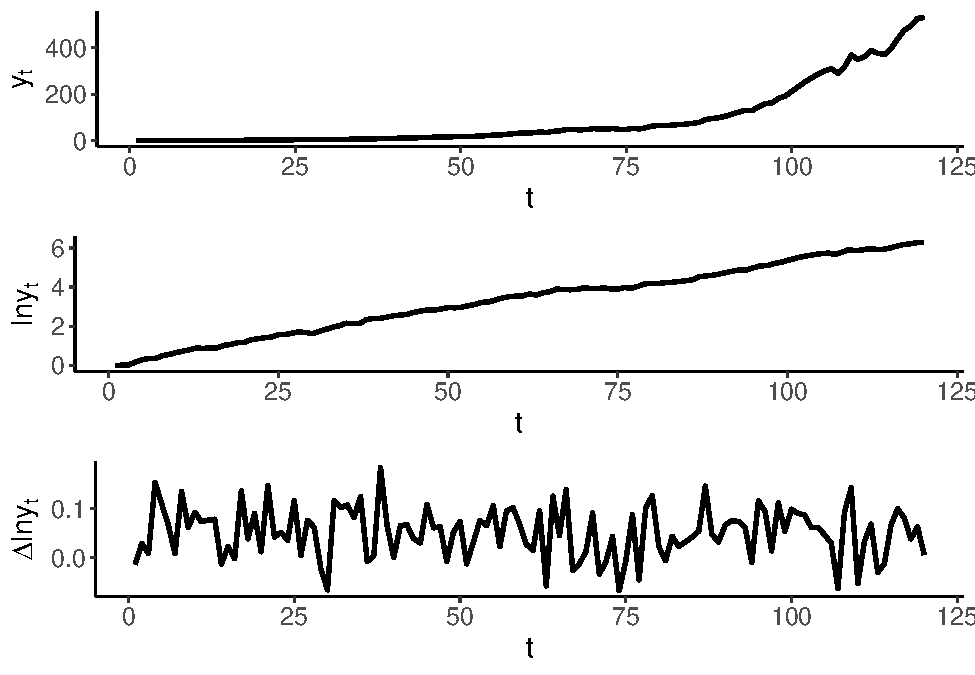
\includegraphics{forecasting_files/figure-latex/ts-1.pdf}
\caption{\label{fig:ts}A time series and its transformations}
\end{figure}

\hypertarget{forecasting-methods-and-routines}{%
\chapter{Forecasting Methods and Routines}\label{forecasting-methods-and-routines}}

\hypertarget{optimal-forecast}{%
\section{Optimal Forecast}\label{optimal-forecast}}

A forecast is a random variable which has some distribution and, thus, moments. The simplest form of a forecast is a point forecast (usually a mean of the distribution, but can be a median or, indeed, any quantile).

A point forecast made in period \(t\) for horizon \(h\) can be denoted as \(y_{t+h|t}\); this is our `best guess,' that is made in period \(t\), about the actual realization of the random variable in period \(t+h\), denoted by \(y_{t+h}\). The difference between the two is the forecast error. That is, \[e_{t+h|t} = y_{t+h} - y_{t+h|t}\]

The more accurate is the forecast the smaller is the forecast error.

Three types of uncertainty contribute to the forecast error:
\[\begin{aligned}
        e_{t+h|t} & = \big[y_{t+h}-E(y_{t+h}|\Omega_{t})\big]\;~~\text{(forecast uncertainty)}  \\
        & + \big[E(y_{t+h}|\Omega_{t}) - g(\Omega_{t};\theta)\big]\;~~\text{(model uncertainty)}  \\
        & + \big[g(\Omega_{t};\theta)-g(\Omega_{t};\hat{\theta})\big]\;~~\text{(parameter uncertainty)}
        \end{aligned}\]

where \(\Omega_t\) denotes the information set available at the time when the forecast is made; \(g(\cdot)\) is a functional form of a model applied to the data; \(\theta\) is a set of parameters of the model, and \(\hat{\theta}\) are their estimates

Because uncertainty cannot be avoided, a forecaster is bound to commit forecast errors. The goal of the forecaster is to minimize the `cost' associated with the forecast errors. This is achieved by minimizing the expected loss function.

A loss function, \(L(e_{t+h|t})\), can take many different forms, but is should satisfy the following properties:
\[\begin{aligned}
        & L(e_{t+h|t}) = 0,\;~~\forall\;e_{t+h|t} = 0 \\
        & L(e_{t+h|t}) \geq 0,\;~~\forall\;e_{t+h|t} \neq 0 \\
        & L(e_{t+h|t}^{(i)}) > L(e_{t+h|t}^{(j)}),\;~~\forall\;|e_{t+h|t}^{(i)}| > |e_{t+h|t}^{(j)}|
        \end{aligned}\]

Two commonly used symmetric loss functions are \emph{absolute} and \emph{quadratic} loss functions:
\[\begin{aligned}
        & L{(e_{t+h|t})} = |e_{t+h|t}|\;~~\text{(absolute loss function)} \\
        & L{(e_{t+h|t})} = (e_{t+h|t})^2\;~~\text{(quadratic loss function)}
        \end{aligned}\]

The quadratic loss function is popular, partly because we typically select models based on `in-sample' quadratic loss (i.e.~by minimizing the sum of squared residuals).

Optimal forecast is the forecast that minimizes the expected loss:
\[\min_{y_{t+h|t}} E\left[L\left(e_{t+h|t}\right)\right] = \min_{y_{t+h|t}} E\left[L\left(y_{t+h}-y_{t+h|t}\right)\right]\]
where the expected loss is given by:
\[E\left[L\left(y_{t+h}-y_{t+h|t}\right)\right]=\int L\left(y_{t+h}-y_{t+h|t}\right) f(y_{t+h}|\Omega_t)dy\]

We can assume that the conditional density is a normal density with mean \(\mu_{t+h} \equiv E(y_{t+h})\), and variance \(\sigma_{t+h}^2 \equiv Var(y_{t+h})\).

Under the assumption of the quadratic loss function:
\[\begin{aligned}
        E\left[L(e_{t+h|t})\right] & = E(e_{t+h|t}^2) = E(y_{t+h} - \hat{y}_{t+h|t})^2 \\
        & = E(y_{t+h}^2)-2E(y_{t+h})\hat{y}_{t+h|t} + \hat{y}_{t+h|t}^2
        \end{aligned}\]

By solving the optimization problem it follows that: \[\hat{y}_{t+h|t} = E(y_{t+h}) \equiv \mu_{t+h}\]

Thus, the optimal point forecast under the quadratic loss is the \emph{mean} (for reference, the optimal point forecast under absolute loss is the \emph{median}).

\hypertarget{measuring-forecast-accuracy}{%
\section{Measuring Forecast Accuracy}\label{measuring-forecast-accuracy}}

Forecast accuracy should only be determined by considering how well a model performs on data not used in estimation. But to assess forecast accuracy we need access to the data, typically from future time periods, that was not used in estimation. This leads to the so-called `pseudo forecasting' routine. This routine involves splitting the available data into two segments referred to as `in-sample' and `out-of-sample.' The in-sample segment of a series is also known as the `estimation set' or the `training set.' The out-of-sample segment of a series is also known as the `hold-out set' or the `test set.'

Thus, we make the so-called `genuine' forecasts using only the information from the estimation set, and assess the accuracy of these forecasts in an out-of-sample setting.

Because forecasting is often performed in a time series context, the estimation set typically predates the hold-out set. In non-dynamic settings such chronological ordering may not be necessary, however.

There are different forecasting schemes for updating the information set in the pseudo-forecasting routine. These are: \emph{recursive}, \emph{rolling}, and \emph{fixed}.

\begin{itemize}
\tightlist
\item
  The recursive forecasting environment uses a sequence of expanding windows to update model estimates and the information set.
\item
  The rolling forecasting environment uses a sequence of rolling windows of the same size to update model estimates and the information set.
\item
  The fixed forecasting environment uses one fixed window for model estimates, and only updates the information set.
\end{itemize}

The following animation illustrates the distinctive features of these three routines:

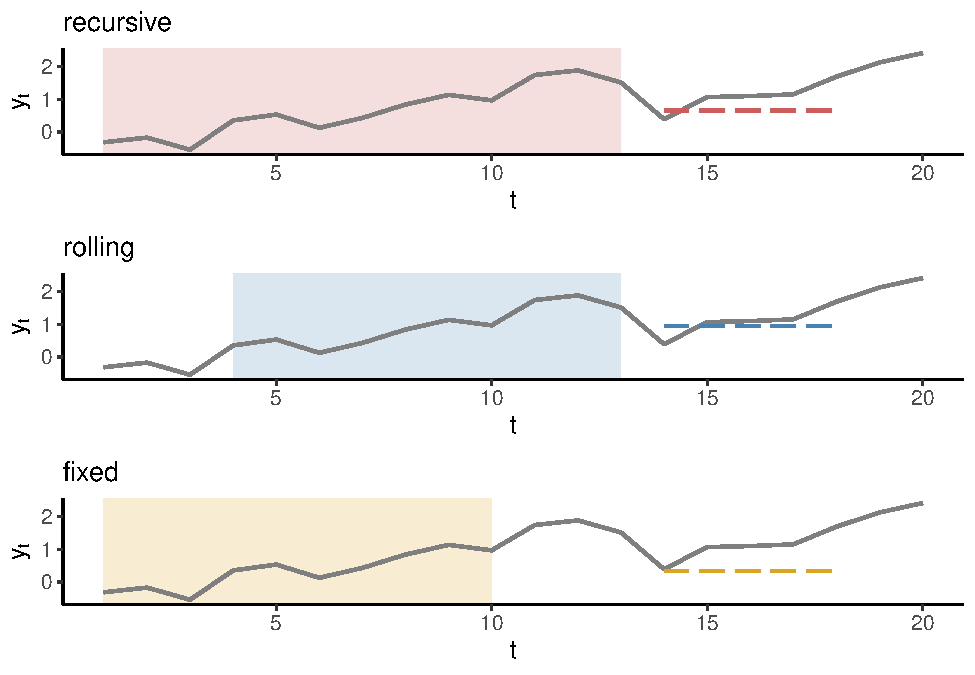
\includegraphics{forecasting_files/figure-latex/routines-1.pdf}

\hypertarget{evaluating-time-series-forecasts}{%
\section{Evaluating Time Series Forecasts}\label{evaluating-time-series-forecasts}}

To evaluate forecasts of a time series, \(\{y_t\}\), with a total of \(T\) observations, we divide the sample into two parts, the in-sample set with a total of \(R\) observations, such that \(R < T\) (typically, \(R \approx 0.75T\)), and the out-of-sample set.

For example, if we are interested in one-step-ahead forecast assessment, this way we will produce a sequence of forecasts: \(\{y_{R+1|R},y_{R+2|{R+1}},\ldots,y_{T|{T-1}}\}\) for \(\{Y_{R+1},Y_{R+2},\ldots,Y_{T}\}\).

Forecast errors, \(e_{R+j} = y_{R+j} - y_{R+j|{R+j-1}}\), then can be computed for \(j = 1,\ldots,T-R\).

The most commonly applied accuracy measures are the mean absolute forecast error (MAFE) and the root mean squared forecast error (RMSFE):
\[\begin{aligned}
\text{MAFE}  = & \frac{1}{P}\sum_{i=1}^{P}|e_i|\\
\text{RMSFE} = & \sqrt{\frac{1}{P}\sum_{i=1}^{P}e_i^2}
\end{aligned}\]
where \(P\) is the total number of out-of-sample forecasts. The lower is the accuracy measure (of choice), the better a given model performs in generating accurate forecasts. As noted earlier, `better' does not mean `without errors.'

Forecast errors of a `good' forecasting method will have the following properties:

\begin{itemize}
\tightlist
\item
  zero mean; otherwise, the forecasts are biased.
\item
  no correlation with the forecasts; otherwise, there is information left that should be used in computing forecasts.
\item
  no serial correlation among one-step-ahead forecast errors. Note that \(k\)-step-ahead forecasts, for \(k>1\), can be, and usually are, serially correlated.
\end{itemize}

Any forecasting method that does not satisfy these properties has a potential to be improved.

\hypertarget{unbiasedness}{%
\subsection{Unbiasedness}\label{unbiasedness}}

Testing \(E(e_{t+h|t})=0\). Set up a regression: \[e_{t+h|t} = \alpha+\upsilon_{t+h} \hspace{.5in} t = R,\ldots,T-h,\]
where \(R\) is the estimation window size, \(T\) is the sample size, and \(h\) is the forecast horizon length. The null of zero-mean forecast error is equivalent of testing \(H_0: \alpha = 0\) in the OLS setting. For \(h\)-step-ahead forecast errors, when \(h>1\), autocorrelation consistent standard errors should be used.

\hypertarget{efficiency}{%
\subsection{Efficiency}\label{efficiency}}

Testing \(Cov(e_{t+h|t},y_{t+h|t})=0\). Set up a regression: \[e_{t+h|t} = \alpha + \beta y_{t+h|t} + \upsilon_{t+h} \hspace{.5in} t = R,\ldots,T-h.\] The null of forecast error independence of the information set is equivalent of testing \(H_0: \beta = 0\) in the OLS setting. For \(h\)-step-ahead forecast errors, when \(h>1\), autocorrelation consistent standard errors should be used.

\hypertarget{no-autocorrelation}{%
\subsection{No Autocorrelation}\label{no-autocorrelation}}

Testing \(Cov(e_{t+1|t},e_{t|t-1})=0\). Set up a regression: \[e_{t+1|t} = \alpha + \gamma e_{t|t-1} + \upsilon_{t+1} \hspace{.5in} t = R+1,\ldots,T-1.\] The null of no forecast error autocorrelation is equivalent of testing \(H_0: \gamma = 0\) in the OLS setting.

\hypertarget{deterministic-time-series-models}{%
\chapter*{Deterministic Time Series Models}\label{deterministic-time-series-models}}
\addcontentsline{toc}{chapter}{Deterministic Time Series Models}

\hypertarget{trends}{%
\chapter{Trends}\label{trends}}

Economic time series usually are characterized by trending behavior, and often present a seasonal pattern as well. Trend is a unidirectional change of time series over an extended period of time that arises from the accumulation of information over time. Seasonality is a repeating pattern \emph{within a calendar year} that arises from the links of technologies, preferences, and institutions to the calendar. Modeling and forecasting these time series features is a fairly straightforward task. But before we get to it, let's discuss what may happen if we were to ignore the presence of trends and/or seasonality when analyzing the time series data.

\hypertarget{spurious-relationship}{%
\section{Spurious Relationship}\label{spurious-relationship}}

Nothing about trending time series necessarily violates the classical linear regression model assumptions. The issue may arise, however, if an unobserved trending variable is simultaneously correlated with the dependent variable as well as one of the independent variables in a time series regression. In such case, we may find a (statistically significant) relationship between two or more unrelated economic variables simply because they are all trending. Such relationship is referred to a \emph{spurious relationship}.

To illustrate, consider two trending variables: \[y_t = \gamma t + \nu_t,\;~~\nu\sim N(0,\sigma_{\nu}^2),\] and \[x_t = \delta t + \upsilon_t,\;~~\upsilon\sim N(0,\sigma_{\upsilon}^2),\] where \(Cov(\nu_t,\upsilon_t) = 0\). For simplicity, we can assume \(\sigma_{\nu}^2=\sigma_{\upsilon}^2=1\). Suppose, \(\gamma\) and \(\delta\) are some positive scalars, say, \(0.3\) and \(0.5\), respectively. That is, \(y\) and \(x\) are trending in the same direction. Below is an example of such time series:
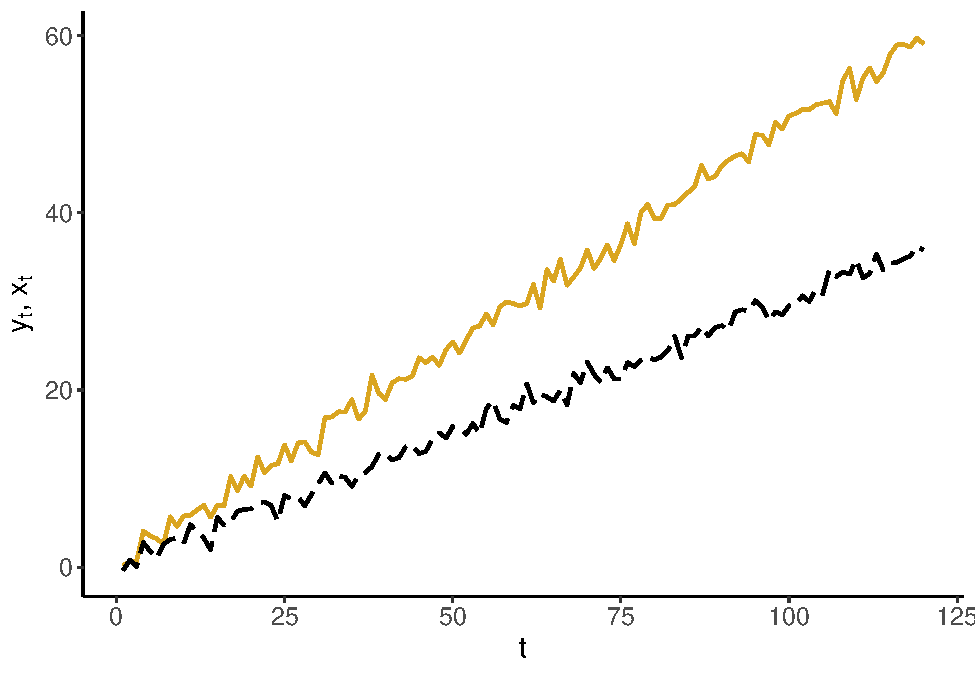
\includegraphics{forecasting_files/figure-latex/unnamed-chunk-6-1.pdf}

If we were to estimate \[y_t = \alpha+\beta x_t + \varepsilon_t,\] we are likely to find the relationship between the two -- in this case \(\beta>0\) -- even though, we know, the two are not related. To illustrate this, we will generate 1000 samples of size 120 for \(y\) and \(x\), and in each case we will estimate the parameter \(\beta\). The following graph illustrates the empirical distribution of these parameter estimates:
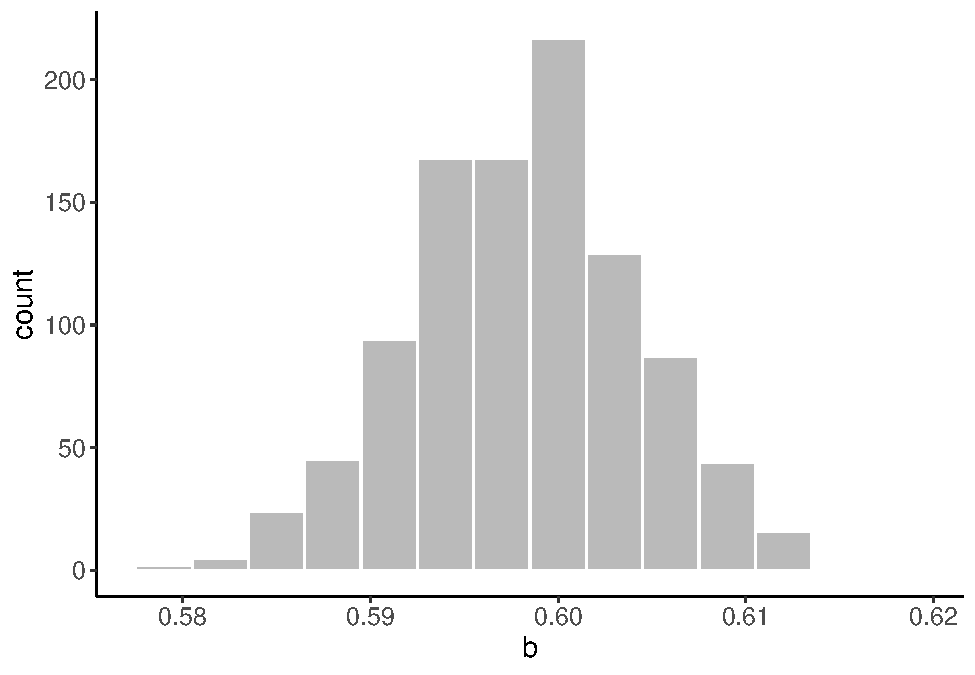
\includegraphics{forecasting_files/figure-latex/unnamed-chunk-7-1.pdf}

Luckily, we can easily ``fix'' the issue, by incorporating a trend in the regression: \[y_t = \alpha+\beta x_t + \eta t + \varepsilon_t.\] Once the trend is accounted for, the previously illustrated ``bias'' disappears. Using a similar simulation exercise as before, the following graph illustrates the empirical distribution of these parameter estimates:
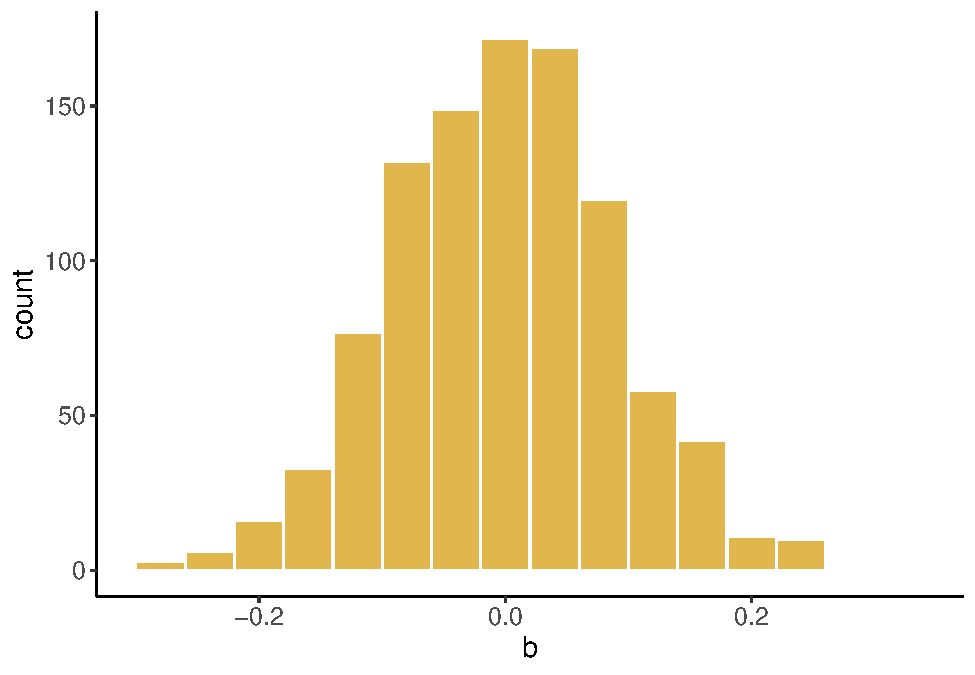
\includegraphics{forecasting_files/figure-latex/unnamed-chunk-8-1.pdf}

In fact, this ``fix'' is equivalent to regressing a de-trended \(y\) on a de-trended \(x\). To de-trend a variable, we first run a regression: \(y_t = \gamma_0 + \gamma_1 t + \nu_t\), and then obtain the fitted values for some fixed trend (typically zero), that is: \(\tilde{y}_t = \hat{\gamma}_0+\hat{\nu}_t\), where \(\hat{\gamma}_0\) and \(\hat{\nu}_t\) are the parameter estimate and the residuals from the foregoing regression.

\hypertarget{modeling}{%
\section{Modeling}\label{modeling}}

As seen, accounting for trends in a time series can help us resolve some regression issues. But a trend in and of itself can be an inherent feature of a times series. To that end, we can apply deterministic trends to forecast time series.

The simplest (and perhaps most frequently applied) model to account for the trending time series is a \emph{linear} trend model: \[y_t = \alpha + \beta t\]

Other likely candidate trend specifications are \emph{polynomial} (e.g.~quadratic, cubic, etc.), \emph{exponential}, and \emph{shifting} (or \emph{switching}) trend models, respectively given by:
\[\begin{aligned}
    y_t &= \alpha + \beta_1 t + \beta_2 t^2 + \ldots + \beta_p t^p \\
    y_t &= e^{\alpha + \beta t}\;~~\mbox{or}\;~~\ln{y_t} = \alpha + \beta t \\
    y_t &= \alpha + \beta_1 t + \beta_2 (t-\tau)I(t>\tau),\;~~\tau\in\mathsf{T} 
    \end{aligned}\]

Of these, here we will primarily consider linear and quadratic trends. An exponential trend, from the standpoint of modeling and forecasting, is equivalent to a linear trend fitted to natural logarithm of the series. For a time series \(\{y_t: t=1,\ldots,T\}\), the natural logarithm is: \(z_t = \ln{y_t}\). Some of the benefits of such a transformation are that:

\begin{itemize}
\tightlist
\item
  they are easier to interpret (relative/percentage change).
\item
  they homogenizes the variance of the time series.
\item
  they may result in improved forecasting accuracy.
\end{itemize}

Exponential trends are suitable when a time series is characterized by a stable relative change over time (e.g., when economic time series grow by 2\% every year).

We will cover the shifting/switching trend models in another chapter.

Trends are (relatively) easy to model and forecast. Caution is needed, however, with (higher order) polynomial trends, as they may fit well in-sample, but cause major problems out-of-sample.

Consider a linear trend model with an additive error term: \[y_t = \alpha + \beta t + \varepsilon_t\] We estimate the model parameters, \(\mathbf{\theta}=\{\alpha,\beta\}\), by fitting the trend model to a time series using the least-squares regression: \[\hat{\theta} = \operatorname*{argmin}_{\mathbf{\theta}} \sum_{t=1}^{T}\big(y_t - \alpha - \beta t\big)^2.\] Fitted values are then given by: \[\hat{y}_t = \hat{\alpha} + \hat{\beta} t\]

\hypertarget{forecasting}{%
\section{Forecasting}\label{forecasting}}

If a linear trend model is fitted to the data, then any future realization of the stochastic process is assumed to follow the linear trend model: \[y_{t+h} = \alpha + \beta (t+h) + \varepsilon_{t+h}.\]

An optimal forecast of \(y_{t+h}\), therefore, is given by: \[y_{t+h|t} = E(y_{t+h}|\Omega_t) = E[\alpha + \beta (t+h) + \varepsilon_{t+h}] = \alpha + \beta (t+h).\]

The forecast error is: \[e_{t+h|t} = y_{t+h} - y_{t+h|t} = \varepsilon_{t+h}\]

The forecast variance, then, is: \[\sigma_{t+h|t}^2 = E(e_{t+h|t}^2) =  E(\varepsilon_{t+h}^2) = \hat{\sigma}^2,\;~~\forall\;h\]

From this, we can obtain interval forecast at any horizon, which is: \[y_{t+h|t} \pm 1.96 \hat{\sigma}.\]

A few features of trend forecasts to note:

\begin{itemize}
\tightlist
\item
  they tend to understate uncertainty (at long horizons as the forecast interval doesn not widen with the horizon);
\item
  short-term trend forecasts can perform poorly; long-term trend forecasts typically perform poorly;
\item
  sometimes it may be beneficial, from the standpoint of achieving better accuracy, to forecast growth rates, and then reconstruct level forecasts.
\end{itemize}

\hypertarget{seasonality}{%
\chapter{Seasonality}\label{seasonality}}

Seasonality is typically modeled as monthly or quarterly pattern, but can also be modeled as a higher frequency pattern (e.g.~weekly). Some examples of time series with apparent seasonal patterns are:

\begin{itemize}
\tightlist
\item
  Agricultural production.
\item
  Sales of energy products.
\item
  Airfare (in non-pandemic times).
\end{itemize}

One way to deal with the seasonality in data is to ``remove'' it prior to the use of the series (i.e., work with a seasonally adjusted time series). Indeed, some economic time series are only/also available in a seasonally-adjusted form.

Otherwise, and perhaps more interestingly, we can directly model seasonality in a regression setting by incorporating seasonal dummy variables, for example.

\hypertarget{modeling-1}{%
\section{Modeling}\label{modeling-1}}

A seasonal model is given by: \[y_t = \sum_{i=1}^{s}\gamma_i d_{it} + \varepsilon_t,\]
where \(s\) denotes the frequency of the data, and \(d_{it}\) takes the value of 1 repeatedly after every \(s\) periods, and such that \(\sum_{i} d_{it} = 1\), \(\forall t\).

Alternatively the seasonal model can be rewritten as: \[y_t = \alpha + \sum_{i=1}^{s-1}\delta_i d_{it} + \varepsilon_t,\] in which case \(\alpha\) is an intercept of an omitted season, and \(\delta_i\) represents a deviation from it during the \(i^{th}\) season. This is a more typical form of a seasonal model.

Both variants of a seasonal model result in an identical fit and forecasts.

When dealing with weekly or daily data, the dummy variable approach of modeling seasonality may not be practical, nor efficient in most instances, as that will require estimating another 51 or 364 parameters. A way to model seasonality without giving up too many degrees of freedom is by using the so-called harmonic seasonal variables, which are a set of Fourier terms.

The Fourier terms can be applied to model seasonality at any frequency, indeed. Suppose, for example, we are working with monthly time series. A model with Fourier terms will have the following form: \[y_t = \alpha+\sum_{k=1}^{K}\left[\beta_{1k}\sin\left(\frac{2\pi kt}{12}\right)+\beta_{2k}\cos\left(\frac{2\pi kt}{12}\right)\right]+\varepsilon_t,\] where the value of \(K\) can be determined using an information criterion (e.g., AIC or SIC).

\hypertarget{forecasting-1}{%
\section{Forecasting}\label{forecasting-1}}

The predictors of the seasonal models are pre-determined, which means, after fitting the model, we can directly obtain the point and interval forecasts for any horizon \(h\).

When using the dummy variable approach to model the seasonality, for example, a future realization of a random variable is: \[y_{t+h} = \alpha + \sum_{i=1}^{s-1}\delta_i d_{i,t+h} + \varepsilon_{t+h}.\]

The optimal forecast of \(y_{t+h}\) is: \[y_{t+h|t} = E(y_{t+h}|\Omega_t) = \alpha + \sum_{i=1}^{s-1}\delta_i d_{i,t+h}\]

The forecast error is: \[e_{t+h|t} = y_{t+h} - y_{t+h|t} = \varepsilon_{t+h}\]

The forecast variance is: \[\sigma_{t+h|t}^2 = E(e_{t+h|t}^2) =  E(\varepsilon_{t+h}^2) = \hat{\sigma}^2,\;~~\forall\;h\]

The interval forecast is: \[y_{t+h|t} \pm 1.96 \hat{\sigma}.\]

\hypertarget{dynamic-time-series-models}{%
\chapter*{Dynamic Time Series Models}\label{dynamic-time-series-models}}
\addcontentsline{toc}{chapter}{Dynamic Time Series Models}

\hypertarget{linear-autoregression}{%
\chapter{Linear Autoregression}\label{linear-autoregression}}

Economic time series are often characterized by stochastic cycles. A cycle is a pattern of periodic fluctuations, not contained within a calendar year. A stochastic cycle is one generated by random variables. In general terms, the process is given by:
\[Y_t = f(Y_{t-1},Y_{t-2},\ldots;\mathbf{\theta})+\varepsilon_t.\;~~t=1,\ldots,T\]

An autoregressive process (or, simply, an autoregression) is a regression in which the dependent variable and the regressors belong to the same stochastic process.

An autoregression of order \(p\), denoted as \(AR(p)\), has the following functional form:
\[y_t = \alpha + \beta_1 y_{t-1}+\beta_2 y_{t-2}+ \cdots + \beta_p y_{t-p}+\varepsilon_t\]

The sum of the autoregressive parameters, \(\beta_1,\ldots,\beta_p\), depicts the persistence of the series. The larger is the persistence (i.e., closer it is to one), the longer it takes for the effect of a shock to dissolve. The effect will, eventually, dissolve so long as the series are covariance-stationary.

The autocorrelation, \(\rho\), and partial autocorrelation, \(\pi\), functions of the covariance-stationary \(AR(p)\) process have the following distinctive features:

\begin{itemize}
\tightlist
\item
  \(\rho_1 = \pi_1\), and \(\pi_p = \beta_p\).
\item
  The values of \(\beta_1,\ldots,\beta_p\) determine the shape of the autocorrelation function (ACF); in any case, the smaller (in absolute terms) is the persistence measure, the faster the ACF decays toward zero.
\item
  The partial autocorrelation function (PACF) is characterized by ``statistically significant'' first \(p\) spikes \(\pi_1 \neq 0,\ldots,\pi_p \neq 0\), and the remaining \(\pi_k = 0\), \(\forall k > p\).
\end{itemize}

\hypertarget{modeling-2}{%
\section{Modeling}\label{modeling-2}}

\hypertarget{ar1}{%
\subsection{AR(1)}\label{ar1}}

The first-order autoregression is given by: \[y_t = \alpha + \beta_1 y_{t-1} + \varepsilon_t,\] where \(\alpha\) is a constant term; \(\beta_1\) is the \emph{persistence} parameter; and \(\varepsilon_t\) is a white noise process.

A necessary and sufficient condition for an \(AR(1)\) process to be covariance stationary is that \(|\beta_1| < 1\). We can see this by substituting recursively the lagged equations into the lagged dependent variables:
\[
\begin{aligned}
y_t &= \alpha + \beta_1 y_{t-1} + \varepsilon_t \notag \\
y_t &= \alpha + \beta_1 (\alpha + \beta_1 y_{t-2} + \varepsilon_{t-1}) + \varepsilon_t \notag \\
&= \alpha(1+\beta_1) + \beta_1^2 (\alpha + \beta_1 y_{t-3} + \varepsilon_{t-2}) + \beta_1\varepsilon_{t-1} + \varepsilon_t \notag \\
&\vdots  \notag \\
&= \alpha\sum_{i=0}^{k-1}\beta_1^i + \beta_1^k y_{t-k} + \sum_{i=0}^{k-1}\beta_1^i\varepsilon_{t-i}
\end{aligned}
\]
The end-result is a general linear process with geometrically declining coefficients. Here, \(|\beta_1| < 1\) is required for convergence.

Assuming \(|\beta_1| < 1\), as \(k \to \infty\) the process converges to: \[y_t = \frac{\alpha}{1-\beta_1} + \sum_{i=0}^{\infty}\beta_1^i\varepsilon_{t-i}\]

The \emph{unconditional mean} of this process is: \[\mu = E\left(y_t\right) = E\left(\frac{\alpha}{1-\beta_1} + \sum_{i=0}^{\infty}\beta_1^i\varepsilon_{t-i}\right) = \frac{\alpha}{1-\beta_1}\]

The \emph{unconditional variance} of this process is: \[\gamma_0 = Var\left(y_t\right) = Var\left(\frac{\alpha}{1-\beta_1} + \sum_{i=0}^{\infty}\beta_1^i\varepsilon_{t-i}\right) = \frac{\sigma_{\varepsilon}^2}{1-\beta_1^2}\]

The \emph{Autocovariance} is simply the covariance between \(y_t\) and \(y_{t-k}\), that is: \[\gamma_k = Cov(y_t,y_{t-k}) = E[(y_t - \mu)(y_{t-k} - \mu)] = E(y_t y_{t-k}) - \mu^2\]

Some algebraic manipulation can help us show that: \[\gamma_k = \beta_1\gamma_{k-1},\] and that: \[\rho_{k} = \beta_1\rho_{k-1}\] (recall, \(\rho_k = \gamma_k/\gamma_0\) is the autocorrelation coefficient).

In fact, for AR(1), an autocorrelation coefficient of some lag can be represented as the autoregression parameter (which in this instance is equivalent to the persistence measure) to that power. That is:
\[
\begin{aligned}
\rho_1 &= \beta_1\rho_0 = \beta_1 \notag \\
\rho_2 &= \beta_1\rho_1 = \beta_1^2 \notag \\
&\vdots \notag \\
\rho_k &= \beta_1\rho_{k-1} = \beta_1^k
\end{aligned}
\]

It follows that the autocorrelation function of a covariance stationary AR(1) is a geometric decay; the smaller is \(|\beta_1|\) the more rapid is the decay.

By imposing certain restrictions, the AR(1) will reduce to other already known models:

\begin{itemize}
\tightlist
\item
  If \(\beta_1 = 0\), \(y_t\) is equivalent to a white noise.
\item
  If \(\beta_1 = 1\) and \(\alpha = 0\), \(y_t\) is a random walk.
\item
  If \(\beta_1 = 1\) and \(\alpha \neq 0\), \(y_t\) is a random walk with drift.
\end{itemize}

In general, a smaller persistence parameter results in a quicker adjustment to the \emph{unconditional mean} of the process.

The autocorrelation and partial autocorrelation functions of the AR(1) process have three distinctive features:

\begin{itemize}
\tightlist
\item
  \(\rho_1 = \pi_1 = \beta_1\). That is, the persistence parameter is also the autocorrelation and the partial autocorrelation coefficient.
\item
  The autocorrelation function decreases exponentially toward zero, and the decay is faster when the persistence parameter is smaller.
\item
  The partial autocorrelation function is characterized by only one spike \(\pi_1 \neq 0\), and the remaining \(\pi_k = 0\), \(\forall k > 1\).
\end{itemize}

To illustrate the foregoing, let's generate a series of 100 observations that follow the process: \(y_t=0.8y_{t-1}+\varepsilon_t\), where \(y_0=0\) and \(\varepsilon\sim N(0,1)\), and plot the ACF and PACF of this series.

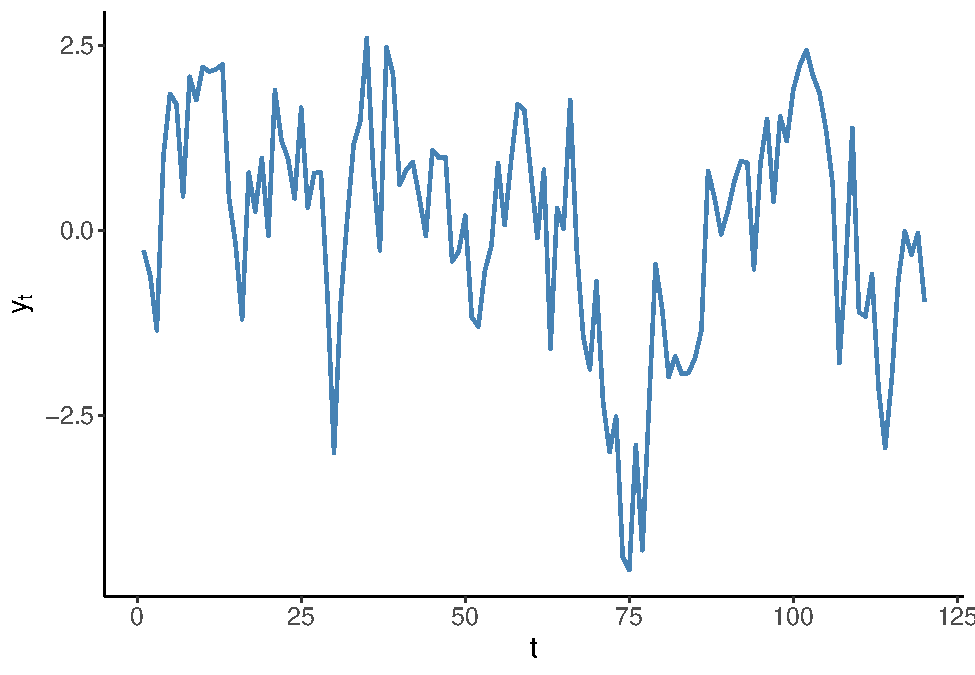
\includegraphics{forecasting_files/figure-latex/unnamed-chunk-11-1.pdf}

\hypertarget{ar2}{%
\subsection{AR(2)}\label{ar2}}

Now consider the second-order autoregression: \[y_t = \alpha + \beta_1 y_{t-1} + \beta_2 y_{t-2} + \varepsilon_t\]

where \(\alpha\) is a constant term; \(\beta_1+\beta_2\) is the persistence measure; and \(\varepsilon_t\) is a white noise process.

In what follows, the necessary (1 and 2) and sufficient (3 and 4) conditions for an \(AR(2)\) process to be covariance stationary are:

\begin{enumerate}
\def\labelenumi{\arabic{enumi}.}
\tightlist
\item
  \(|\beta_2| < 1\)
\item
  \(|\beta_1| < 2\)
\item
  \(\beta_1 + \beta_2 < 1\)
\item
  \(\beta_2 - \beta_1 < 1\)
\end{enumerate}

The autocorrelation functions of the AR(2) process have the following distinctive features:

\begin{itemize}
\tightlist
\item
  \(\rho_1 = \pi_1\) (which is true for any \(AR(p)\) process), and \(\pi_2 = \beta_2\).
\item
  The autocorrelation function decreases toward zero. The path, however, varies depending on the values of \(\beta_1\) and \(\beta_2\). Nonetheless, the decay is faster when the persistence measure is smaller.
\item
  The partial autocorrelation function is characterized by only two spikes \(\pi_1 \neq 0\) and \(\pi_2 \neq 0\), and the remaining \(\pi_k = 0\), \(\forall k > 2\).
\end{itemize}

Again, to illustrate, let's generate a series of 100 observations that follow the process: \(y_t=1.1y_{t-1}-0.4y_{t-2}+\varepsilon_t\), where \(y_{-1}=y_0=0\) and \(\varepsilon\sim N(0,1)\), and plot the ACF and PACF of this series.

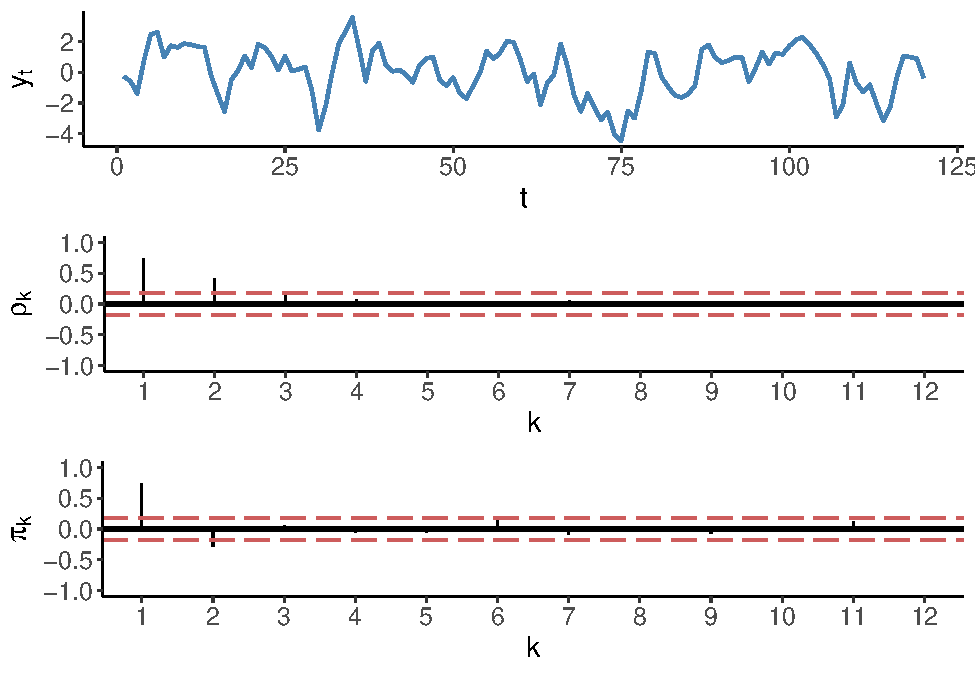
\includegraphics{forecasting_files/figure-latex/unnamed-chunk-12-1.pdf}

\hypertarget{forecasting-2}{%
\section{Forecasting}\label{forecasting-2}}

Making forecasts for some future period, \(t+h\), from an AR(p) model that has been fit to the data up to and including period \(t+h-1\) can be a straightforward exercise, so long as we have access to the relevant information set. For one-step-ahead forecasts, the information set is readily available. For multi-step-ahead forecasts, we need to `come up' with the value of the variable that has not been realized yet. For example, when making a two-step-ahead forecast for period \(t+2\), we need data from period \(t+1\), which is not available at the time when the forecast is made. Instead, we need to use our forecast for period \(t+1\). The same applies to forecasts for any subsequent periods in the future. This approach is known as an \emph{iterative} method of forecasting, wherein we make forecast for some period using the available data, then iterate forward by one period and use the most recent forecast to make the next period's forecast, and so on and so forth.

\hypertarget{one-step-ahead-forecast-from-ar1}{%
\subsection{One-step-ahead forecast from AR(1)}\label{one-step-ahead-forecast-from-ar1}}

The realization of the random variable in period \(t+1\) is: \[y_{t+1} = \alpha + \beta_1 y_{t} + \varepsilon_{t+1}\]

The optimal one-step-ahead forecast is: \[y_{t+1|t} = E(y_{t+1}|\Omega_t) = E(\alpha + \beta_1 y_{t} + \varepsilon_{t+1}) = \alpha + \beta_1 y_{t}\]

The one-step-ahead forecast error is: \[e_{t+1|t} = y_{t+1} - y_{t+1|t} = \alpha + \beta_1 y_t + \varepsilon_{t+1} - (\alpha + \beta_1 y_t) = \varepsilon_{t+1}\]

The one-step-ahead forecast variance: \[\sigma_{t+1|t}^2 = Var(y_{t+1}|\Omega_t) = E(e_{t+1|t}^2) = E(\varepsilon_{t+1}^2) = \sigma_{\varepsilon}^2\]

The one-step-ahead (95\%) interval forecast: \[y_{t+1|t} \pm z_{.025}\sigma_{t+1|t} = y_{t+1|t} \pm 1.96\sigma_{\varepsilon}\]

\hypertarget{two-step-ahead-forecast-from-ar1}{%
\subsection{Two-step-ahead forecast from AR(1)}\label{two-step-ahead-forecast-from-ar1}}

The realization of the random variable in period \(t+2\) is: \[y_{t+2} = \alpha + \beta_1 y_{t+1} + \varepsilon_{t+2}\]

The optimal two-step-ahead forecast is: \[y_{t+2|t} = E(y_{t+2}|\Omega_t) = E(\alpha + \beta_1 y_{t+1} + \varepsilon_{t+2}) = \alpha(1+\beta_1) + \beta_1^2 y_t\]

Note, that here we substituted \(y_{t+1}\) with \(\alpha + \beta_1 y_t + \varepsilon_{t+1}\).

The two-step-ahead forecast error is:
\[\begin{aligned}
e_{t+2|t} &= y_{t+2} - y_{t+2|t} \\
&= \alpha(1+\beta_1) + \beta_1^2 y_t + \beta_1\varepsilon_{t+1} + \varepsilon_{t+2} - [\alpha(1+\beta_1) + \beta_1^2 y_t] \\
&= \beta_1\varepsilon_{t+1} + \varepsilon_{t+2}
\end{aligned}\]

The two-step-ahead forecast variance is:
\[\begin{aligned}
\sigma_{t+2|t}^2 &= Var(y_{t+2}|\Omega_t) \\
&= E(e_{t+2|t}^2) = E(\beta_1\varepsilon_{t+1} + \varepsilon_{t+2})^2 = \sigma_{\varepsilon}^2(1+\beta_1^2)
\end{aligned}\]

The two-step-ahead (95\%) interval forecast: \[y_{t+2|t} \pm z_{.025}\sigma_{t+2|t} = y_{t+2|t} \pm 1.96\sigma_{\varepsilon}\sqrt{1+\beta_1^2}\]

\hypertarget{h-step-ahead-forecast-from-ar1}{%
\subsection{h-step-ahead forecast from AR(1)}\label{h-step-ahead-forecast-from-ar1}}

The realization of the random variable in period \(t+h\) is: \[y_{t+h} = \alpha + \beta_1 y_{t+h-1} + \varepsilon_{t+h}\]

The optimal h-step-ahead forecast: \[y_{t+h|t} = E(y_{t+h}|\Omega_t) = E(\alpha + \beta_1 y_{t+h-1} + \varepsilon_{t+1}) = \alpha\textstyle\sum_{j=0}^{h-1}\beta_1^j + \beta_1^h y_t\]

The h-step-ahead forecast error: \[e_{t+h|t} = y_{t+h} - y_{t+h|t} = \textstyle\sum_{j=0}^{h-1}\beta_1^j\varepsilon_{t+h-j}\]

The h-step-ahead forecast variance: \[\sigma_{t+h|t}^2 = Var(y_{t+h}|\Omega_t) = E(e_{t+h|t}^2) = \sigma_{\varepsilon}^2\textstyle\sum_{j=0}^{h-1}\beta_1^{2j}\]

The h-step-ahead (95\%) interval forecast: \[y_{t+h|t} \pm z_{.025}\sigma_{t+h|t} = y_{t+1|t} \pm 1.96\sigma_{\varepsilon}\sqrt{\textstyle\sum_{j=0}^{h-1}\beta_1^{2j}}\]

If the series represent a covariance-stationary process, i.e.~when \(|\beta_1| < 1\), as \(h \to \infty\):

The optimal point forecast converges to: \[y_{t+h|t} = \frac{\alpha}{1-\beta_1}\]

The forecast variance converges to: \[\sigma_{t+h|t}^2 = \frac{\sigma_{\varepsilon}^2}{1-\beta_1^2}\]

The (95\%) interval forecast converges to: \[y_{t+h|t} \pm z_{.025}\sigma_{t+h|t} = \frac{\alpha}{1-\beta_1} \pm 1.96\frac{\sigma_{\varepsilon}}{\sqrt{1-\beta_1^2}}\]

\hypertarget{one-step-ahead-forecast-from-ar2}{%
\subsection{One-step-ahead forecast from AR(2)}\label{one-step-ahead-forecast-from-ar2}}

The realization of the random variable in period \(t+1\) is: \[y_{t+1} = \alpha + \beta_1 y_{t} + \beta_2 y_{t-1} + \varepsilon_{t+1}\]

The optimal one-step-ahead forecast:
\[\begin{aligned}
y_{t+1|t} &= E(y_{t+1}|\Omega_t) \\
&= E(\alpha + \beta_1 y_{t} + \beta_2 y_{t-1} + \varepsilon_{t+1}) = \alpha + \beta_1 y_{t} + \beta_2 y_{t-1}
\end{aligned}\]

The one-step-ahead forecast error:
\[\begin{aligned}
e_{t+1|t} &= y_{t+1} - y_{t+1|t} \\
&= \alpha + \beta_1 y_t + \beta_2 y_{t-1} + \varepsilon_{t+1} - (\alpha + \beta_1 y_t + \beta_2 y_{t-1}) = \varepsilon_{t+1}
\end{aligned}\]

The one-step-ahead forecast variance: \[\sigma_{t+1|t}^2 = Var(y_{t+1}|\Omega_t) = E(e_{t+1|t}^2) = E(\varepsilon_{t+1}^2) = \sigma_{\varepsilon}^2\]

The one-step-ahead (95\%) interval forecast: \[y_{t+1|t} \pm z_{.025}\sigma_{t+1|t} = y_{t+1|t} \pm 1.96\sigma_{\varepsilon}\]

\hypertarget{two-step-ahead-forecast-from-ar2}{%
\subsection{Two-step-ahead forecast from AR(2)}\label{two-step-ahead-forecast-from-ar2}}

The realization of the random variable in period \(t+2\) is: \[y_{t+2} = \alpha + \beta_1 y_{t+1} + \beta_2 y_{t} + \varepsilon_{t+2}\]

The optimal two-step-ahead forecast:
\[\begin{aligned}
y_{t+2|t} = E(y_{t+2}|\Omega_t) &= E(\alpha + \beta_1 y_{t+1} + \beta_2 y_{t} + \varepsilon_{t+1}) \\
&= \alpha(1+\beta_1) + (\beta_1^2+\beta_2) y_{t} + \beta_1\beta_2 y_{t-1}
\end{aligned}\]

The two-step-ahead forecast error:
\[\begin{aligned}
e_{t+2|t} = y_{t+2} - y_{t+2|t} =& \alpha + \beta_1 y_{t+1} + \beta_2 y_{t} + \varepsilon_{t+2} \\
&- (\alpha + \beta_1 y_{t+1|t} + \beta_2 y_{t}) = \beta_1\varepsilon_{t+1} + \varepsilon_{t+2}
\end{aligned}\]

The two-step-ahead forecast variance:
\[\sigma_{t+2|t}^2 = Var(y_{t+2}|\Omega_t) = E(e_{t+2|t}^2) = E(\beta_1\varepsilon_{t+1} + \varepsilon_{t+2})^2 = \sigma_{\varepsilon}^2(1+\beta_1^2)\]

The two-step-ahead (95\%) interval forecast: \[y_{t+2|t} \pm z_{.025}\sigma_{t+2|t} = y_{t+2|t} \pm 1.96\sigma_{\varepsilon}\sqrt{1+\beta_1^2}\]

\hypertarget{one-step-ahead-forecast-from-ar2-1}{%
\subsection{One-step-ahead forecast from AR(2)}\label{one-step-ahead-forecast-from-ar2-1}}

The realization of the random variable in period \(t+h\) is: \[y_{t+h} = \alpha + \beta_1 y_{t+h-1} + \beta_2 y_{t+h-2} + \varepsilon_{t+h}\]

The optimal h-step-ahead forecast (iterated method):
\[\begin{aligned}
y_{t+1|t} &= \alpha + \beta_1 y_t + \beta_2 y_{t-1} \\
y_{t+2|t} &= \alpha + \beta_1 y_{t+1|t} + \beta_2 y_{t} \\
y_{t+3|t} &= \alpha + \beta_1 y_{t+2|t} + \beta_2 y_{t+1|t} \\
&\vdots \\
y_{t+h|t} &= \alpha + \beta_1 y_{t+h-1|t} + \beta_2 y_{t+h-2|t}
\end{aligned}\]

The h-step-ahead forecast error: \[e_{t+h|t} = y_{t+h} - y_{t+h|t} = \varepsilon_{t+h}+\beta_1 e_{t+h-1|t}+\beta_2 e_{t+h-2|t}\]

The h-step-ahead forecast variance:
\[\begin{aligned}
\sigma_{t+h|t}^2 &= Var(y_{t+h}|\Omega_t) = E(e_{t+h|t}^2) \\
&= \sigma_{\varepsilon}^2+\beta_1^2 Var(e_{t+h-1|t})+\beta_2^2 Var(e_{t+h-2|t}) \\
&+2\beta_1\beta_2Cov(e_{t+h-1|t},e_{t+h-2|t})
\end{aligned}\]

(Note: the formulas for \(\sigma_{t+1|t}^2,\sigma_{t+2|t}^2,\ldots,\sigma_{t+h|t}^2\) are the same for any \(AR(p)\), \(p \geq h-1\)).

The h-step-ahead (95\%) interval forecast: \[y_{t+h|t} \pm z_{.025}\sigma_{t+h|t} = y_{t+1|t} \pm 1.96\sigma_{t+h|t}\]

The optimal h-step-ahead forecast: \[y_{t+h|t} = E(y_{t+h}|\Omega_t) = \alpha + \beta_1 y_{t+h-1|t} + \beta_2 y_{t+h-2|t} + \cdots + \beta_p y_{t+h-p|t}\]

The h-step-ahead forecast error: \[e_{t+h|t} = \varepsilon_{t+h} + \beta_1 e_{t+h-1|t} + \beta_2 e_{t+h-2|t} + \cdots + \beta_p e_{t+h-p|t}\]

The h-step-ahead forecast variance:
\[\begin{aligned}
\sigma_{t+h|t}^2 & = Var(y_{t+h}|\Omega_t) = E(e_{t+2|t}^2) \\
&= \sigma_{\varepsilon}^2 + \sum_{i=1}^{p}\beta_i^2 Var(e_{t+h-i|t}) + 2\sum_{i \neq j}\beta_i\beta_j Cov(e_{t+h-i|t},e_{t+h-j|t})
\end{aligned}\]

The h-step-ahead (95\%) interval forecast: \[y_{t+h|t} \pm z_{.025}\sigma_{t+h|t} = y_{t+h|t} \pm 1.96\sigma_{t+h|t}\]

\hypertarget{vector-autoregression}{%
\chapter{Vector Autoregression}\label{vector-autoregression}}

Many economic variables are interrelated. For example, changes to household income impact their consumption levels; changes to interest rates impact investments in the economy. Often (albeit not always) the relationship between the variables goes in both directions. For example, higher wages (and, therefore, income) result in higher prices (inflation), which in turn puts an upward pressure on wages.

The foregoing implies that a shock to a variable may propagate a dynamic response not only of that variable, but also of related variables. The dynamic linkages between two (or more) economic variables can be modeled as a \emph{system of equations}, represented by a vector autoregressive (VAR) process.

\hypertarget{modeling-3}{%
\section{Modeling}\label{modeling-3}}

To begin, consider a bivariate (two-dimensional) VAR of order one, VAR(1).

Let \(\{X_{1,t}\}\) and \(\{X_{2,t}\}\) be the stationary stochastic processes. A bivariate VAR(1), is then given by:
\[\begin{aligned}
x_{1,t} &= \alpha_1 + \pi_{11}x_{1,t-1} + \pi_{12}x_{2,t-1} + \varepsilon_{1,t} \\
x_{2,t} &= \alpha_2 + \pi_{21}x_{1,t-1} + \pi_{22}x_{2,t-1} + \varepsilon_{2,t}
\end{aligned}\]

where \(\varepsilon_{1,t} \sim iid(0,\sigma_1^2)\) and \(\varepsilon_{2,t} \sim iid(0,\sigma_2^2)\), and the two can be correlated, i.e., \(Cov(\varepsilon_{1,t},\varepsilon_{2,t}) \neq 0\).

To generalize, consider a multivariate (\(n\)-dimensional) VAR of order \(p\), VAR(p), presented in matrix notation: \[\mathbf{x}_t = \mathbf{\alpha} + \Pi_1 \mathbf{x}_{t-1} + \ldots + \Pi_p \mathbf{x}_{t-p} + \mathbf{\varepsilon}_t,\] where \(\mathbf{x}_t = (x_{1,t},\ldots,x_{n,t})'\) is a vector of \(n\) (potentially) related variables; \(\mathbf{\varepsilon}_t = (\varepsilon_{1,t},\ldots,\varepsilon_{n,t})'\) is a vector of error terms, such that \(E(\mathbf{\varepsilon}_t) = \mathbf{0}\), \(E(\mathbf{\varepsilon}_t^{}\mathbf{\varepsilon}_t^{\prime}) = \Sigma\), and \(E(\mathbf{\varepsilon}_{t}^{}\mathbf{\varepsilon}_{s \neq t}^{\prime}) = 0\). \(\Pi_1,\ldots,\Pi_p\) are \(n\)-dimensional parameter matrices:
\[\Pi_j = 
        \left[ 
        \begin{array}{cccc} 
        \pi_{11j} & \pi_{12j} & \cdots &  \pi_{1nj} \\ 
        \pi_{21j} & \pi_{22j} & \cdots &  \pi_{2nj} \\  
        \vdots & \vdots & \ddots &  \vdots \\  
        \pi_{n1j} & \pi_{n2j} & \cdots &  \pi_{nnj} \\  
        \end{array} 
        \right],\;~~j=1,\ldots,p\]

When two or more variables are modeled in this way, the implies assumption is that these variables are endogenous to each other; that is, each of the variables affects and is affected by other variables.

There are three forms of vector autoregressions: structural, recursive, and reduced-form. The structural VAR uses economic theory to impose the `structure' on correlations of the error terms in the system, thus, facilitate their `causal' interpretation. The recursive VAR also introduces a structure of some sort, which primarily involves ordering the equations in the system in a specific way so that the error terms in each equation are uncorrelated with those in the preceding equations. To the extent that the `identifying assumptions' are satisfied, some contemporaneous values (of other variables) appear in the equation of a given variable. The reduced-form VAR makes no claims of causality, instead it only includes lagged values of all the variables in each equation of the system. To the extent that the variables entering the system are, indeed, correlated among each other, the error terms of the reduced-form VAR (typically) are contemporaneously correlated. Here, unless otherwise specified, VAR refers to the reduced-form VAR.

Some of the features of the VAR are that:

\begin{itemize}
\tightlist
\item
  only lagged values of the dependent variables are considered as the right-hand-side variables (although, trend and seasonal variables might also be included in higher-frequency data analysis);
\item
  each equation has the same set of right-hand-side variables (however, it is possible to impose a different lag structure across the equations, especially when \(p\) is relatively large, to preserve the degrees of freedom, particularly when the sample size is relatively small and when there are several variables in the system).
\item
  The autregressive order of the VAR, \(p\), is determined by the maximum lag of a variable across all equations.
\end{itemize}

The order of a VAR, \(p\), can be determined using system-wide information criteria:

\[\begin{aligned}
& AIC = \ln\left|\Sigma_{\varepsilon}\right| + \frac{2}{T}(pn^2+n) \\
& SIC = \ln\left|\Sigma_{\varepsilon}\right| + \frac{\ln{T}}{T}(pn^2+n)
\end{aligned}\]

where \(\left|\Sigma_{\varepsilon}\right|\) is the determinant of the residual covariance matrix; \(n\) is the number of equations, and \(T\) is the effective sample size.

We can estimate each equation of the VAR individually using OLS.

\hypertarget{in-sample-granger-causality}{%
\subsection{In-Sample Granger Causality}\label{in-sample-granger-causality}}

A test of joint significance of parameters associated with all the lags of a variable entering the equation of another variable is known as the `Granger causality' test. The use of the term `causality' in this context has been criticized. That one variable can help explain the movement of another variable does not necessarily mean that the former causes the latter. To that end the use of the term is misleading, indeed. Rather, it simply means that the former helps predict the latter, and that is, in effect, the meaning of causality in Granger sense.

To illustrate the testing framework, consider a bivariate VAR(p):
\[\begin{aligned}
x_{1,t} &= \alpha_1 + \pi_{111} x_{1,t-1} + \cdots + \pi_{11p} x_{1,t-p} \\
&+ \pi_{121} x_{2,t-1} + \cdots + \pi_{12p} x_{2,t-p} +\varepsilon_{1,t}  \\
x_{2,t} &= \alpha_1 + \pi_{211} x_{1,t-1} + \cdots + \pi_{21p} x_{1,t-p} \\
&+ \pi_{221} x_{2,t-1} + \cdots + \pi_{22p} x_{2,t-p} +\varepsilon_{2,t} 
\end{aligned}\]

It is said that:
- \(\{X_2\}\) does not Granger cause \(\{X_1\}\) if \(\pi_{121}=\cdots=\pi_{12p}=0\)
- \(\{X_1\}\) does not Granger cause \(\{X_2\}\) if \(\pi_{211}=\cdots=\pi_{21p}=0\)

So long as the variables of the system are covariance-stationarity, we can apply a F test for the hypotheses testing. If \(p=1\), a t test is equivalently applicable for hypotheses testing.

\hypertarget{forecasting-3}{%
\section{Forecasting}\label{forecasting-3}}

Generating forecasts for each of the variable comprising the VAR(p) model can be a straightforward exercise, so long as we have access to the relevant information set. As it was the case with autoregressive models, we make one-step-ahead forecasts based on the readily available data; and we make multi-step-ahead forecasts iteratively, using the forecast in periods for which the data are not present.

\hypertarget{one-step-ahead-forecast-from-bivariate-var1}{%
\subsection{One-step-ahead forecast from bivariate VAR(1)}\label{one-step-ahead-forecast-from-bivariate-var1}}

The realizations of the variables in period \(t+1\) are:
\[\begin{aligned}
x_{1,t+1} &= \alpha_1 + \pi_{11} x_{1,t} + \pi_{12} x_{2,t} + \varepsilon_{1,t+1} \\
x_{2,t+1} &= \alpha_2 + \pi_{21} x_{1,t} + \pi_{22} x_{2,t} + \varepsilon_{2,t+1}
\end{aligned}\]

The optimal one-step-ahead forecasts are:
\[\begin{aligned}
x_{1,t+1|t} &= E(x_{1,t+1}|\Omega_t) = \alpha_1 + \pi_{11} x_{1,t} + \pi_{12} x_{2,t} \\
x_{2,t+1|t} &= E(x_{2,t+1}|\Omega_t) = \alpha_2 + \pi_{21} x_{1,t} + \pi_{22} x_{2,t}
\end{aligned}\]

The one-step-ahead forecast errors are:
\[\begin{aligned}
e_{1,t+1|t} &= x_{1,t+1} - x_{1,t+1|t} = \varepsilon_{1,t+1} \\
e_{2,t+1|t} &= x_{2,t+1} - x_{2,t+1|t} = \varepsilon_{2,t+1}
\end{aligned}\]

The one-step-ahead forecast variances are:
\[\begin{aligned}
\sigma_{1,t+1|t}^2 &= E(x_{1,t+1} - x_{1,t+1|t}|\Omega_t)^2 = E(\varepsilon_{1,t+1}^2) = \sigma_{1}^2 \\
\sigma_{2,t+1|t}^2 &= E(x_{2,t+1} - x_{2,t+1|t}|\Omega_t)^2 = E(\varepsilon_{2,t+1}^2) = \sigma_{2}^2
\end{aligned}\]

The one-step-ahead (95\%) interval forecasts are:
\[\begin{aligned}
x_{1,t+1|t} \pm z_{.025}\sigma_{1,t+1|t} = x_{1,t+1|t} \pm 1.96\sigma_{\varepsilon_1} \\
x_{2,t+1|t} \pm z_{.025}\sigma_{2,t+1|t} = x_{2,t+1|t} \pm 1.96\sigma_{\varepsilon_2}
\end{aligned}\]

\hypertarget{two-step-ahead-forecast-from-bivariate-var1}{%
\subsection{Two-step-ahead forecast from bivariate VAR(1)}\label{two-step-ahead-forecast-from-bivariate-var1}}

The realizations of the variables in period \(t+2\) are:
\[\begin{aligned}
x_{1,t+2} &= \alpha_1 + \pi_{11} x_{1,t+1} + \pi_{12} x_{2,t+1} + \varepsilon_{1,t+2} \\
x_{2,t+2} &= \alpha_2 + \pi_{21} x_{1,t+1} + \pi_{22} x_{2,t+1} + \varepsilon_{2,t+2}
\end{aligned}\]

The optimal two-step-ahead forecasts are:
\[\begin{aligned}
x_{1,t+2|t} &= E(x_{1,t+2}|\Omega_t) = \alpha_1 + \pi_{11} x_{1,t+1|t} + \pi_{12} x_{2,t+1|t} \\
x_{2,t+2|t} &= E(x_{2,t+2}|\Omega_t) = \alpha_2 + \pi_{21} x_{1,t+1|t} + \pi_{22} x_{2,t+1|t}
\end{aligned}\]

The two-step-ahead forecast errors are:
\[\begin{aligned}
e_{1,t+2|t} &= x_{1,t+2} - x_{1,t+2|t} = \pi_{11} e_{1,t+1|t} + \pi_{12} e_{2,t+1|t} + \varepsilon_{1,t+2} \\
e_{2,t+2|t} &= x_{2,t+2} - x_{2,t+2|t} = \pi_{21} e_{1,t+1|t} + \pi_{22} e_{2,t+1|t} + \varepsilon_{2,t+2}
\end{aligned}\]

The two-step-ahead forecast variances are:
\[\begin{aligned}
\sigma_{1,t+2|t}^2 &= E(x_{1,t+2} - x_{1,t+2|t}|\Omega_t)^2 \\ 
&= \sigma_{1}^2(1+\pi_{11}^2) + \sigma_{2}^2\pi_{12}^2 + 2\pi_{11}\pi_{12} Cov(\varepsilon_{1},\varepsilon_{2})\\
\sigma_{2,t+2|t}^2 &= E(x_{2,t+2} - x_{2,t+2|t}|\Omega_t)^2 \\ 
&= \sigma_{2}^2(1+\pi_{22}^2) + \sigma_{1}^2\pi_{21}^2 + 2\pi_{21}\pi_{22} Cov(\varepsilon_{1},\varepsilon_{2})
\end{aligned}\]

The two-step-ahead (95\%) interval forecasts are:
\[\begin{aligned}
x_{1,t+2|t} \pm z_{.025}\sigma_{1,t+2|t} \\
x_{2,t+2|t} \pm z_{.025}\sigma_{2,t+2|t}
\end{aligned}\]

\hypertarget{out-of-sample-granger-causality}{%
\subsection{Out-of-Sample Granger Causality}\label{out-of-sample-granger-causality}}

The previously discussed (in sample) test of causality in Granger sense is frequently performed in practice. But as noted above, the term `causality' may be misleading somewhat. Indeed, the `true spirit' of such test is to assess the ability of a variable to help predict another variable in an out-of-sample setting.

Consider the restricted and unrestricted information sets, where the former only contains information on variable \(X_1\), while the latter contains the same information as well as information on variable \(X_2\):
\[\begin{aligned}
&\Omega_{t,r} \equiv \Omega_{t}(X_1) = \{x_{1,t},x_{1,t-1},\ldots\} \\
&\Omega_{t,u} \equiv \Omega_{t}(X_1,X_2) = \{x_{1,t},x_{1,t-1},\ldots,x_{2,t},x_{2,t-1},\ldots\}
\end{aligned}\]

Following Granger's definition of causality: \(\{X_2\}\) is said to cause \(\{X_1\}\) if \(\sigma_{x_1}^2\left(\Omega_{t,u}\right) < \sigma_{x_1}^2\left(\Omega_{t,r}\right)\), meaning that we can better predict \(X_1\) using all available information on \(X_1\) and \(X_2\), rather than that on \(X_1\) only.

Let the forecasts based on each of the information sets be:
\[\begin{aligned}
    &x_{1,t+h|t,r} = E\left(x_{1,t+h}|\Omega_{t,r}\right) \\
    &x_{1,t+h|t,u} = E\left(x_{1,t+h}|\Omega_{t,u}\right)
\end{aligned}\]

For these forecasts, the corresponding forecast errors are:
\[\begin{aligned}
    & e_{1,t+h|t,r} = x_{1,t+h} - x_{1,t+h|t,r}\\
    & e_{1,t+h|t,u} = x_{1,t+h} - x_{1,t+h|t,u}
\end{aligned}\]

The out-of-sample forecast errors are then evaluated by comparing the loss functions based on these forecasts errors. For example, assuming quadratic loss, and \(P\) out-of-sample forecasts:
\[\begin{aligned}
RMSFE_{r} &= \sqrt{\frac{1}{P}\sum_{s=1}^{P}\left(e_{1,R+s|R-1+s,r}\right)^2} \\
RMSFE_{u} &= \sqrt{\frac{1}{P}\sum_{s=1}^{P}\left(e_{1,R+s|R-1+s,u}\right)^2}
\end{aligned}\]
where \(R\) is the size of the (first) estimation window.

\(\{X_2\}\) is said to cause \emph{in Granger sense} \(\{X_1\}\) if \(RMSFE_{u} < RMSFE_{r}\).

\hypertarget{threshold-autoregression}{%
\chapter{Threshold Autoregression}\label{threshold-autoregression}}

While a stochastic process can be approximated by a linear model, it is possible that a nonlinear model offers a better fit to the data. Nonlinear models come in many flavours. Here we will consider one type of nonlinear models, which belongs to the family of regime-dependent models.

A regime-dependent model can be seen as a combination of linear specifications that are linked to each other in some (nonlinear) way. To that end, such nonlinear models are also referred to as the piecewise linear models - each piece in and of itself is linear, but when taken together we have a nonlinear model at hand.

\hypertarget{nonlinear-models}{%
\section{Nonlinear Models}\label{nonlinear-models}}

In what follows, we will consider two representative regime-dependent models: the time-varying threshold autoregression and the self-exciting threshold autoregression. In both instances we will assume that the switch between the regimes happens based on some threshold variable, and that it instantaneously.

Consider an AR(p) process with a deterministic trend: \[y_t = \alpha_0 + \alpha_1 t + \sum_{i=1}^{p}\beta_i y_{t-i} + \varepsilon_t,\] where \(\alpha_0 + \alpha_1 t\) is the time-specific deterministic component.

This specification implies a linear trend, but that doesn't need to be the case. We can have quadratic or cubic trends, for example, or we can have no trend component at all.

A simple augmentation of the foregoing model is an autoregressive model with a switching trend component: \[y_t = \delta_{0} + \delta_{1} t + \delta_{2}(t-\tau)I(t>\tau) + \beta y_{t-1} + \varepsilon_t,\] where \(\tau\) is the threshold parameter.

Such switch can be extended to the whole autoregressive process. For example, a two-regime AR(p) with drift can be given by: \[y_t = \delta_0 + \delta_1 t + \sum_{i=1}^{p}\beta_{1i} y_{t-i} + \left[\delta_2(t-\tau) + \sum_{i=1}^{p}\beta_{2i} y_{t-i}\right]I(t>\tau) + \varepsilon_t.\] This equation implies that not only the trend, but also the autoregressive process changes around the threshold parameter \(\tau\).

The foregoing nonlinear specifications assumed that the switch in the model occurs at some point in time, i.e.~the regime-switching variable is a function of time. But the regime-switching variable can also be a function of the dependent variable, as well as other (potentially) related variables: \[y_t = \alpha_0 + \sum_{i=1}^{p}\beta_{0i} y_{t-i} + \left(\alpha_1 + \sum_{i=1}^{p}\beta_{1i} y_{t-i}\right)I(s_t>c) + \varepsilon_t,\] where \(s_t\) is the regime-switching variable, and \(c\) is the threshold, such that \(\underline{s}_t < c < \overline{s}_t\), where \(\underline{s}_t\) and \(\overline{s}_t\) are lower and upper quantiles of the regime-switching variable.

This equation is referred as threshold autoregression, or TAR(p). More specifically, if in a TAR(p), \(s_t = y_{t-d}\), \(d = 1,\ldots,m\), then it is a self-exciting threshold autoregression, or SETAR(p); alternatively, if \(s_t = \Delta y_{t-d}\), \(d = 1,\ldots,m\), then the model is referred to as a momentum threshold autoregression, or momentum-TAR(p). The latter is typically preferred when \(y_t\) is an I(1) process.

A TAR (any version of it) can take a multiple-regime form: \[y_t = \alpha_1 + \sum_{i=1}^{p}\beta_{1i} y_{t-i} + \sum_{j=2}^{K}{\left(\alpha_j + \sum_{i=1}^{p}\beta_{ji} y_{t-i}\right)I(s_t>c_j)} + \varepsilon_t,\] where \(K\) depicts the number of regimes in the equation.

\hypertarget{modeling-4}{%
\section{Modeling}\label{modeling-4}}

When estimating TAR-type models, we have no \emph{a priori} knowledge on the number of regimes, the autoregressive order in each regime, the regime-switching (or threshold) variable, and the threshold values.

When threshold values are unknown (and need to be estimated), standard statistical inference is no longer applicable. Otherwise, and given that the process is stationary, standard statistical inference applies.

Joint estimation of model parameters would require some nonlinear optimization routine. Alternatively, we can approximate such optimization using a grid-search procedure. The procedure relies on the fact that once the threshold parameter is known, the model reduces to a linear model, and the least squares estimator can be applied then. That is, \[\hat{\tau} = \arg\min_{\tau}\hat{\sigma}^2(\tau),\] where \[\hat{\sigma}^2(\tau) = \frac{1}{T-k}\sum_{t=1}^{T}\hat{\epsilon}_t^2(\tau)\] for all candidate values of \(\tau\). The candidate values of \(\tau\) typically belong to a range between 10th and 90th percentiles of the transition variable, which is simply the trend in the case of the time-varying TAR, and the lagged dependent variable in the case of the self-exciting TAR.

\hypertarget{forecasting-4}{%
\section{Forecasting}\label{forecasting-4}}

In the case of time-varying shifting trend (mean) models, the most recent trend component is used to obtain forecasts. To that end, the forecasting routine is similar to that of linear trend models.

In the case of regime-switching models (e.g., TAR), obtaining one-step-ahead forecasts can be a rather straightforward exercise:
\[\begin{aligned}
y_{t+1|t} &= \alpha_0+\beta_{01}y_{t}+\beta_{02}y_{t-1}+\ldots \\
          &+ (\alpha_1+\beta_{11}y_{t}+\beta_{12}y_{t-1}+\ldots)I(s_t>c)
\end{aligned}\]

Obtaining h-step-ahead forecasts (where \(h\geq2\)) is less trivial, however. Of the available options:

\begin{itemize}
\tightlist
\item
  The iterated method (or, the so-called skeleton extrapolation) is an easy but an inefficient option.
\item
  The analytical method can be unbearably tedious.
\item
  A numerical method is applicable and, moreover, it resolves the caveats of the previous two options.
\end{itemize}

\hypertarget{skeleton-extrapolation}{%
\subsection{Skeleton Extrapolation}\label{skeleton-extrapolation}}

One-step-ahead forecast: \[y_{t+1|t} = E(y_{t+1}|\Omega_{t}) = g(y_{t},y_{t-1},\ldots,y_{t+1-p};\theta)\]

Two-step-ahead forecast: \[y_{t+2|t} = E(y_{t+2}|\Omega_{t}) = g(y_{t+1|t},y_{t},\ldots,y_{t+2-p};\theta)\]

h-step-ahead forecast: \[y_{t+h|t} = E(y_{t+h}|\Omega_{t}) = g(y_{t+h-1|t},y_{t+h-2|t},\ldots,y_{t+h-p|t};\theta)\]

This is fine for linear models; but not okay for nonlinear models.

\hypertarget{analytical-method}{%
\subsection{Analytical Method}\label{analytical-method}}

One-step-ahead forecast is the same as before (no uncertainty about the observed data).

Two-step-ahead forecast is: \[\tilde{y}_{t+2|t} = \int_{-\infty}^{\infty}g(y_{t+1|t}+\varepsilon_{t+1},y_{t},\ldots,y_{t+2-p};\theta)f(\varepsilon_{t+1})d\varepsilon_{t+1}\]

Unless the model is linear, \(\tilde{y}_{t+2|t} \ne y_{t+2|t}\).

Longer horizon forecasts require multiple integrals.

\hypertarget{numerical-method-bootstrap-resampling}{%
\subsection{Numerical Method: Bootstrap Resampling}\label{numerical-method-bootstrap-resampling}}

Bootstrap resampling helps approximate the optimal forecast from nonlinear models and circumvents the complexity of integration.

As an additional benefit, the procedure generates forecast distribution, from which empirical confidence intervals (along with the point forecast) can be obtained.

Algorithm:

\begin{enumerate}
\def\labelenumi{\arabic{enumi}.}
\tightlist
\item
  Estimate the time series model and store the residuals.
\item
  From this set of residuals, sample (with replacement) a vector of shocks for a bootstrap iteration, \(\varepsilon^b = (\varepsilon_{t+1}^b,\varepsilon_{t+2}^b,\ldots,\varepsilon_{t+h}^b)'\).
\item
  Use this sample of shocks, along with the estimated parameters and historical observations, to generate a forecast path for the given bootstrap iteration.
\item
  Repeat steps 2-3 many times to generate an empirical distribution of bootstrap forecasts.
\end{enumerate}

One-step-ahead bootstrap iteration: \[y_{t+1|t,\varepsilon_{t+1}^b} \equiv y_{t+1|t}^b = g(y_{t},y_{t-1},\ldots,y_{t+1-p};\theta)+\varepsilon_{t+1}^b\]

Two-step-ahead bootstrap iteration: \[y_{t+2|t,\varepsilon_{t+1}^b,\varepsilon_{t+2}^b} \equiv y_{t+2|t}^b = g(y_{t+1|t,\varepsilon_{t+1}^b},y_{t},\ldots,y_{t+2-p};\theta)+\varepsilon_{t+2}^b\]

For example, consider a linear \(\text{AR}(p)\) model.

One-step-ahead bootstrap iteration: \[y_{t+1|t}^b = \alpha + \beta_1 y_{t} + \ldots + \beta_p y_{t+1-p}+\varepsilon_{t+1}^b\]

Two-step-ahead bootstrap iteration: \[y_{t+2|t}^b = \alpha + \beta_1 \hat{y}_{t+1}^b + \ldots + \beta_p y_{t+2-p}+\varepsilon_{t+2}^b\]

Now consider a nonlinear \(\text{SETAR}(p,y_{t-1})\) model:

One-step-ahead bootstrap iteration:
\[\begin{aligned}
y_{t+1|t}^b &= (\alpha_1 + \beta_{11} y_{t} + \ldots + \beta_{1p} y_{t+1-p})I(y_{t} \leq c) \\ 
                &+ (\alpha_2 + \beta_{21} y_{t} + \ldots + \beta_{2p} y_{t+1-p})I(y_{t} > c)+\varepsilon_{t+1}^b
\end{aligned}\]

Two-step-ahead bootstrap iteration:
\[\begin{aligned}
y_{t+2|t}^b &= (\alpha_1 + \beta_{11} y_{t+1|t}^b + \ldots + \beta_{1p} y_{t+2-p})I(y_{t+1|t}^b \leq c) \\
                &+ (\alpha_2 + \beta_{21} y_{t+1|t}^b + \ldots + \beta_{2p} y_{t+2-p})I(y_{t+1|t}^b > c)+\varepsilon_{t+2}^b
\end{aligned}\]

One-step-ahead bootstrap forecast: \[\bar{y}_{t+1|t} = B^{-1}\sum_{b=1}^{B}y_{t+1|t}^b\]

Two-step-ahead bootstrap forecast: \[\bar{y}_{t+2|t} = B^{-1}\sum_{b=1}^{B}y_{t+2|t}^b\]

Here, \(B\) is the total number of bootstrap iterations (usually many thousand iterations).

\hypertarget{forecast-assessment}{%
\chapter*{Forecast Assessment}\label{forecast-assessment}}
\addcontentsline{toc}{chapter}{Forecast Assessment}

\hypertarget{forecast-evaluation}{%
\chapter{Forecast Evaluation}\label{forecast-evaluation}}

\hypertarget{the-need-for-the-forecast-evaluation}{%
\section{The Need for the Forecast Evaluation}\label{the-need-for-the-forecast-evaluation}}

We typically have several candidate econometric models or methods to forecast an economic variable of interest. Among these, we tend to select the most adequate using in-sample goodness of fit measures (e.g., AIC or SIC).

A more sensible approach, at least from the standpoint of a forecaster, would be to assess goodness of fit in an out-of-sample setting. Recall that models that offer the superior in-sample fit don't necessarily produce the most accurate out-of-sample forecasts. That is, while a better in-sample fit can be achieved by incorporating additional parameters in the model, such more complex models extrapolate the estimated parameter uncertainty into the forecasts, thus sabotaging their accuracy.

Thus far we have applied the following algorithm to identify `the best' among the competing forecasts:

\begin{itemize}
\tightlist
\item
  Decide on a loss function (e.g., quadratic loss).
\item
  Obtain forecasts, the forecast errors, and the corresponding sample expected loss (e.g., root mean squared forecast error) for each model in consideration.
\item
  Rank the models according to their sample expected loss values.
\item
  Select the model with the lowest sample expected loss.
\end{itemize}

But the loss function is a function of a random variable, and in practice we deal with sample information, so sampling variation needs to be taken into the account. Statistical methods of evaluation are, therefore, desirable (at the very least).

\hypertarget{relative-forecast-accuracy-tests}{%
\section{Relative Forecast Accuracy Tests}\label{relative-forecast-accuracy-tests}}

Here we will cover two tests for the hypothesis that two forecasts are equivalent, in the sense that the associated loss differential is not statistically significantly different from zero.

Consider a time series of length \(T\). Suppose \(h\)-step-ahead forecasts for periods \(R+h\) through \(T\) have been generated from two competing models \(i\) and \(j\): \(y_{t+h|t,i}\) and \(y_{t+h|t,j}\), with corresponding forecast errors: \(e_{t+h,i}\) and \(e_{t+h,j}\). The null hypothesis of equal predictive ability can be given in terms of the unconditional expectation of the loss differential: \[H_0: E\left[d(e_{t+h,ij})\right] = 0,\] where \(d(e_{t+h,ij}) = L(e_{t+h,i})-L(e_{t+h,j})\).

\hypertarget{the-morgan-granger-newbold-test}{%
\subsection{The Morgan-Granger-Newbold Test}\label{the-morgan-granger-newbold-test}}

The Morgan-Granger-Newbold (MGN) test is based on auxiliary variables: \(u_{1,t+h} = e_{t+h,i}-e_{t+h,j}\) and \(u_{2,t+h} = e_{t+h,i}+e_{t+h,j}\). It follows that: \[E(u_{1,t+h},u_{2,t+h}) = MSFE(i,t+h)-MSFE(j,t+h).\] Thus, the hypothesis of interest is equivalent to testing whether the two auxiliary variables are correlated.

The MGN test statistic is: \[\frac{r}{\sqrt{(P-1)^{-1}(1-r^2)}}\sim t_{P-1},\] where \(t_{P-1}\) is a Student t distribution with \(P-1\) degrees of freedom, \(P\) is the number of out-of-sample forecasts, and \[r=\frac{\sum_{t=R}^{T-h}{u_{1,t+h}u_{2,t+h}}}{\sqrt{\sum_{t=R}^{T-h}{u_{1,t+h}^2}\sum_{t=R}^{T-h}{u_{2,t+h}^2}}}\]

The MGN test relies on the assumption that forecast errors (of the forecasts to be compared) are unbiased, normally distributed, and uncorrelated (with each other). These are rather strict assumptions that are, often, violated in empirical applications.

\hypertarget{the-diebold-mariano-test}{%
\subsection{The Diebold-Mariano Test}\label{the-diebold-mariano-test}}

The Diebold-Mariano (DM) test relaxes the aforementioned requirements on the forecast errors. The DM test statistic is: \[\frac{\bar{d}_h}{\sqrt{\sigma_d^2/P}} \sim N(0,1),\] where \(\bar{d}_h=P^{-1}\sum_{t=R}^{T-h} d(e_{t+h,ij})\), and where \(P=T-R-h+1\) is the total number of forecasts generated using a rolling or recursive widnow scheme, for example.

A modified version of the DM statistic, due to Harvey, Leybourne, and Newbold (1998), addresses the finite sample properties of the test, so that: \[\sqrt{\frac{P+1-2h+P^{-1}h(h-1)}{P}}DM\sim t_{P-1},\] where \(t_{P-1}\) is a Student t distribution with \(P-1\) degrees of freedom.

In practice, the test of equal predictive ability can be applied within the framework of a regression model as follows: \[d_{t+h} = \delta + \upsilon_{t+h}\;~~t = R,\ldots,T-h,\] where \(d_{t+h} \equiv d(e_{t+h,ij})\). The null of equal predictive ability is equivalent of testing \(H_0: \delta = 0\) in the OLS setting. Moreover, because \(d_{t+h}\) may be serially correlated, autocorrelation consistent standard errors should be used for inference.

\hypertarget{forecast-combination}{%
\chapter{Forecast Combination}\label{forecast-combination}}

\hypertarget{tutorial-1-introduction-to-r}{%
\chapter*{Tutorial 1: Introduction to R}\label{tutorial-1-introduction-to-r}}
\addcontentsline{toc}{chapter}{Tutorial 1: Introduction to R}

R is a programming language for data analysis and visualisation. Here I introduce basic commands that should facilitate your understanding of R. You can further enhance your skillset using numerous online resources, as well as your own trial--and--error. To the extent that new features are added to R on a daily basis, there are virtually no limits to how far you can advance your knowledge of this programming language.

We will work in RStudio---the go-to interface for R (as R itself is not an overly user-friendly platform). Thus, you will need to have installed both, R and RStudio on your devise (the latter will `find' and connect with the former on its own). R is available from \href{https://cran.r-project.org/}{CRAN}, and RStudio is available from \href{https://www.rstudio.com/}{RStudio}.

\hypertarget{data-management}{%
\section*{Data Management}\label{data-management}}
\addcontentsline{toc}{section}{Data Management}

There are a number of ways in which we can work with data in R. Let's begin with matrices.

Consider a string of observations:

\begin{Shaded}
\begin{Highlighting}[]
\NormalTok{a }\OtherTok{\textless{}{-}} \FunctionTok{c}\NormalTok{(}\DecValTok{1}\NormalTok{,}\DecValTok{0}\NormalTok{,}\DecValTok{4}\NormalTok{,}\DecValTok{3}\NormalTok{,}\DecValTok{2}\NormalTok{,}\DecValTok{6}\NormalTok{)}
\NormalTok{a}
\end{Highlighting}
\end{Shaded}

\begin{verbatim}
## [1] 1 0 4 3 2 6
\end{verbatim}

A \emph{string}, unlike a \emph{vector}, has no dimensions. But we can transform it to a \(n \times 1\) vector using the as.matrix() function:

\begin{Shaded}
\begin{Highlighting}[]
\NormalTok{b }\OtherTok{\textless{}{-}} \FunctionTok{as.matrix}\NormalTok{(a)}
\NormalTok{b}
\end{Highlighting}
\end{Shaded}

\begin{verbatim}
##      [,1]
## [1,]    1
## [2,]    0
## [3,]    4
## [4,]    3
## [5,]    2
## [6,]    6
\end{verbatim}

The result is a \(6 \times 1\) vector, or a column matrix. To obtain a \(1 \times 6\) vector, or a row matrix, we \emph{transpose} the foregoing vector using the t() function:

\begin{Shaded}
\begin{Highlighting}[]
\NormalTok{bt }\OtherTok{\textless{}{-}} \FunctionTok{t}\NormalTok{(b)}
\NormalTok{bt}
\end{Highlighting}
\end{Shaded}

\begin{verbatim}
##      [,1] [,2] [,3] [,4] [,5] [,6]
## [1,]    1    0    4    3    2    6
\end{verbatim}

\begin{Shaded}
\begin{Highlighting}[]
\FunctionTok{dim}\NormalTok{(bt)}
\end{Highlighting}
\end{Shaded}

\begin{verbatim}
## [1] 1 6
\end{verbatim}

We can create any \(n \times k\) matrix, using the matrix() function. For example, consider a \(3 \times 2\) matrix:

\begin{Shaded}
\begin{Highlighting}[]
\NormalTok{B }\OtherTok{\textless{}{-}} \FunctionTok{matrix}\NormalTok{(a,}\AttributeTok{nrow=}\DecValTok{3}\NormalTok{,}\AttributeTok{ncol=}\DecValTok{2}\NormalTok{)}
\NormalTok{B}
\end{Highlighting}
\end{Shaded}

\begin{verbatim}
##      [,1] [,2]
## [1,]    1    3
## [2,]    0    2
## [3,]    4    6
\end{verbatim}

We can add column names and row names to this matrix:

\begin{Shaded}
\begin{Highlighting}[]
\FunctionTok{colnames}\NormalTok{(B) }\OtherTok{\textless{}{-}} \FunctionTok{c}\NormalTok{(}\StringTok{"c1"}\NormalTok{,}\StringTok{"c2"}\NormalTok{)}
\FunctionTok{rownames}\NormalTok{(B) }\OtherTok{\textless{}{-}} \FunctionTok{c}\NormalTok{(}\StringTok{"r1"}\NormalTok{,}\StringTok{"r2"}\NormalTok{,}\StringTok{"r3"}\NormalTok{)}
\NormalTok{B}
\end{Highlighting}
\end{Shaded}

\begin{verbatim}
##    c1 c2
## r1  1  3
## r2  0  2
## r3  4  6
\end{verbatim}

If, at this point, we would like to only work with, say, the first column of the matrix, we can call it using its column number, (1), or the column name, (``c1''), as follows:

\begin{Shaded}
\begin{Highlighting}[]
\NormalTok{B[,}\StringTok{"c1"}\NormalTok{]}
\end{Highlighting}
\end{Shaded}

\begin{verbatim}
## r1 r2 r3 
##  1  0  4
\end{verbatim}

Similarly, if we want to refer to a matrix element, say \(b_{3,2}\), we can do this as follows:

\begin{Shaded}
\begin{Highlighting}[]
\NormalTok{B[}\DecValTok{3}\NormalTok{,}\DecValTok{2}\NormalTok{]}
\end{Highlighting}
\end{Shaded}

\begin{verbatim}
## [1] 6
\end{verbatim}

Matrix multiplication is done using \%*\% command, granted that the two matrices are compatible. For example, we obtain a product of matrix \(B\) and a new \(2 \times 1\) vector, \(d\), as follows:

\begin{Shaded}
\begin{Highlighting}[]
\NormalTok{d }\OtherTok{\textless{}{-}} \FunctionTok{as.matrix}\NormalTok{(}\FunctionTok{c}\NormalTok{(}\DecValTok{5}\NormalTok{,}\SpecialCharTok{{-}}\DecValTok{2}\NormalTok{))}
\NormalTok{Bd }\OtherTok{\textless{}{-}}\NormalTok{ B}\SpecialCharTok{\%*\%}\NormalTok{d}
\NormalTok{Bd}
\end{Highlighting}
\end{Shaded}

\begin{verbatim}
##    [,1]
## r1   -1
## r2   -4
## r3    8
\end{verbatim}

We can add columns (and rows) to the existing matrix using a cbind() function:

\begin{Shaded}
\begin{Highlighting}[]
\NormalTok{c3 }\OtherTok{\textless{}{-}} \FunctionTok{c}\NormalTok{(}\DecValTok{0}\NormalTok{,}\DecValTok{1}\NormalTok{,}\DecValTok{0}\NormalTok{)}
\NormalTok{D }\OtherTok{\textless{}{-}} \FunctionTok{cbind}\NormalTok{(B,c3)}
\NormalTok{D}
\end{Highlighting}
\end{Shaded}

\begin{verbatim}
##    c1 c2 c3
## r1  1  3  0
## r2  0  2  1
## r3  4  6  0
\end{verbatim}

We can invert a(n invertible) matrix using the solve() function:

\begin{Shaded}
\begin{Highlighting}[]
\NormalTok{Di }\OtherTok{\textless{}{-}} \FunctionTok{solve}\NormalTok{(D)}
\NormalTok{Di}
\end{Highlighting}
\end{Shaded}

\begin{verbatim}
##            r1 r2         r3
## c1 -1.0000000  0  0.5000000
## c2  0.6666667  0 -0.1666667
## c3 -1.3333333  1  0.3333333
\end{verbatim}

\hypertarget{data-visualisation}{%
\section*{Data Visualisation}\label{data-visualisation}}
\addcontentsline{toc}{section}{Data Visualisation}

One of the comparative advantages of R is in its graphing aesthetics. Currently, the best graphs are plotted via the \textbf{ggplot2} package. Notably, this package requires that the data are maintained in the data.frame or the data.table format (for the latter, you need to load the \textbf{data.table} package). Let's create a data.table object and observe its few lines:

\begin{Shaded}
\begin{Highlighting}[]
\FunctionTok{set.seed}\NormalTok{(}\DecValTok{1}\NormalTok{)}
\NormalTok{x }\OtherTok{\textless{}{-}} \FunctionTok{runif}\NormalTok{(}\DecValTok{120}\NormalTok{,}\DecValTok{0}\NormalTok{,}\DecValTok{2}\NormalTok{)}
\NormalTok{y }\OtherTok{\textless{}{-}} \FloatTok{0.2+0.7}\SpecialCharTok{*}\NormalTok{x}\SpecialCharTok{+}\FunctionTok{rnorm}\NormalTok{(}\DecValTok{120}\NormalTok{)}

\FunctionTok{library}\NormalTok{(data.table)}

\NormalTok{dt }\OtherTok{\textless{}{-}} \FunctionTok{data.table}\NormalTok{(}\AttributeTok{y=}\NormalTok{y,}\AttributeTok{x=}\NormalTok{x)}
\NormalTok{dt}
\end{Highlighting}
\end{Shaded}

\begin{verbatim}
##               y          x
##   1:  2.9733299 0.53101733
##   2:  0.6817335 0.74424780
##   3:  1.6917341 1.14570673
##   4:  1.4994931 1.81641558
##   5: -0.2609185 0.40336386
##  ---                      
## 116:  0.1835826 0.02615515
## 117:  1.9894321 1.43113213
## 118:  2.4197029 0.20636847
## 119:  1.8521905 0.89256870
## 120:  2.3040499 1.28020209
\end{verbatim}

Now, let's load \textbf{ggplot2} and generate a simple scatter plot:

\begin{Shaded}
\begin{Highlighting}[]
\FunctionTok{library}\NormalTok{(ggplot2)}

\FunctionTok{ggplot}\NormalTok{(dt,}\FunctionTok{aes}\NormalTok{(}\AttributeTok{x=}\NormalTok{x,}\AttributeTok{y=}\NormalTok{y))}\SpecialCharTok{+}
  \FunctionTok{geom\_point}\NormalTok{()}
\end{Highlighting}
\end{Shaded}

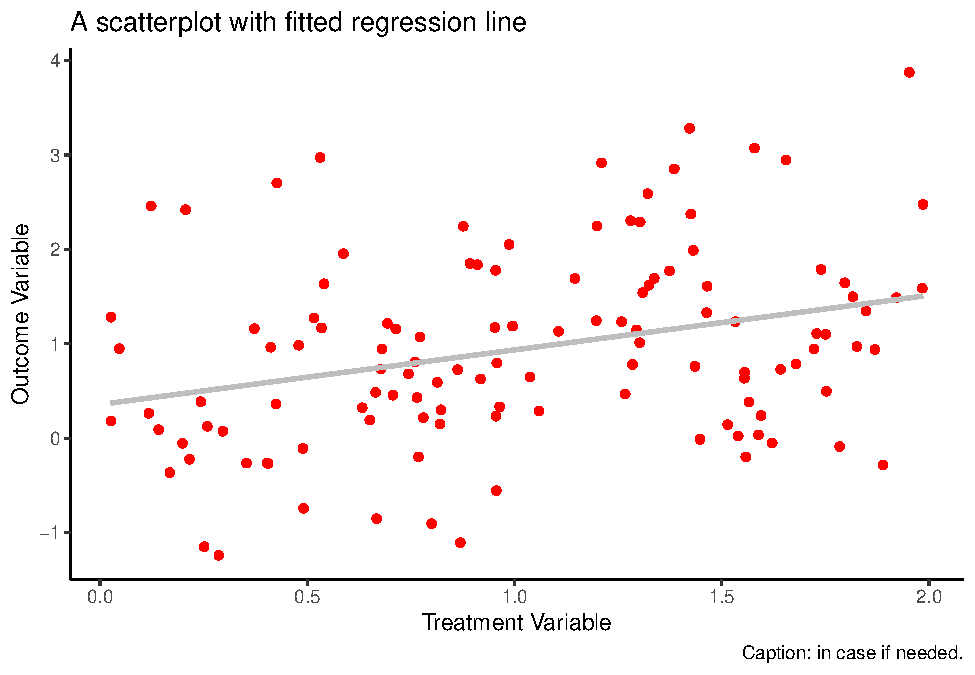
\includegraphics{forecasting_files/figure-latex/unnamed-chunk-29-1.pdf}

We can augment this plot in a number of different ways. Here we change the point color to red, add the fitted regression line to the plot, add labels to the figure, and apply a `classic' background theme:

\begin{Shaded}
\begin{Highlighting}[]
\FunctionTok{ggplot}\NormalTok{(dt,}\FunctionTok{aes}\NormalTok{(}\AttributeTok{x=}\NormalTok{x,}\AttributeTok{y=}\NormalTok{y))}\SpecialCharTok{+}
  \FunctionTok{geom\_point}\NormalTok{(}\AttributeTok{color=}\StringTok{"goldenrod"}\NormalTok{)}\SpecialCharTok{+}
  \FunctionTok{geom\_smooth}\NormalTok{(}\AttributeTok{method=}\StringTok{"lm"}\NormalTok{,}\AttributeTok{formula=}\NormalTok{y}\SpecialCharTok{\textasciitilde{}}\NormalTok{x,}\AttributeTok{se=}\NormalTok{F,}\AttributeTok{color=}\StringTok{"darkgray"}\NormalTok{)}\SpecialCharTok{+}
  \FunctionTok{labs}\NormalTok{(}\AttributeTok{title=}\StringTok{"A scatterplot with fitted regression line"}\NormalTok{, }
       \AttributeTok{x=}\StringTok{"Treatment Variable"}\NormalTok{, }
       \AttributeTok{y=}\StringTok{"Outcome Variable"}\NormalTok{, }
       \AttributeTok{caption=}\StringTok{"Caption: in case if needed."}\NormalTok{)}\SpecialCharTok{+}
  \FunctionTok{theme\_classic}\NormalTok{()}
\end{Highlighting}
\end{Shaded}

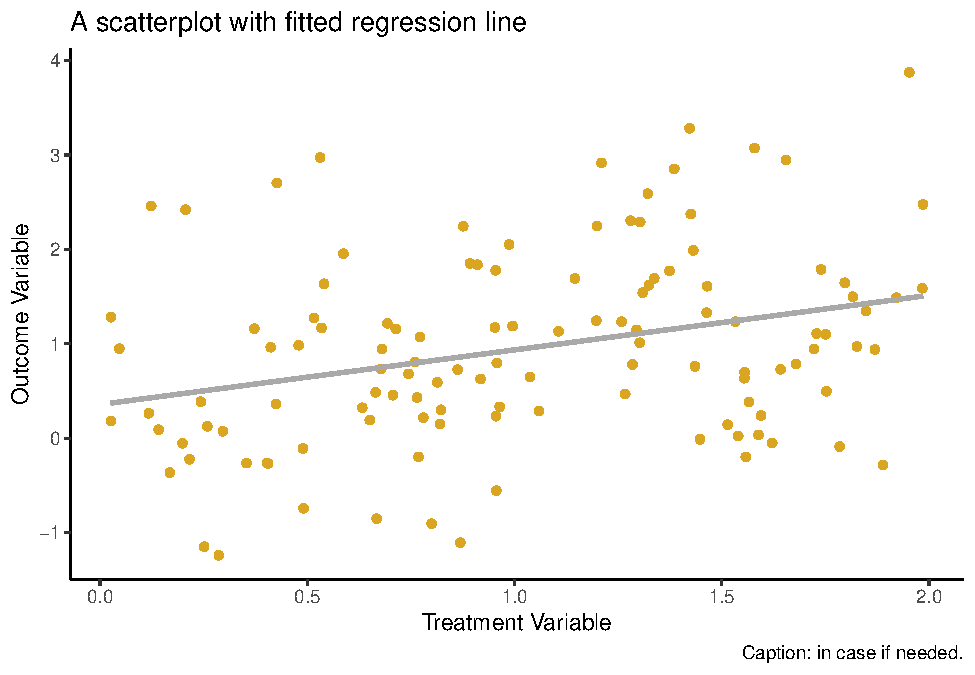
\includegraphics{forecasting_files/figure-latex/unnamed-chunk-30-1.pdf}

As another example, let's generate a histogram (of the dependent variable):

\begin{Shaded}
\begin{Highlighting}[]
\FunctionTok{ggplot}\NormalTok{(dt,}\FunctionTok{aes}\NormalTok{(}\AttributeTok{x=}\NormalTok{y))}\SpecialCharTok{+}
  \FunctionTok{geom\_histogram}\NormalTok{(}\AttributeTok{color=}\StringTok{"white"}\NormalTok{,}\AttributeTok{fill=}\StringTok{"goldenrod"}\NormalTok{,}\AttributeTok{binwidth=}\NormalTok{.}\DecValTok{5}\NormalTok{)}\SpecialCharTok{+}
  \FunctionTok{labs}\NormalTok{(}\AttributeTok{title=}\StringTok{"A basic histogram"}\NormalTok{)}\SpecialCharTok{+}
  \FunctionTok{theme\_classic}\NormalTok{()}
\end{Highlighting}
\end{Shaded}

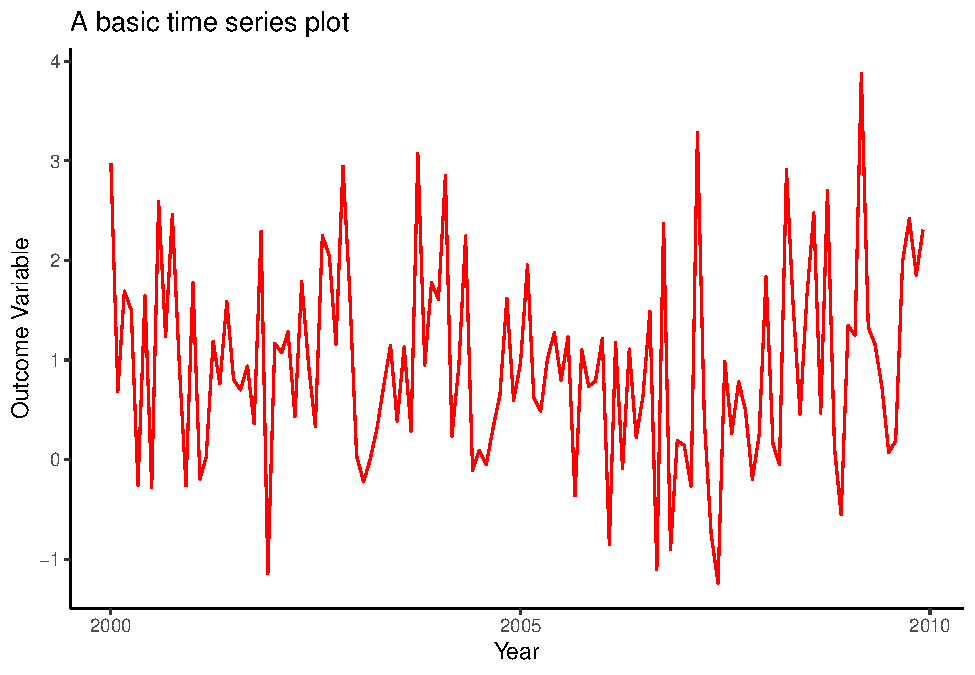
\includegraphics{forecasting_files/figure-latex/unnamed-chunk-31-1.pdf}

We typically apply a line plot to illustrate a time series (that are ordered by date). In what follows, we add a date column to our data frame and then plot the dependent variable in the chronological order:

\begin{Shaded}
\begin{Highlighting}[]
\NormalTok{dt}\SpecialCharTok{$}\NormalTok{date }\OtherTok{\textless{}{-}} \FunctionTok{seq}\NormalTok{(}\AttributeTok{from=}\FunctionTok{as.Date}\NormalTok{(}\StringTok{"2000{-}01{-}01"}\NormalTok{),}\AttributeTok{by=}\StringTok{"month"}\NormalTok{,}\AttributeTok{along.with=}\NormalTok{y)}

\FunctionTok{ggplot}\NormalTok{(dt,}\FunctionTok{aes}\NormalTok{(}\AttributeTok{x=}\NormalTok{date,}\AttributeTok{y=}\NormalTok{y))}\SpecialCharTok{+}
  \FunctionTok{geom\_line}\NormalTok{(}\AttributeTok{color=}\StringTok{"goldenrod"}\NormalTok{)}\SpecialCharTok{+}
  \FunctionTok{labs}\NormalTok{(}\AttributeTok{title=}\StringTok{"A basic time series plot"}\NormalTok{,  }
       \AttributeTok{x=}\StringTok{"Year"}\NormalTok{, }
       \AttributeTok{y=}\StringTok{"Outcome Variable"}\NormalTok{)}\SpecialCharTok{+}
  \FunctionTok{theme\_classic}\NormalTok{()}
\end{Highlighting}
\end{Shaded}

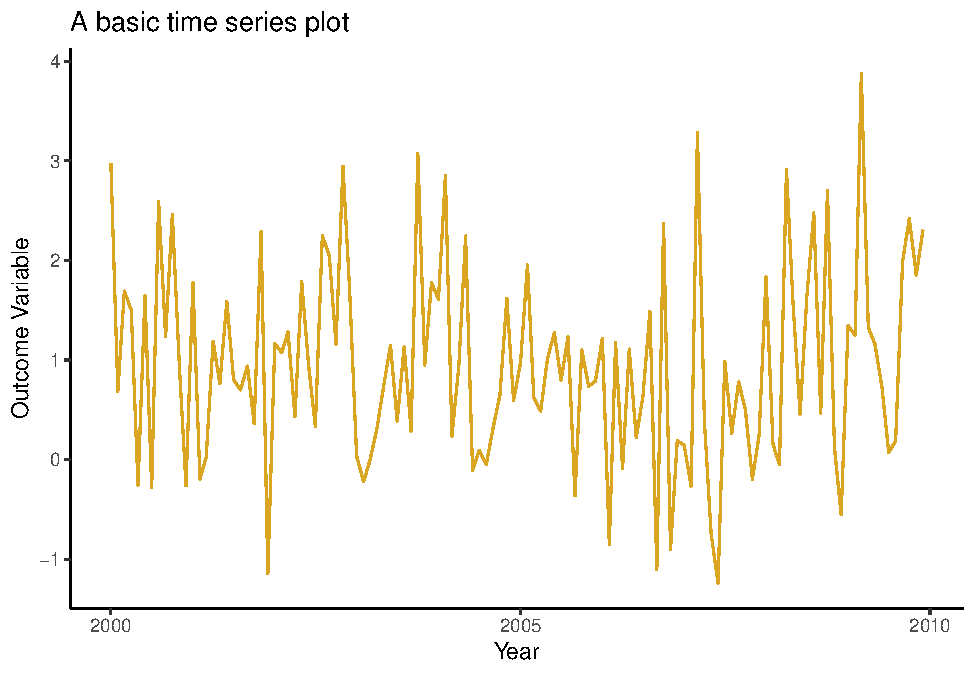
\includegraphics{forecasting_files/figure-latex/unnamed-chunk-32-1.pdf}

\hypertarget{regression-analysis}{%
\section*{Regression Analysis}\label{regression-analysis}}
\addcontentsline{toc}{section}{Regression Analysis}

To illustrate the OLS regression in R, we apply the previously generated \(x\) and \(y\) as independent and dependent variables. To begin, we obtain the least squares estimator ``by hand'' as follows:

\begin{Shaded}
\begin{Highlighting}[]
\NormalTok{X }\OtherTok{\textless{}{-}} \FunctionTok{cbind}\NormalTok{(}\DecValTok{1}\NormalTok{,x)}
\NormalTok{b }\OtherTok{\textless{}{-}} \FunctionTok{solve}\NormalTok{(}\FunctionTok{t}\NormalTok{(X)}\SpecialCharTok{\%*\%}\NormalTok{X)}\SpecialCharTok{\%*\%}\FunctionTok{t}\NormalTok{(X)}\SpecialCharTok{\%*\%}\NormalTok{y}
\NormalTok{b}
\end{Highlighting}
\end{Shaded}

\begin{verbatim}
##        [,1]
##   0.3577680
## x 0.5781188
\end{verbatim}

This can be easily done using the lm() function:

\begin{Shaded}
\begin{Highlighting}[]
\NormalTok{ols }\OtherTok{\textless{}{-}} \FunctionTok{lm}\NormalTok{(y}\SpecialCharTok{\textasciitilde{}}\NormalTok{x)}
\NormalTok{ols}
\end{Highlighting}
\end{Shaded}

\begin{verbatim}
## 
## Call:
## lm(formula = y ~ x)
## 
## Coefficients:
## (Intercept)            x  
##      0.3578       0.5781
\end{verbatim}

We can apply the summary() function to see the complete set of regression results:

\begin{Shaded}
\begin{Highlighting}[]
\FunctionTok{summary}\NormalTok{(ols)}
\end{Highlighting}
\end{Shaded}

\begin{verbatim}
## 
## Call:
## lm(formula = y ~ x)
## 
## Residuals:
##     Min      1Q  Median      3Q     Max 
## -1.9662 -0.5983 -0.1127  0.5639  2.3882 
## 
## Coefficients:
##             Estimate Std. Error t value Pr(>|t|)    
## (Intercept)   0.3578     0.1904   1.879 0.062717 .  
## x             0.5781     0.1641   3.522 0.000609 ***
## ---
## Signif. codes:  0 '***' 0.001 '**' 0.01 '*' 0.05 '.' 0.1 ' ' 1
## 
## Residual standard error: 0.9716 on 118 degrees of freedom
## Multiple R-squared:  0.09514,    Adjusted R-squared:  0.08748 
## F-statistic: 12.41 on 1 and 118 DF,  p-value: 0.0006091
\end{verbatim}

\hypertarget{tutorial-2-some-r-functions}{%
\chapter*{Tutorial 2: Some R Functions}\label{tutorial-2-some-r-functions}}
\addcontentsline{toc}{chapter}{Tutorial 2: Some R Functions}

In this tutorial, we will introduce several simple R functions, and will perform a basic forecasting exercise.

Let's generate a sequence of 200 iid random variables with mean zero and variance 4, call it e.

\begin{Shaded}
\begin{Highlighting}[]
\FunctionTok{set.seed}\NormalTok{(}\DecValTok{1}\NormalTok{)}
\NormalTok{e }\OtherTok{\textless{}{-}} \FunctionTok{rnorm}\NormalTok{(}\DecValTok{200}\NormalTok{,}\DecValTok{0}\NormalTok{,}\DecValTok{2}\NormalTok{)}
\end{Highlighting}
\end{Shaded}

Notice that prior to sampling we set seed to some value (to one in this instance). We do so to ensure that we can exactly replicate the sample in the future.

Nett, generate a sequence of 200 binary variables, call it x.

\begin{Shaded}
\begin{Highlighting}[]
\FunctionTok{set.seed}\NormalTok{(}\DecValTok{2}\NormalTok{)}
\NormalTok{x }\OtherTok{\textless{}{-}} \FunctionTok{sample}\NormalTok{(}\FunctionTok{c}\NormalTok{(}\DecValTok{0}\NormalTok{,}\DecValTok{1}\NormalTok{),}\DecValTok{200}\NormalTok{,}\AttributeTok{replace=}\NormalTok{T)}
\end{Highlighting}
\end{Shaded}

Construct a dependent variable, y, using the following formula: \(y=2+0.5x+e\).

\begin{Shaded}
\begin{Highlighting}[]
\NormalTok{y }\OtherTok{\textless{}{-}} \DecValTok{2}\FloatTok{+0.5}\SpecialCharTok{*}\NormalTok{x}\SpecialCharTok{+}\NormalTok{e}
\end{Highlighting}
\end{Shaded}

Regress y on x, using the \texttt{lm()} function, to obtain estimates of the intercept and slope parameters.

\begin{Shaded}
\begin{Highlighting}[]
\NormalTok{ols }\OtherTok{\textless{}{-}} \FunctionTok{lm}\NormalTok{(y}\SpecialCharTok{\textasciitilde{}}\NormalTok{x)}
\NormalTok{ols}
\end{Highlighting}
\end{Shaded}

\begin{verbatim}
## 
## Call:
## lm(formula = y ~ x)
## 
## Coefficients:
## (Intercept)            x  
##      2.1244       0.3854
\end{verbatim}

Generate some ``future'' realizations (100 observations) of y.

\begin{Shaded}
\begin{Highlighting}[]
\FunctionTok{set.seed}\NormalTok{(}\DecValTok{3}\NormalTok{)}
\NormalTok{e }\OtherTok{\textless{}{-}} \FunctionTok{rnorm}\NormalTok{(}\DecValTok{100}\NormalTok{,}\DecValTok{0}\NormalTok{,}\DecValTok{2}\NormalTok{)}

\FunctionTok{set.seed}\NormalTok{(}\DecValTok{4}\NormalTok{)}
\NormalTok{x }\OtherTok{\textless{}{-}} \FunctionTok{sample}\NormalTok{(}\FunctionTok{c}\NormalTok{(}\DecValTok{0}\NormalTok{,}\DecValTok{1}\NormalTok{),}\DecValTok{100}\NormalTok{,}\AttributeTok{replace=}\NormalTok{T)}

\NormalTok{y }\OtherTok{\textless{}{-}} \DecValTok{2}\FloatTok{+0.5}\SpecialCharTok{*}\NormalTok{x}\SpecialCharTok{+}\NormalTok{e}
\end{Highlighting}
\end{Shaded}

Note that these represent actual realizations of the variable; these not forecasts.

Suppose we think that in the considered forecast period, x only takes on 1 (below we will refer to this as the Model 1). Based on this, and using parameter estimates from above, let's generate forecasts for this period.

\begin{Shaded}
\begin{Highlighting}[]
\NormalTok{y\_f1 }\OtherTok{\textless{}{-}}\NormalTok{ ols}\SpecialCharTok{$}\NormalTok{coefficients[}\DecValTok{1}\NormalTok{]}\SpecialCharTok{+}\NormalTok{ols}\SpecialCharTok{$}\NormalTok{coefficients[}\DecValTok{2}\NormalTok{]}\SpecialCharTok{*}\FunctionTok{rep}\NormalTok{(}\DecValTok{1}\NormalTok{,}\DecValTok{100}\NormalTok{)}
\end{Highlighting}
\end{Shaded}

At this point, we have actual realisations of y and its forecasts. Thus, we can obtain forecast errors, mean absolute forecast errors, and root mean square forecast errors.

\begin{Shaded}
\begin{Highlighting}[]
\NormalTok{e\_f1 }\OtherTok{\textless{}{-}}\NormalTok{ y}\SpecialCharTok{{-}}\NormalTok{y\_f1}

\NormalTok{mafe1 }\OtherTok{\textless{}{-}} \FunctionTok{mean}\NormalTok{(}\FunctionTok{abs}\NormalTok{(e\_f1))}
\NormalTok{rmsfe1 }\OtherTok{\textless{}{-}} \FunctionTok{sqrt}\NormalTok{(}\FunctionTok{mean}\NormalTok{(e\_f1}\SpecialCharTok{\^{}}\DecValTok{2}\NormalTok{))}

\NormalTok{mafe1}
\end{Highlighting}
\end{Shaded}

\begin{verbatim}
## [1] 1.43523
\end{verbatim}

\begin{Shaded}
\begin{Highlighting}[]
\NormalTok{rmsfe1}
\end{Highlighting}
\end{Shaded}

\begin{verbatim}
## [1] 1.739508
\end{verbatim}

Suppose, instead, we think that in the considered forecast period x only takes on 0 (below we will refer to this as the Model 2). Based on this, and using parameter estimates from above, let's generate forecasts for this period.

\begin{Shaded}
\begin{Highlighting}[]
\NormalTok{y\_f0 }\OtherTok{\textless{}{-}}\NormalTok{ ols}\SpecialCharTok{$}\NormalTok{coefficients[}\DecValTok{1}\NormalTok{]}\SpecialCharTok{+}\NormalTok{ols}\SpecialCharTok{$}\NormalTok{coefficients[}\DecValTok{2}\NormalTok{]}\SpecialCharTok{*}\FunctionTok{rep}\NormalTok{(}\DecValTok{0}\NormalTok{,}\DecValTok{100}\NormalTok{)}
\end{Highlighting}
\end{Shaded}

Using these forecasts, obtain forecast errors, mean absolute forecast errors, and root mean square forecast errors.

\begin{Shaded}
\begin{Highlighting}[]
\NormalTok{e\_f0 }\OtherTok{\textless{}{-}}\NormalTok{ y}\SpecialCharTok{{-}}\NormalTok{y\_f0}

\NormalTok{mafe0 }\OtherTok{\textless{}{-}} \FunctionTok{mean}\NormalTok{(}\FunctionTok{abs}\NormalTok{(e\_f0))}
\NormalTok{rmsfe0 }\OtherTok{\textless{}{-}} \FunctionTok{sqrt}\NormalTok{(}\FunctionTok{mean}\NormalTok{(e\_f0}\SpecialCharTok{\^{}}\DecValTok{2}\NormalTok{))}

\NormalTok{mafe0}
\end{Highlighting}
\end{Shaded}

\begin{verbatim}
## [1] 1.455768
\end{verbatim}

\begin{Shaded}
\begin{Highlighting}[]
\NormalTok{rmsfe0}
\end{Highlighting}
\end{Shaded}

\begin{verbatim}
## [1] 1.736182
\end{verbatim}

By comparing the two sets of forecasts, we can observe a somewhat rare and yet not an unlikely scenario: MAFE points to the Model 1 as more accurate of the two models, while RMSFE suggests the Model 2 as the more accurate one. More often than not, however, these two accuracy measures tend to agree.

\hypertarget{tutorial-3-forecasting-methods-and-routines}{%
\chapter*{Tutorial 3: Forecasting Methods and Routines}\label{tutorial-3-forecasting-methods-and-routines}}
\addcontentsline{toc}{chapter}{Tutorial 3: Forecasting Methods and Routines}

In this tutorial, we will introduce `for loop,' and use it to generate time series as well as to obtain one-step-ahead forecasts using a rolling window procedure; we will also perform forecast error diagnostics.

Let's generate a random walk process, such that \(y_{t} = y_{t-1}+e_{t}\), where \(e_{t} ~ N(0,1)\), and where \(y_{0}=0\), for \(t=1,\ldots,120\).

\begin{Shaded}
\begin{Highlighting}[]
\NormalTok{n }\OtherTok{\textless{}{-}} \DecValTok{120}

\FunctionTok{set.seed}\NormalTok{(}\DecValTok{1}\NormalTok{)}
\NormalTok{e }\OtherTok{\textless{}{-}} \FunctionTok{rnorm}\NormalTok{(n)}

\NormalTok{y }\OtherTok{\textless{}{-}} \FunctionTok{rep}\NormalTok{(}\ConstantTok{NA}\NormalTok{,n)}

\NormalTok{y[}\DecValTok{1}\NormalTok{] }\OtherTok{\textless{}{-}}\NormalTok{ e[}\DecValTok{1}\NormalTok{]}

\ControlFlowTok{for}\NormalTok{(i }\ControlFlowTok{in} \DecValTok{2}\SpecialCharTok{:}\NormalTok{n)\{}
\NormalTok{  y[i] }\OtherTok{\textless{}{-}}\NormalTok{ y[i}\DecValTok{{-}1}\NormalTok{] }\SpecialCharTok{+}\NormalTok{ e[i]}
\NormalTok{\}}
\end{Highlighting}
\end{Shaded}

Store \(y\) and \(e\) in a \textbf{data.table}, call it `dt.' Add some arbitrary dates to the data (e.g., suppose we deal with the monthly series beginning from January 2011).

\begin{Shaded}
\begin{Highlighting}[]
\NormalTok{dt }\OtherTok{\textless{}{-}} \FunctionTok{data.table}\NormalTok{(y,e)}

\NormalTok{dt}\SpecialCharTok{$}\NormalTok{date }\OtherTok{\textless{}{-}} \FunctionTok{seq}\NormalTok{(}\FunctionTok{as.Date}\NormalTok{(}\StringTok{"2011{-}01{-}01"}\NormalTok{),}\FunctionTok{as.Date}\NormalTok{(}\StringTok{"2020{-}12{-}01"}\NormalTok{),}\AttributeTok{by=}\StringTok{"month"}\NormalTok{)}
\end{Highlighting}
\end{Shaded}

Plot the realized time series using \textbf{ggplot} function.

\begin{Shaded}
\begin{Highlighting}[]
\FunctionTok{ggplot}\NormalTok{(dt,}\FunctionTok{aes}\NormalTok{(}\AttributeTok{x=}\NormalTok{date,}\AttributeTok{y=}\NormalTok{y))}\SpecialCharTok{+}
  \FunctionTok{geom\_line}\NormalTok{(}\AttributeTok{size=}\DecValTok{1}\NormalTok{)}\SpecialCharTok{+}
  \FunctionTok{labs}\NormalTok{(}\AttributeTok{x=}\StringTok{"Year"}\NormalTok{,}\AttributeTok{y=}\StringTok{"Random Walk"}\NormalTok{)}\SpecialCharTok{+}
  \FunctionTok{theme\_classic}\NormalTok{()}
\end{Highlighting}
\end{Shaded}

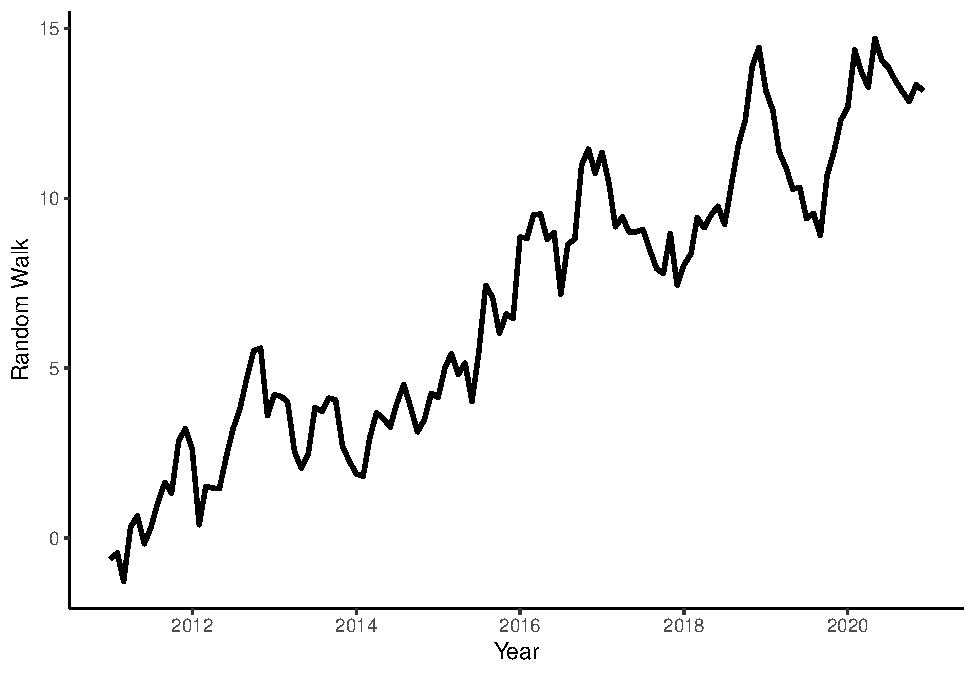
\includegraphics{forecasting_files/figure-latex/unnamed-chunk-49-1.pdf}

Generate a sequence of one-step-ahead forecasts from naive and average methods, using the rolling window scheme, where the first rolling window ranges from period 1 to period 80.

\begin{Shaded}
\begin{Highlighting}[]
\NormalTok{dt}\SpecialCharTok{$}\NormalTok{average }\OtherTok{\textless{}{-}} \ConstantTok{NA}
\NormalTok{dt}\SpecialCharTok{$}\NormalTok{naive }\OtherTok{\textless{}{-}} \ConstantTok{NA}

\NormalTok{R }\OtherTok{\textless{}{-}} \DecValTok{80}
\NormalTok{P }\OtherTok{\textless{}{-}}\NormalTok{ n}\SpecialCharTok{{-}}\NormalTok{R}
\ControlFlowTok{for}\NormalTok{(i }\ControlFlowTok{in} \DecValTok{1}\SpecialCharTok{:}\NormalTok{P)\{}
\NormalTok{  w }\OtherTok{\textless{}{-}}\NormalTok{ y[i}\SpecialCharTok{:}\NormalTok{(R}\DecValTok{{-}1}\SpecialCharTok{+}\NormalTok{i)]}
\NormalTok{  dt}\SpecialCharTok{$}\NormalTok{average[R}\SpecialCharTok{+}\NormalTok{i] }\OtherTok{\textless{}{-}} \FunctionTok{mean}\NormalTok{(w)}
\NormalTok{  dt}\SpecialCharTok{$}\NormalTok{naive[R}\SpecialCharTok{+}\NormalTok{i] }\OtherTok{\textless{}{-}}\NormalTok{ w[}\FunctionTok{length}\NormalTok{(w)]}
\NormalTok{\}}
\end{Highlighting}
\end{Shaded}

Calculate the RMSFE measures for each of the two forecasting methods.

\begin{Shaded}
\begin{Highlighting}[]
\NormalTok{dt[,}\StringTok{\textasciigrave{}}\AttributeTok{:=}\StringTok{\textasciigrave{}}\NormalTok{(}\AttributeTok{e\_average=}\NormalTok{y}\SpecialCharTok{{-}}\NormalTok{average,}\AttributeTok{e\_naive=}\NormalTok{y}\SpecialCharTok{{-}}\NormalTok{naive)]}

\NormalTok{rmsfe\_average }\OtherTok{\textless{}{-}} \FunctionTok{sqrt}\NormalTok{(}\FunctionTok{mean}\NormalTok{(dt}\SpecialCharTok{$}\NormalTok{e\_average}\SpecialCharTok{\^{}}\DecValTok{2}\NormalTok{,}\AttributeTok{na.rm=}\NormalTok{T))}
\NormalTok{rmsfe\_naive }\OtherTok{\textless{}{-}} \FunctionTok{sqrt}\NormalTok{(}\FunctionTok{mean}\NormalTok{(dt}\SpecialCharTok{$}\NormalTok{e\_naive}\SpecialCharTok{\^{}}\DecValTok{2}\NormalTok{,}\AttributeTok{na.rm=}\NormalTok{T))}

\NormalTok{rmsfe\_average}
\end{Highlighting}
\end{Shaded}

\begin{verbatim}
## [1] 4.672947
\end{verbatim}

\begin{Shaded}
\begin{Highlighting}[]
\NormalTok{rmsfe\_naive}
\end{Highlighting}
\end{Shaded}

\begin{verbatim}
## [1] 0.850081
\end{verbatim}

Perform the forecast error diagnostics for the two considered methods.

Zero mean of the forecast errors: \(E(e_{t+1|t})=0\).
We perform this test by regressing the forecast error on the constant, and checking whether the coefficient is statistically significantly different from zero.

\begin{Shaded}
\begin{Highlighting}[]
\FunctionTok{summary}\NormalTok{(}\FunctionTok{lm}\NormalTok{(e\_average}\SpecialCharTok{\textasciitilde{}}\DecValTok{1}\NormalTok{,}\AttributeTok{data=}\NormalTok{dt))}\SpecialCharTok{$}\NormalTok{coefficients}
\end{Highlighting}
\end{Shaded}

\begin{verbatim}
##             Estimate Std. Error  t value     Pr(>|t|)
## (Intercept) 4.434858  0.2358002 18.80769 3.682273e-21
\end{verbatim}

\begin{Shaded}
\begin{Highlighting}[]
\FunctionTok{summary}\NormalTok{(}\FunctionTok{lm}\NormalTok{(e\_naive}\SpecialCharTok{\textasciitilde{}}\DecValTok{1}\NormalTok{,}\AttributeTok{data=}\NormalTok{dt))}\SpecialCharTok{$}\NormalTok{coefficients}
\end{Highlighting}
\end{Shaded}

\begin{verbatim}
##              Estimate Std. Error t value Pr(>|t|)
## (Intercept) 0.1168396    0.13483 0.86657 0.391478
\end{verbatim}

No correlation of the forecast errors with the forecasts: \(Cov(e_{t+1|t},y_{t+1|t})=0\). We perform this test by regressing the forecast error on the forecast, and checking whether the slope coefficient is statistically significantly different from zero.

\begin{Shaded}
\begin{Highlighting}[]
\FunctionTok{summary}\NormalTok{(}\FunctionTok{lm}\NormalTok{(e\_average}\SpecialCharTok{\textasciitilde{}}\NormalTok{average,}\AttributeTok{data=}\NormalTok{dt))}\SpecialCharTok{$}\NormalTok{coefficients}
\end{Highlighting}
\end{Shaded}

\begin{verbatim}
##              Estimate Std. Error  t value   Pr(>|t|)
## (Intercept) 2.4180785  1.2929708 1.870172 0.06917788
## average     0.2942557  0.1856048 1.585389 0.12116580
\end{verbatim}

\begin{Shaded}
\begin{Highlighting}[]
\FunctionTok{summary}\NormalTok{(}\FunctionTok{lm}\NormalTok{(e\_naive}\SpecialCharTok{\textasciitilde{}}\NormalTok{naive,}\AttributeTok{data=}\NormalTok{dt))}\SpecialCharTok{$}\NormalTok{coefficients}
\end{Highlighting}
\end{Shaded}

\begin{verbatim}
##                Estimate Std. Error   t value  Pr(>|t|)
## (Intercept)  1.06489905 0.69740557  1.526944 0.1350565
## naive       -0.08486143 0.06127484 -1.384931 0.1741512
\end{verbatim}

No serial correlation in one-step-ahead forecast errors: \(Cov(e_{t+1|t},y_{t|t-1})=0\). We perform this test by regressing the forecast error on its lag, and checking whether the slope coefficient is statistically significantly different from zero.
(Note: first we need to generate lagged forecast errors)

\begin{Shaded}
\begin{Highlighting}[]
\NormalTok{dt[,}\StringTok{\textasciigrave{}}\AttributeTok{:=}\StringTok{\textasciigrave{}}\NormalTok{(}\AttributeTok{e\_average.l1=}\FunctionTok{shift}\NormalTok{(e\_average),}\AttributeTok{e\_naive.l1=}\FunctionTok{shift}\NormalTok{(e\_naive))]}

\FunctionTok{summary}\NormalTok{(}\FunctionTok{lm}\NormalTok{(e\_average}\SpecialCharTok{\textasciitilde{}}\NormalTok{e\_average.l1,}\AttributeTok{data=}\NormalTok{dt))}\SpecialCharTok{$}\NormalTok{coefficients}
\end{Highlighting}
\end{Shaded}

\begin{verbatim}
##               Estimate Std. Error  t value     Pr(>|t|)
## (Intercept)  0.7898068 0.42027705 1.879253 6.810403e-02
## e_average.l1 0.8275396 0.08966026 9.229726 3.892504e-11
\end{verbatim}

\begin{Shaded}
\begin{Highlighting}[]
\FunctionTok{summary}\NormalTok{(}\FunctionTok{lm}\NormalTok{(e\_naive}\SpecialCharTok{\textasciitilde{}}\NormalTok{e\_naive.l1,}\AttributeTok{data=}\NormalTok{dt))}\SpecialCharTok{$}\NormalTok{coefficients}
\end{Highlighting}
\end{Shaded}

\begin{verbatim}
##               Estimate Std. Error   t value  Pr(>|t|)
## (Intercept) 0.12971406  0.1403668 0.9241081 0.3614178
## e_naive.l1  0.03780853  0.1631333 0.2317647 0.8179979
\end{verbatim}

\hypertarget{tutorial-4-deterministic-trends}{%
\chapter*{Tutorial 4: Deterministic Trends}\label{tutorial-4-deterministic-trends}}
\addcontentsline{toc}{chapter}{Tutorial 4: Deterministic Trends}

In this tutorial, we will generate trending series, we will apply an information criterion to select the most suitable trend model, and we will obtain and compare one-step-ahead forecasts using a rolling window procedure.

Let's generate a time series that follows a quadratic trend: \(y_{t} = 10+0.01t+0.002t^2+e_{t}\), where \(e_{t} \sim N(0,16)\), for \(t=1,\ldots,180\).

\begin{Shaded}
\begin{Highlighting}[]
\NormalTok{n }\OtherTok{\textless{}{-}} \DecValTok{180}

\FunctionTok{set.seed}\NormalTok{(}\DecValTok{7}\NormalTok{)}
\NormalTok{e }\OtherTok{\textless{}{-}} \FunctionTok{rnorm}\NormalTok{(n,}\DecValTok{0}\NormalTok{,}\DecValTok{4}\NormalTok{)}

\NormalTok{trend }\OtherTok{\textless{}{-}} \FunctionTok{c}\NormalTok{(}\DecValTok{1}\SpecialCharTok{:}\NormalTok{n)}

\NormalTok{y }\OtherTok{\textless{}{-}} \DecValTok{10}\FloatTok{+0.01}\SpecialCharTok{*}\NormalTok{trend}\FloatTok{+0.002}\SpecialCharTok{*}\NormalTok{trend}\SpecialCharTok{\^{}}\DecValTok{2}\SpecialCharTok{+}\NormalTok{e}
\end{Highlighting}
\end{Shaded}

Store \(y\) and \(trend\) in a \textbf{data.table}, call it `dt.' Add some arbitrary dates to the data (e.g., suppose we deal with the monthly series beginning from January 2006).

\begin{Shaded}
\begin{Highlighting}[]
\NormalTok{dt }\OtherTok{\textless{}{-}} \FunctionTok{data.table}\NormalTok{(y,trend)}

\NormalTok{dt}\SpecialCharTok{$}\NormalTok{date }\OtherTok{\textless{}{-}} \FunctionTok{seq}\NormalTok{(}\FunctionTok{as.Date}\NormalTok{(}\StringTok{"2006{-}01{-}01"}\NormalTok{),}\AttributeTok{by=}\StringTok{"month"}\NormalTok{,}\AttributeTok{along.with=}\NormalTok{y)}
\end{Highlighting}
\end{Shaded}

Plot the realized time series using \textbf{ggplot} function.

\begin{Shaded}
\begin{Highlighting}[]
\FunctionTok{ggplot}\NormalTok{(dt,}\FunctionTok{aes}\NormalTok{(}\AttributeTok{x=}\NormalTok{date,}\AttributeTok{y=}\NormalTok{y))}\SpecialCharTok{+}
  \FunctionTok{geom\_line}\NormalTok{(}\AttributeTok{size=}\DecValTok{1}\NormalTok{)}\SpecialCharTok{+}
  \FunctionTok{labs}\NormalTok{(}\AttributeTok{x=}\StringTok{"Year"}\NormalTok{,}\AttributeTok{y=}\StringTok{"Trending Series"}\NormalTok{)}\SpecialCharTok{+}
  \FunctionTok{theme\_classic}\NormalTok{()}
\end{Highlighting}
\end{Shaded}

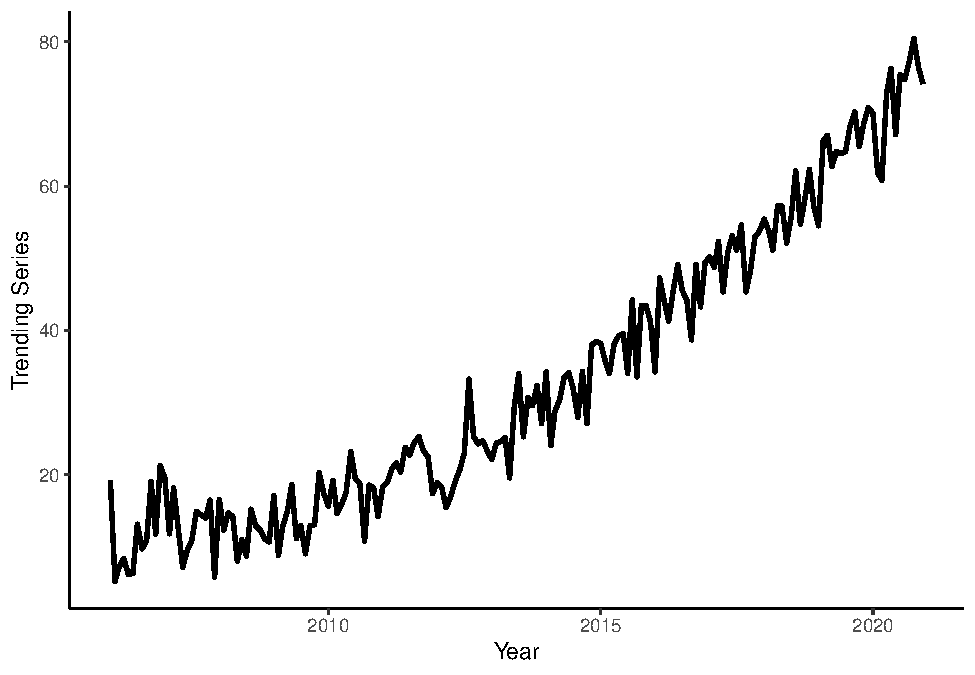
\includegraphics{forecasting_files/figure-latex/unnamed-chunk-58-1.pdf}

Calculate Akaike Information Criteria for linear, quadratic, cubic, and exponential trend models, using all observations in the series.

\begin{Shaded}
\begin{Highlighting}[]
\NormalTok{AIC\_vec }\OtherTok{\textless{}{-}} \FunctionTok{matrix}\NormalTok{(}\AttributeTok{ncol=}\DecValTok{4}\NormalTok{,}\AttributeTok{nrow=}\DecValTok{1}\NormalTok{)}
\ControlFlowTok{for}\NormalTok{(i }\ControlFlowTok{in} \DecValTok{1}\SpecialCharTok{:}\DecValTok{4}\NormalTok{)\{}
  \ControlFlowTok{if}\NormalTok{(i }\SpecialCharTok{\textless{}} \DecValTok{4}\NormalTok{)\{}
\NormalTok{    reg }\OtherTok{\textless{}{-}} \FunctionTok{lm}\NormalTok{(y}\SpecialCharTok{\textasciitilde{}}\FunctionTok{poly}\NormalTok{(trend,}\AttributeTok{degree=}\NormalTok{i,}\AttributeTok{raw=}\NormalTok{T),}\AttributeTok{data=}\NormalTok{dt)}
\NormalTok{    AIC\_vec[i] }\OtherTok{\textless{}{-}} \FunctionTok{log}\NormalTok{(}\FunctionTok{crossprod}\NormalTok{(reg}\SpecialCharTok{$}\NormalTok{residuals))}\SpecialCharTok{+}\DecValTok{2}\SpecialCharTok{*}\FunctionTok{length}\NormalTok{(reg}\SpecialCharTok{$}\NormalTok{coefficients)}\SpecialCharTok{/}\NormalTok{n}
\NormalTok{  \}}\ControlFlowTok{else}\NormalTok{\{}
\NormalTok{    reg }\OtherTok{\textless{}{-}} \FunctionTok{lm}\NormalTok{(}\FunctionTok{log}\NormalTok{(y)}\SpecialCharTok{\textasciitilde{}}\NormalTok{trend,}\AttributeTok{data=}\NormalTok{dt)}
\NormalTok{    yhat }\OtherTok{\textless{}{-}}\NormalTok{ reg}\SpecialCharTok{$}\NormalTok{fitted.values}
\NormalTok{    sig }\OtherTok{\textless{}{-}} \FunctionTok{sd}\NormalTok{(reg}\SpecialCharTok{$}\NormalTok{residuals)}
\NormalTok{    ystar }\OtherTok{\textless{}{-}} \FunctionTok{exp}\NormalTok{(yhat}\SpecialCharTok{+}\NormalTok{sig}\SpecialCharTok{\^{}}\DecValTok{2}\SpecialCharTok{/}\DecValTok{2}\NormalTok{)}
\NormalTok{    res }\OtherTok{\textless{}{-}}\NormalTok{ dt}\SpecialCharTok{$}\NormalTok{y}\SpecialCharTok{{-}}\NormalTok{ystar}
\NormalTok{    AIC\_vec[i] }\OtherTok{\textless{}{-}} \FunctionTok{log}\NormalTok{(}\FunctionTok{crossprod}\NormalTok{(res))}\SpecialCharTok{+}\DecValTok{2}\SpecialCharTok{*}\FunctionTok{length}\NormalTok{(reg}\SpecialCharTok{$}\NormalTok{coefficients)}\SpecialCharTok{/}\NormalTok{n}
\NormalTok{  \}}
\NormalTok{\}}

\NormalTok{AIC\_vec}
\end{Highlighting}
\end{Shaded}

\begin{verbatim}
##          [,1]     [,2]     [,3]     [,4]
## [1,] 8.879646 7.841645 7.849521 7.975999
\end{verbatim}

Generate a sequence of one-step-ahead forecasts from linear, quadratic, cubic, and exponential trend models, using the rolling window scheme, where the first rolling window ranges from period 1 to period 120.

\begin{Shaded}
\begin{Highlighting}[]
\NormalTok{dt}\SpecialCharTok{$}\NormalTok{t1 }\OtherTok{\textless{}{-}} \ConstantTok{NA}
\NormalTok{dt}\SpecialCharTok{$}\NormalTok{t2 }\OtherTok{\textless{}{-}} \ConstantTok{NA}
\NormalTok{dt}\SpecialCharTok{$}\NormalTok{t3 }\OtherTok{\textless{}{-}} \ConstantTok{NA}
\NormalTok{dt}\SpecialCharTok{$}\NormalTok{te }\OtherTok{\textless{}{-}} \ConstantTok{NA}

\NormalTok{R }\OtherTok{\textless{}{-}} \DecValTok{120}
\NormalTok{P }\OtherTok{\textless{}{-}}\NormalTok{ n}\SpecialCharTok{{-}}\NormalTok{R}
\ControlFlowTok{for}\NormalTok{(i }\ControlFlowTok{in} \DecValTok{1}\SpecialCharTok{:}\NormalTok{P)\{}
\NormalTok{  reg1 }\OtherTok{\textless{}{-}} \FunctionTok{lm}\NormalTok{(y}\SpecialCharTok{\textasciitilde{}}\NormalTok{trend,}\AttributeTok{data=}\NormalTok{dt[i}\SpecialCharTok{:}\NormalTok{(R}\DecValTok{{-}1}\SpecialCharTok{+}\NormalTok{i)])}
\NormalTok{  dt}\SpecialCharTok{$}\NormalTok{t1[R}\SpecialCharTok{+}\NormalTok{i] }\OtherTok{\textless{}{-}}\NormalTok{ reg1}\SpecialCharTok{$}\NormalTok{coef[}\DecValTok{1}\NormalTok{]}\SpecialCharTok{+}\NormalTok{reg1}\SpecialCharTok{$}\NormalTok{coef[}\DecValTok{2}\NormalTok{]}\SpecialCharTok{*}\NormalTok{(R}\SpecialCharTok{+}\NormalTok{i)}
  
\NormalTok{  reg2 }\OtherTok{\textless{}{-}} \FunctionTok{lm}\NormalTok{(y}\SpecialCharTok{\textasciitilde{}}\FunctionTok{poly}\NormalTok{(trend,}\AttributeTok{degree=}\DecValTok{2}\NormalTok{,}\AttributeTok{raw=}\NormalTok{T),}\AttributeTok{data=}\NormalTok{dt[i}\SpecialCharTok{:}\NormalTok{(R}\DecValTok{{-}1}\SpecialCharTok{+}\NormalTok{i)])}
\NormalTok{  dt}\SpecialCharTok{$}\NormalTok{t2[R}\SpecialCharTok{+}\NormalTok{i] }\OtherTok{\textless{}{-}}\NormalTok{ reg2}\SpecialCharTok{$}\NormalTok{coef[}\DecValTok{1}\NormalTok{]}\SpecialCharTok{+}\NormalTok{reg2}\SpecialCharTok{$}\NormalTok{coef[}\DecValTok{2}\NormalTok{]}\SpecialCharTok{*}\NormalTok{(R}\SpecialCharTok{+}\NormalTok{i)}\SpecialCharTok{+}\NormalTok{reg2}\SpecialCharTok{$}\NormalTok{coef[}\DecValTok{3}\NormalTok{]}\SpecialCharTok{*}\NormalTok{((R}\SpecialCharTok{+}\NormalTok{i)}\SpecialCharTok{\^{}}\DecValTok{2}\NormalTok{)}
  
\NormalTok{  reg3 }\OtherTok{\textless{}{-}} \FunctionTok{lm}\NormalTok{(y}\SpecialCharTok{\textasciitilde{}}\FunctionTok{poly}\NormalTok{(trend,}\AttributeTok{degree=}\DecValTok{3}\NormalTok{,}\AttributeTok{raw=}\NormalTok{T),}\AttributeTok{data=}\NormalTok{dt[i}\SpecialCharTok{:}\NormalTok{(R}\DecValTok{{-}1}\SpecialCharTok{+}\NormalTok{i)])}
\NormalTok{  dt}\SpecialCharTok{$}\NormalTok{t3[R}\SpecialCharTok{+}\NormalTok{i] }\OtherTok{\textless{}{-}}\NormalTok{ reg3}\SpecialCharTok{$}\NormalTok{coef[}\DecValTok{1}\NormalTok{]}\SpecialCharTok{+}\NormalTok{reg3}\SpecialCharTok{$}\NormalTok{coef[}\DecValTok{2}\NormalTok{]}\SpecialCharTok{*}\NormalTok{(R}\SpecialCharTok{+}\NormalTok{i)}\SpecialCharTok{+}\NormalTok{reg3}\SpecialCharTok{$}\NormalTok{coef[}\DecValTok{3}\NormalTok{]}\SpecialCharTok{*}\NormalTok{((R}\SpecialCharTok{+}\NormalTok{i)}\SpecialCharTok{\^{}}\DecValTok{2}\NormalTok{)}\SpecialCharTok{+}\NormalTok{reg3}\SpecialCharTok{$}\NormalTok{coef[}\DecValTok{4}\NormalTok{]}\SpecialCharTok{*}\NormalTok{((R}\SpecialCharTok{+}\NormalTok{i)}\SpecialCharTok{\^{}}\DecValTok{3}\NormalTok{)}
  
\NormalTok{  rege }\OtherTok{\textless{}{-}} \FunctionTok{lm}\NormalTok{(}\FunctionTok{log}\NormalTok{(y)}\SpecialCharTok{\textasciitilde{}}\NormalTok{trend,}\AttributeTok{data=}\NormalTok{dt[i}\SpecialCharTok{:}\NormalTok{(R}\DecValTok{{-}1}\SpecialCharTok{+}\NormalTok{i)])}
\NormalTok{  sig }\OtherTok{\textless{}{-}} \FunctionTok{sd}\NormalTok{(rege}\SpecialCharTok{$}\NormalTok{residuals)}
\NormalTok{  dt}\SpecialCharTok{$}\NormalTok{te[R}\SpecialCharTok{+}\NormalTok{i] }\OtherTok{\textless{}{-}} \FunctionTok{exp}\NormalTok{(rege}\SpecialCharTok{$}\NormalTok{coef[}\DecValTok{1}\NormalTok{]}\SpecialCharTok{+}\NormalTok{rege}\SpecialCharTok{$}\NormalTok{coef[}\DecValTok{2}\NormalTok{]}\SpecialCharTok{*}\NormalTok{(R}\SpecialCharTok{+}\NormalTok{i)}\SpecialCharTok{+}\NormalTok{sig}\SpecialCharTok{\^{}}\DecValTok{2}\SpecialCharTok{/}\DecValTok{2}\NormalTok{)}
\NormalTok{\}}
\end{Highlighting}
\end{Shaded}

Plot the original series overlay by the one-step-ahead forecasts from the four considered trend models. Note, for convenience we will first `melt' the data.table in to the `long' format.

\begin{Shaded}
\begin{Highlighting}[]
\NormalTok{dt\_long }\OtherTok{\textless{}{-}} \FunctionTok{melt}\NormalTok{(dt[,.(date,y,}\AttributeTok{linear=}\NormalTok{t1,}\AttributeTok{quadratic=}\NormalTok{t2,}\AttributeTok{cubic=}\NormalTok{t3,}\AttributeTok{exponential=}\NormalTok{te)],}\AttributeTok{id.vars=}\StringTok{"date"}\NormalTok{)}

\FunctionTok{ggplot}\NormalTok{(dt\_long,}\FunctionTok{aes}\NormalTok{(}\AttributeTok{x=}\NormalTok{date,}\AttributeTok{y=}\NormalTok{value,}\AttributeTok{color=}\NormalTok{variable))}\SpecialCharTok{+}
  \FunctionTok{geom\_line}\NormalTok{(}\AttributeTok{size=}\DecValTok{1}\NormalTok{,}\AttributeTok{na.rm=}\NormalTok{T)}\SpecialCharTok{+}
  \FunctionTok{scale\_color\_manual}\NormalTok{(}\AttributeTok{values=}\FunctionTok{c}\NormalTok{(}\StringTok{"darkgray"}\NormalTok{,}\StringTok{"black"}\NormalTok{,}\StringTok{"goldenrod"}\NormalTok{,}\StringTok{"steelblue"}\NormalTok{,}\StringTok{"indianred"}\NormalTok{))}\SpecialCharTok{+}
  \FunctionTok{labs}\NormalTok{(}\AttributeTok{x=}\StringTok{"Year"}\NormalTok{,}\AttributeTok{y=}\StringTok{"Trending Series and Forecasts"}\NormalTok{)}\SpecialCharTok{+}
  \FunctionTok{theme\_classic}\NormalTok{()}\SpecialCharTok{+}
  \FunctionTok{theme}\NormalTok{(}\AttributeTok{legend.title=}\FunctionTok{element\_blank}\NormalTok{(),}\AttributeTok{legend.position=}\FunctionTok{c}\NormalTok{(.}\DecValTok{15}\NormalTok{,.}\DecValTok{85}\NormalTok{))}
\end{Highlighting}
\end{Shaded}

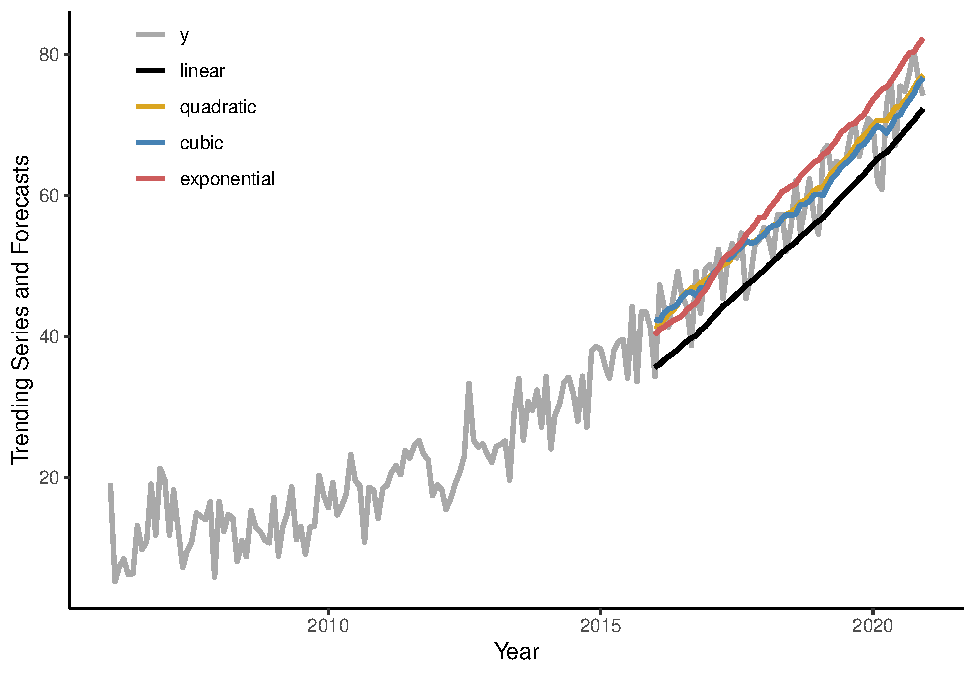
\includegraphics{forecasting_files/figure-latex/unnamed-chunk-61-1.pdf}

Calculate the RMSFE measures for each of the two forecasting methods.

\begin{Shaded}
\begin{Highlighting}[]
\NormalTok{dt[,}\StringTok{\textasciigrave{}}\AttributeTok{:=}\StringTok{\textasciigrave{}}\NormalTok{(}\AttributeTok{e\_t1=}\NormalTok{y}\SpecialCharTok{{-}}\NormalTok{t1,}\AttributeTok{e\_t2=}\NormalTok{y}\SpecialCharTok{{-}}\NormalTok{t2,}\AttributeTok{e\_t3=}\NormalTok{y}\SpecialCharTok{{-}}\NormalTok{t3,}\AttributeTok{e\_te=}\NormalTok{y}\SpecialCharTok{{-}}\NormalTok{te)]}

\NormalTok{rmsfe\_t1 }\OtherTok{\textless{}{-}} \FunctionTok{sqrt}\NormalTok{(}\FunctionTok{mean}\NormalTok{(dt}\SpecialCharTok{$}\NormalTok{e\_t1}\SpecialCharTok{\^{}}\DecValTok{2}\NormalTok{,}\AttributeTok{na.rm=}\NormalTok{T))}
\NormalTok{rmsfe\_t2 }\OtherTok{\textless{}{-}} \FunctionTok{sqrt}\NormalTok{(}\FunctionTok{mean}\NormalTok{(dt}\SpecialCharTok{$}\NormalTok{e\_t2}\SpecialCharTok{\^{}}\DecValTok{2}\NormalTok{,}\AttributeTok{na.rm=}\NormalTok{T))}
\NormalTok{rmsfe\_t3 }\OtherTok{\textless{}{-}} \FunctionTok{sqrt}\NormalTok{(}\FunctionTok{mean}\NormalTok{(dt}\SpecialCharTok{$}\NormalTok{e\_t3}\SpecialCharTok{\^{}}\DecValTok{2}\NormalTok{,}\AttributeTok{na.rm=}\NormalTok{T))}
\NormalTok{rmsfe\_te }\OtherTok{\textless{}{-}} \FunctionTok{sqrt}\NormalTok{(}\FunctionTok{mean}\NormalTok{(dt}\SpecialCharTok{$}\NormalTok{e\_te}\SpecialCharTok{\^{}}\DecValTok{2}\NormalTok{,}\AttributeTok{na.rm=}\NormalTok{T))}

\NormalTok{rmsfe\_t1}
\end{Highlighting}
\end{Shaded}

\begin{verbatim}
## [1] 6.151904
\end{verbatim}

\begin{Shaded}
\begin{Highlighting}[]
\NormalTok{rmsfe\_t2}
\end{Highlighting}
\end{Shaded}

\begin{verbatim}
## [1] 3.796861
\end{verbatim}

\begin{Shaded}
\begin{Highlighting}[]
\NormalTok{rmsfe\_t3}
\end{Highlighting}
\end{Shaded}

\begin{verbatim}
## [1] 3.906023
\end{verbatim}

\begin{Shaded}
\begin{Highlighting}[]
\NormalTok{rmsfe\_te}
\end{Highlighting}
\end{Shaded}

\begin{verbatim}
## [1] 5.132312
\end{verbatim}

\hypertarget{tutorial-5-seasonality}{%
\chapter*{Tutorial 5: Seasonality}\label{tutorial-5-seasonality}}
\addcontentsline{toc}{chapter}{Tutorial 5: Seasonality}

(this is a AR stuff, will need to move back)

In this tutorial, we will generate autocorrelated series, we will apply an information criterion to select a suitable autoregressive model, we will obtain and compare one-step-ahead forecasts from competing models using a rolling window procedure, and we will generate one set of multi-step forecasts to illustrate the convergence to unconditional mean of the series.

Let's generate a time series that follows an AR(2) process: \(y_{t} = 1.2y_{t-1}-0.3y_{t-2}+e_{t}\), where \(e_{t} \sim N(0,1)\), for \(t=1,\ldots,180\).

\begin{Shaded}
\begin{Highlighting}[]
\NormalTok{n }\OtherTok{\textless{}{-}} \DecValTok{180}

\FunctionTok{set.seed}\NormalTok{(}\DecValTok{7}\NormalTok{)}
\NormalTok{e }\OtherTok{\textless{}{-}} \FunctionTok{rnorm}\NormalTok{(n,}\DecValTok{0}\NormalTok{,}\DecValTok{1}\NormalTok{)}

\NormalTok{y }\OtherTok{\textless{}{-}} \FunctionTok{rep}\NormalTok{(}\ConstantTok{NA}\NormalTok{,n)}
\NormalTok{y[}\DecValTok{1}\NormalTok{] }\OtherTok{\textless{}{-}}\NormalTok{ e[}\DecValTok{1}\NormalTok{]}
\NormalTok{y[}\DecValTok{2}\NormalTok{] }\OtherTok{\textless{}{-}} \FloatTok{1.2}\SpecialCharTok{*}\NormalTok{y[}\DecValTok{1}\NormalTok{]}\SpecialCharTok{+}\NormalTok{e[}\DecValTok{2}\NormalTok{]}
\ControlFlowTok{for}\NormalTok{(i }\ControlFlowTok{in} \DecValTok{3}\SpecialCharTok{:}\NormalTok{n)\{}
\NormalTok{  y[i] }\OtherTok{\textless{}{-}} \FloatTok{1.2}\SpecialCharTok{*}\NormalTok{y[i}\DecValTok{{-}1}\NormalTok{]}\SpecialCharTok{{-}}\FloatTok{0.3}\SpecialCharTok{*}\NormalTok{y[i}\DecValTok{{-}2}\NormalTok{]}\SpecialCharTok{+}\NormalTok{e[i]}
\NormalTok{\}}
\end{Highlighting}
\end{Shaded}

Generate a vector of some arbitrary dates (e.g., suppose we deal with the monthly series beginning from January 2006), and store these along with \(y\) in a \textbf{data.table}, call it `dt.'

\begin{Shaded}
\begin{Highlighting}[]
\NormalTok{date }\OtherTok{\textless{}{-}} \FunctionTok{seq}\NormalTok{(}\FunctionTok{as.Date}\NormalTok{(}\StringTok{"2006{-}01{-}01"}\NormalTok{),}\AttributeTok{by=}\StringTok{"month"}\NormalTok{,}\AttributeTok{along.with=}\NormalTok{y)}

\NormalTok{dt }\OtherTok{\textless{}{-}} \FunctionTok{data.table}\NormalTok{(date,y)}
\end{Highlighting}
\end{Shaded}

Plot the realized time series using \textbf{ggplot} function.

\begin{Shaded}
\begin{Highlighting}[]
\FunctionTok{ggplot}\NormalTok{(dt,}\FunctionTok{aes}\NormalTok{(}\AttributeTok{x=}\NormalTok{date,}\AttributeTok{y=}\NormalTok{y))}\SpecialCharTok{+}
  \FunctionTok{geom\_line}\NormalTok{(}\AttributeTok{size=}\DecValTok{1}\NormalTok{)}\SpecialCharTok{+}
  \FunctionTok{labs}\NormalTok{(}\AttributeTok{x=}\StringTok{"Year"}\NormalTok{,}\AttributeTok{y=}\StringTok{"Trending Series"}\NormalTok{)}\SpecialCharTok{+}
  \FunctionTok{theme\_classic}\NormalTok{()}
\end{Highlighting}
\end{Shaded}

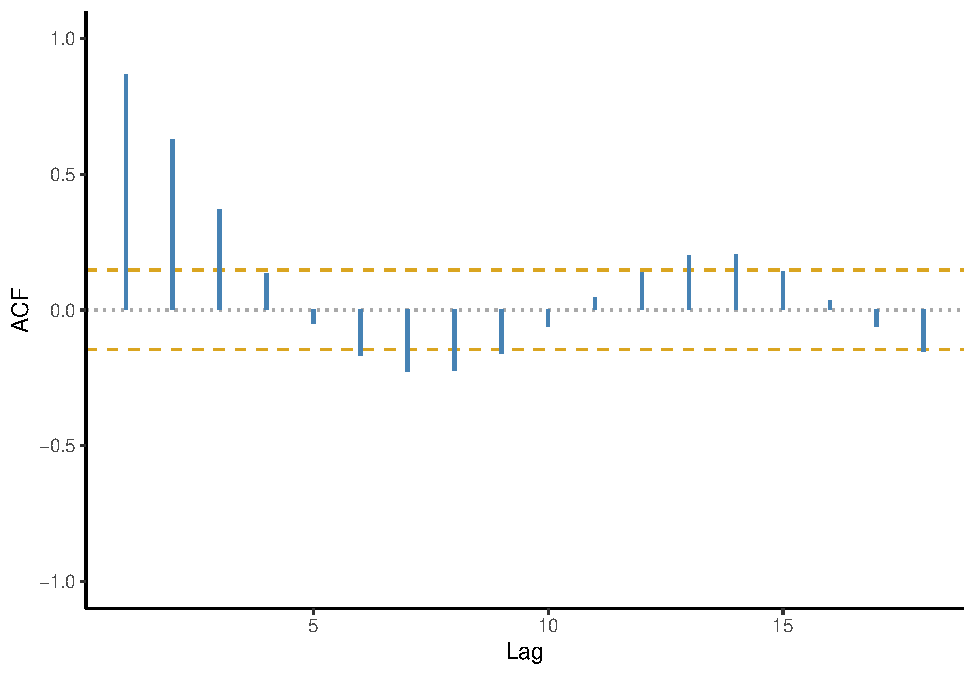
\includegraphics{forecasting_files/figure-latex/unnamed-chunk-66-1.pdf}

Generate and plot the autocorrelation function and the partial autocorrelation function for lags 1 through 18.

\begin{Shaded}
\begin{Highlighting}[]
\NormalTok{acf\_vec }\OtherTok{\textless{}{-}} \FunctionTok{c}\NormalTok{(}\FunctionTok{acf}\NormalTok{(dt}\SpecialCharTok{$}\NormalTok{y,}\AttributeTok{lag.max=}\DecValTok{18}\NormalTok{,}\AttributeTok{plot=}\NormalTok{F)}\SpecialCharTok{$}\NormalTok{acf[}\SpecialCharTok{{-}}\DecValTok{1}\NormalTok{])}
\NormalTok{pacf\_vec }\OtherTok{\textless{}{-}} \FunctionTok{c}\NormalTok{(}\FunctionTok{pacf}\NormalTok{(dt}\SpecialCharTok{$}\NormalTok{y,}\AttributeTok{lag.max=}\DecValTok{18}\NormalTok{,}\AttributeTok{plot=}\NormalTok{F)}\SpecialCharTok{$}\NormalTok{acf)}

\NormalTok{sd\_rho }\OtherTok{\textless{}{-}} \FunctionTok{sqrt}\NormalTok{(}\DecValTok{1}\SpecialCharTok{/}\NormalTok{n)}

\NormalTok{acf\_dt }\OtherTok{\textless{}{-}} \FunctionTok{data.table}\NormalTok{(}\AttributeTok{lags=}\DecValTok{1}\SpecialCharTok{:}\DecValTok{18}\NormalTok{,}\AttributeTok{acf=}\NormalTok{acf\_vec,}\AttributeTok{pacf=}\NormalTok{pacf\_vec)}

\FunctionTok{ggplot}\NormalTok{(acf\_dt,}\FunctionTok{aes}\NormalTok{(}\AttributeTok{x=}\NormalTok{lags,}\AttributeTok{y=}\NormalTok{acf)) }\SpecialCharTok{+}
  \FunctionTok{geom\_hline}\NormalTok{(}\AttributeTok{yintercept=}\DecValTok{0}\NormalTok{,}\AttributeTok{color=}\StringTok{"darkgray"}\NormalTok{,}\AttributeTok{linetype=}\DecValTok{3}\NormalTok{,}\AttributeTok{size=}\NormalTok{.}\DecValTok{5}\NormalTok{) }\SpecialCharTok{+}
  \FunctionTok{geom\_hline}\NormalTok{(}\AttributeTok{yintercept=}\FunctionTok{c}\NormalTok{(}\SpecialCharTok{{-}}\FloatTok{1.96}\SpecialCharTok{*}\NormalTok{sd\_rho,}\FloatTok{1.96}\SpecialCharTok{*}\NormalTok{sd\_rho),}\AttributeTok{color=}\StringTok{"goldenrod"}\NormalTok{,}\AttributeTok{linetype=}\DecValTok{2}\NormalTok{,}\AttributeTok{size=}\NormalTok{.}\DecValTok{6}\NormalTok{) }\SpecialCharTok{+}
  \FunctionTok{geom\_segment}\NormalTok{(}\FunctionTok{aes}\NormalTok{(}\AttributeTok{xend=}\NormalTok{lags,}\AttributeTok{yend=}\DecValTok{0}\NormalTok{),}\AttributeTok{color=}\StringTok{"steelblue"}\NormalTok{,}\AttributeTok{size=}\NormalTok{.}\DecValTok{8}\NormalTok{)}\SpecialCharTok{+}
  \FunctionTok{labs}\NormalTok{(}\AttributeTok{x=}\StringTok{"Lag"}\NormalTok{,}\AttributeTok{y=}\StringTok{"ACF"}\NormalTok{)}\SpecialCharTok{+}
  \FunctionTok{coord\_cartesian}\NormalTok{(}\AttributeTok{ylim=}\FunctionTok{c}\NormalTok{(}\SpecialCharTok{{-}}\DecValTok{1}\NormalTok{,}\DecValTok{1}\NormalTok{))}\SpecialCharTok{+}
  \FunctionTok{theme\_classic}\NormalTok{()}
\end{Highlighting}
\end{Shaded}

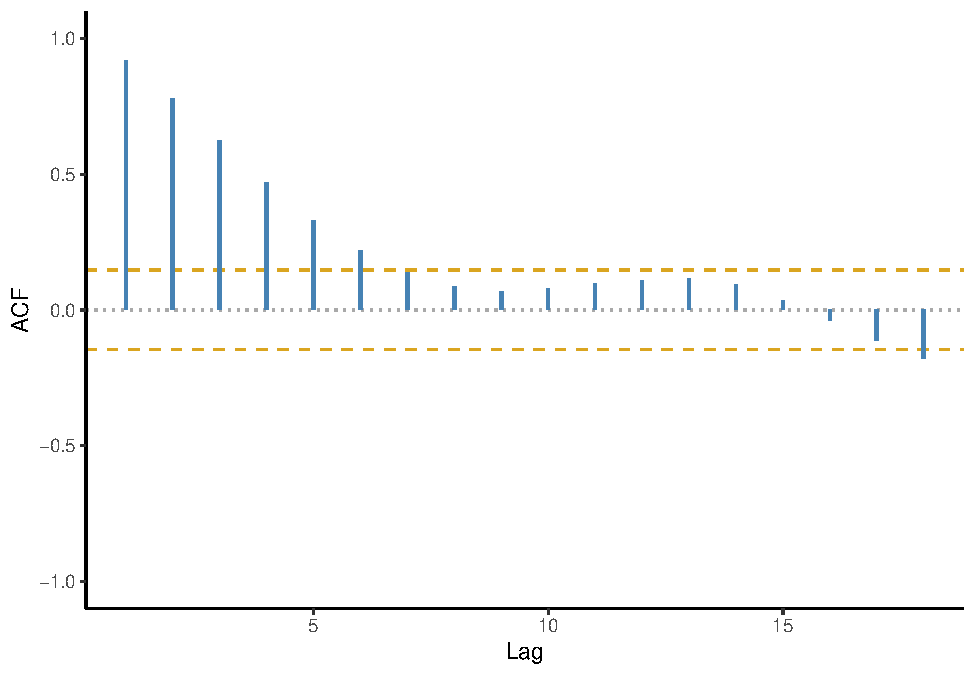
\includegraphics{forecasting_files/figure-latex/unnamed-chunk-67-1.pdf}

\begin{Shaded}
\begin{Highlighting}[]
\FunctionTok{ggplot}\NormalTok{(acf\_dt,}\FunctionTok{aes}\NormalTok{(}\AttributeTok{x=}\NormalTok{lags,}\AttributeTok{y=}\NormalTok{pacf)) }\SpecialCharTok{+}
  \FunctionTok{geom\_hline}\NormalTok{(}\AttributeTok{yintercept=}\DecValTok{0}\NormalTok{,}\AttributeTok{color=}\StringTok{"darkgray"}\NormalTok{,}\AttributeTok{linetype=}\DecValTok{3}\NormalTok{,}\AttributeTok{size=}\NormalTok{.}\DecValTok{5}\NormalTok{) }\SpecialCharTok{+}
  \FunctionTok{geom\_hline}\NormalTok{(}\AttributeTok{yintercept=}\FunctionTok{c}\NormalTok{(}\SpecialCharTok{{-}}\FloatTok{1.96}\SpecialCharTok{*}\NormalTok{sd\_rho,}\FloatTok{1.96}\SpecialCharTok{*}\NormalTok{sd\_rho),}\AttributeTok{color=}\StringTok{"goldenrod"}\NormalTok{,}\AttributeTok{linetype=}\DecValTok{2}\NormalTok{,}\AttributeTok{size=}\NormalTok{.}\DecValTok{6}\NormalTok{) }\SpecialCharTok{+}
  \FunctionTok{geom\_segment}\NormalTok{(}\FunctionTok{aes}\NormalTok{(}\AttributeTok{xend=}\NormalTok{lags,}\AttributeTok{yend=}\DecValTok{0}\NormalTok{),}\AttributeTok{color=}\StringTok{"steelblue"}\NormalTok{,}\AttributeTok{size=}\NormalTok{.}\DecValTok{8}\NormalTok{)}\SpecialCharTok{+}
  \FunctionTok{labs}\NormalTok{(}\AttributeTok{x=}\StringTok{"Lag"}\NormalTok{,}\AttributeTok{y=}\StringTok{"PACF"}\NormalTok{)}\SpecialCharTok{+}
  \FunctionTok{coord\_cartesian}\NormalTok{(}\AttributeTok{ylim=}\FunctionTok{c}\NormalTok{(}\SpecialCharTok{{-}}\DecValTok{1}\NormalTok{,}\DecValTok{1}\NormalTok{))}\SpecialCharTok{+}
  \FunctionTok{theme\_classic}\NormalTok{()}
\end{Highlighting}
\end{Shaded}

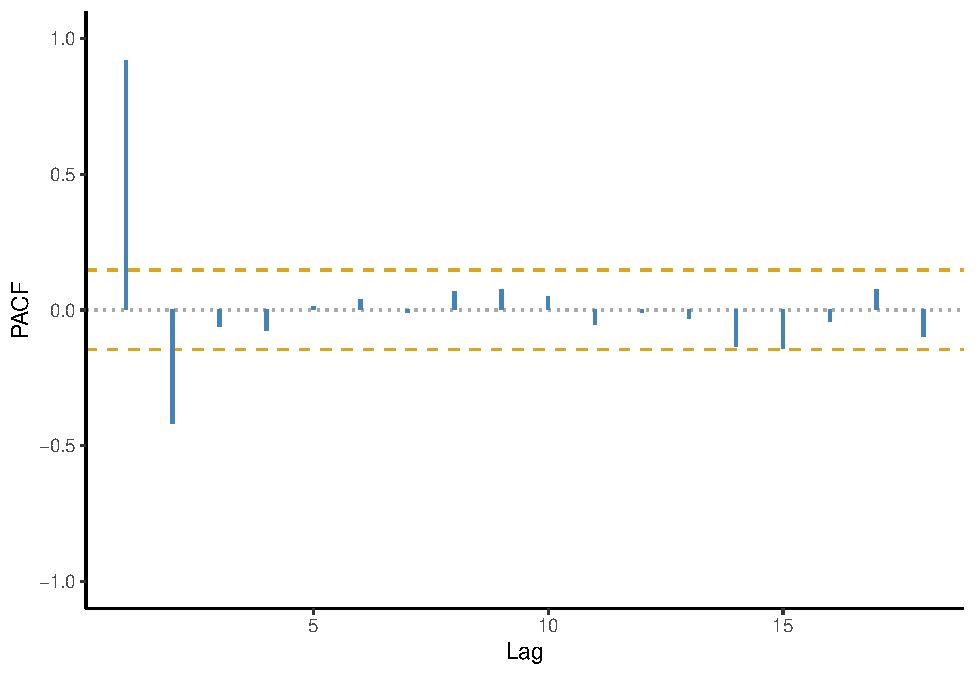
\includegraphics{forecasting_files/figure-latex/unnamed-chunk-67-2.pdf}

Calculate Akaike Information Criteria (AIC) and Schwarz Information Criteria (SIC) for AR(1), AR(2), AR(3), and AR(4) models, using all observations in the series, to decide on the optimal lag length.

\begin{Shaded}
\begin{Highlighting}[]
\NormalTok{dt[,}\StringTok{\textasciigrave{}}\AttributeTok{:=}\StringTok{\textasciigrave{}}\NormalTok{(}\AttributeTok{y\_l1=}\FunctionTok{shift}\NormalTok{(y),}\AttributeTok{y\_l2=}\FunctionTok{shift}\NormalTok{(y,}\DecValTok{2}\NormalTok{),}\AttributeTok{y\_l3=}\FunctionTok{shift}\NormalTok{(y,}\DecValTok{3}\NormalTok{),}\AttributeTok{y\_l4=}\FunctionTok{shift}\NormalTok{(y,}\DecValTok{4}\NormalTok{))]}

\CommentTok{\# get rid of the rows with NAs}
\NormalTok{dt }\OtherTok{\textless{}{-}}\NormalTok{ dt[}\FunctionTok{complete.cases}\NormalTok{(dt)]}

\NormalTok{IC\_dt }\OtherTok{\textless{}{-}} \FunctionTok{data.table}\NormalTok{(}\AttributeTok{lag=}\FunctionTok{c}\NormalTok{(}\DecValTok{1}\SpecialCharTok{:}\DecValTok{4}\NormalTok{),}\AttributeTok{AIC=}\ConstantTok{NA}\NormalTok{,}\AttributeTok{SIC=}\ConstantTok{NA}\NormalTok{)}

\ControlFlowTok{for}\NormalTok{(i }\ControlFlowTok{in} \DecValTok{1}\SpecialCharTok{:}\FunctionTok{nrow}\NormalTok{(IC\_dt))\{}
  
\NormalTok{  fmla }\OtherTok{\textless{}{-}} \FunctionTok{as.formula}\NormalTok{(}\FunctionTok{paste}\NormalTok{(}\StringTok{"y"}\NormalTok{,}\FunctionTok{paste0}\NormalTok{(}\StringTok{"y\_l"}\NormalTok{,}\FunctionTok{c}\NormalTok{(}\DecValTok{1}\SpecialCharTok{:}\NormalTok{i),}\AttributeTok{collapse=}\StringTok{"+"}\NormalTok{),}\AttributeTok{sep=}\StringTok{"\textasciitilde{}"}\NormalTok{))}
\NormalTok{  reg.ar }\OtherTok{\textless{}{-}} \FunctionTok{lm}\NormalTok{(fmla,}\AttributeTok{data=}\NormalTok{dt)}
  
\NormalTok{  IC\_dt}\SpecialCharTok{$}\NormalTok{AIC[i] }\OtherTok{\textless{}{-}} \FunctionTok{log}\NormalTok{(}\FunctionTok{crossprod}\NormalTok{(reg.ar}\SpecialCharTok{$}\NormalTok{residuals))}\SpecialCharTok{+}\DecValTok{2}\SpecialCharTok{*}\NormalTok{(i}\SpecialCharTok{+}\DecValTok{1}\NormalTok{)}\SpecialCharTok{/}\FunctionTok{nrow}\NormalTok{(dt)}
\NormalTok{  IC\_dt}\SpecialCharTok{$}\NormalTok{SIC[i] }\OtherTok{\textless{}{-}} \FunctionTok{log}\NormalTok{(}\FunctionTok{crossprod}\NormalTok{(reg.ar}\SpecialCharTok{$}\NormalTok{residuals))}\SpecialCharTok{+}\FunctionTok{log}\NormalTok{(}\FunctionTok{nrow}\NormalTok{(dt))}\SpecialCharTok{*}\NormalTok{(i}\SpecialCharTok{+}\DecValTok{1}\NormalTok{)}\SpecialCharTok{/}\FunctionTok{nrow}\NormalTok{(dt)}

\NormalTok{\}}

\NormalTok{IC\_dt}
\end{Highlighting}
\end{Shaded}

\begin{verbatim}
##    lag      AIC      SIC
## 1:   1 5.192156 5.228184
## 2:   2 5.011351 5.065393
## 3:   3 5.018687 5.090743
## 4:   4 5.024127 5.114198
\end{verbatim}

Generate a sequence of one-step-ahead forecasts from random walk, as well as AR(1), AR(2), and AR(3), using the rolling window scheme, where the first rolling window ranges from period 1 to period 120.

\begin{Shaded}
\begin{Highlighting}[]
\NormalTok{R }\OtherTok{\textless{}{-}} \DecValTok{120}
\NormalTok{P }\OtherTok{\textless{}{-}} \FunctionTok{nrow}\NormalTok{(dt)}\SpecialCharTok{{-}}\NormalTok{R}

\NormalTok{dt}\SpecialCharTok{$}\NormalTok{rw }\OtherTok{\textless{}{-}} \ConstantTok{NA}
\NormalTok{dt}\SpecialCharTok{$}\NormalTok{ar1 }\OtherTok{\textless{}{-}} \ConstantTok{NA}
\NormalTok{dt}\SpecialCharTok{$}\NormalTok{ar2 }\OtherTok{\textless{}{-}} \ConstantTok{NA}

\ControlFlowTok{for}\NormalTok{(i }\ControlFlowTok{in} \DecValTok{1}\SpecialCharTok{:}\NormalTok{P)\{}
\NormalTok{  dt}\SpecialCharTok{$}\NormalTok{rw[R}\SpecialCharTok{+}\NormalTok{i] }\OtherTok{\textless{}{-}}\NormalTok{ dt}\SpecialCharTok{$}\NormalTok{y[R}\DecValTok{{-}1}\SpecialCharTok{+}\NormalTok{i]}
  
\NormalTok{  ar1 }\OtherTok{\textless{}{-}} \FunctionTok{lm}\NormalTok{(y}\SpecialCharTok{\textasciitilde{}}\NormalTok{y\_l1,}\AttributeTok{data=}\NormalTok{dt[i}\SpecialCharTok{:}\NormalTok{(R}\DecValTok{{-}1}\SpecialCharTok{+}\NormalTok{i)])}
\NormalTok{  ar2 }\OtherTok{\textless{}{-}} \FunctionTok{lm}\NormalTok{(y}\SpecialCharTok{\textasciitilde{}}\NormalTok{y\_l1}\SpecialCharTok{+}\NormalTok{y\_l2,}\AttributeTok{data=}\NormalTok{dt[i}\SpecialCharTok{:}\NormalTok{(R}\DecValTok{{-}1}\SpecialCharTok{+}\NormalTok{i)])}
  
\NormalTok{  dt}\SpecialCharTok{$}\NormalTok{ar1[R}\SpecialCharTok{+}\NormalTok{i] }\OtherTok{\textless{}{-}}\NormalTok{ ar1}\SpecialCharTok{$}\NormalTok{coefficients[}\DecValTok{1}\NormalTok{]}\SpecialCharTok{+}\NormalTok{ar1}\SpecialCharTok{$}\NormalTok{coefficients[}\DecValTok{2}\NormalTok{]}\SpecialCharTok{*}\NormalTok{dt}\SpecialCharTok{$}\NormalTok{y[R}\DecValTok{{-}1}\SpecialCharTok{+}\NormalTok{i]}
\NormalTok{  dt}\SpecialCharTok{$}\NormalTok{ar2[R}\SpecialCharTok{+}\NormalTok{i] }\OtherTok{\textless{}{-}}\NormalTok{ ar2}\SpecialCharTok{$}\NormalTok{coefficients[}\DecValTok{1}\NormalTok{]}\SpecialCharTok{+}\NormalTok{ar2}\SpecialCharTok{$}\NormalTok{coefficients[}\DecValTok{2}\NormalTok{]}\SpecialCharTok{*}\NormalTok{dt}\SpecialCharTok{$}\NormalTok{y[R}\DecValTok{{-}1}\SpecialCharTok{+}\NormalTok{i]}\SpecialCharTok{+}\NormalTok{ar2}\SpecialCharTok{$}\NormalTok{coefficients[}\DecValTok{3}\NormalTok{]}\SpecialCharTok{*}\NormalTok{dt}\SpecialCharTok{$}\NormalTok{y[R}\DecValTok{{-}2}\SpecialCharTok{+}\NormalTok{i]}
\NormalTok{\}}
\end{Highlighting}
\end{Shaded}

Calculate the RMSFE measures for all considered models.

\begin{Shaded}
\begin{Highlighting}[]
\NormalTok{dt[,}\StringTok{\textasciigrave{}}\AttributeTok{:=}\StringTok{\textasciigrave{}}\NormalTok{(}\AttributeTok{rw\_e=}\NormalTok{y}\SpecialCharTok{{-}}\NormalTok{rw,}\AttributeTok{ar1\_e=}\NormalTok{y}\SpecialCharTok{{-}}\NormalTok{ar1,}\AttributeTok{ar2\_e=}\NormalTok{y}\SpecialCharTok{{-}}\NormalTok{ar2)]}

\NormalTok{rmsfe\_rw }\OtherTok{\textless{}{-}} \FunctionTok{sqrt}\NormalTok{(}\FunctionTok{mean}\NormalTok{(dt}\SpecialCharTok{$}\NormalTok{rw\_e}\SpecialCharTok{\^{}}\DecValTok{2}\NormalTok{,}\AttributeTok{na.rm=}\NormalTok{T))}
\NormalTok{rmsfe\_ar1 }\OtherTok{\textless{}{-}} \FunctionTok{sqrt}\NormalTok{(}\FunctionTok{mean}\NormalTok{(dt}\SpecialCharTok{$}\NormalTok{ar1\_e}\SpecialCharTok{\^{}}\DecValTok{2}\NormalTok{,}\AttributeTok{na.rm=}\NormalTok{T))}
\NormalTok{rmsfe\_ar2 }\OtherTok{\textless{}{-}} \FunctionTok{sqrt}\NormalTok{(}\FunctionTok{mean}\NormalTok{(dt}\SpecialCharTok{$}\NormalTok{ar2\_e}\SpecialCharTok{\^{}}\DecValTok{2}\NormalTok{,}\AttributeTok{na.rm=}\NormalTok{T))}

\NormalTok{rmsfe\_rw}
\end{Highlighting}
\end{Shaded}

\begin{verbatim}
## [1] 0.9569683
\end{verbatim}

\begin{Shaded}
\begin{Highlighting}[]
\NormalTok{rmsfe\_ar1}
\end{Highlighting}
\end{Shaded}

\begin{verbatim}
## [1] 0.9298374
\end{verbatim}

\begin{Shaded}
\begin{Highlighting}[]
\NormalTok{rmsfe\_ar2}
\end{Highlighting}
\end{Shaded}

\begin{verbatim}
## [1] 0.8901728
\end{verbatim}

Using the first rolling window as the information set, generate the multi-step-ahead forecast for the hold-out period.

\begin{Shaded}
\begin{Highlighting}[]
\NormalTok{dt[,}\StringTok{\textasciigrave{}}\AttributeTok{:=}\StringTok{\textasciigrave{}}\NormalTok{(}\AttributeTok{ar2\_multi=}\NormalTok{y)]}

\NormalTok{ar2 }\OtherTok{\textless{}{-}} \FunctionTok{lm}\NormalTok{(y}\SpecialCharTok{\textasciitilde{}}\NormalTok{y\_l1}\SpecialCharTok{+}\NormalTok{y\_l2,}\AttributeTok{data=}\NormalTok{dt[}\DecValTok{1}\SpecialCharTok{:}\NormalTok{R])}

\ControlFlowTok{for}\NormalTok{(i }\ControlFlowTok{in} \DecValTok{1}\SpecialCharTok{:}\NormalTok{P)\{}

\NormalTok{  dt}\SpecialCharTok{$}\NormalTok{ar2\_multi[R}\SpecialCharTok{+}\NormalTok{i] }\OtherTok{\textless{}{-}}\NormalTok{ ar2}\SpecialCharTok{$}\NormalTok{coefficients[}\DecValTok{1}\NormalTok{]}\SpecialCharTok{+}\NormalTok{ar2}\SpecialCharTok{$}\NormalTok{coefficients[}\DecValTok{2}\NormalTok{]}\SpecialCharTok{*}\NormalTok{dt}\SpecialCharTok{$}\NormalTok{ar2\_multi[R}\DecValTok{{-}1}\SpecialCharTok{+}\NormalTok{i]}\SpecialCharTok{+}\NormalTok{ar2}\SpecialCharTok{$}\NormalTok{coefficients[}\DecValTok{3}\NormalTok{]}\SpecialCharTok{*}\NormalTok{dt}\SpecialCharTok{$}\NormalTok{ar2\_multi[R}\DecValTok{{-}2}\SpecialCharTok{+}\NormalTok{i]}
  
\NormalTok{\}}

\NormalTok{dt[}\DecValTok{1}\SpecialCharTok{:}\NormalTok{R]}\SpecialCharTok{$}\NormalTok{ar2\_multi }\OtherTok{\textless{}{-}} \ConstantTok{NA}

\FunctionTok{ggplot}\NormalTok{(dt,}\FunctionTok{aes}\NormalTok{(}\AttributeTok{x=}\NormalTok{date))}\SpecialCharTok{+}
  \FunctionTok{geom\_line}\NormalTok{(}\FunctionTok{aes}\NormalTok{(}\AttributeTok{y=}\NormalTok{y),}\AttributeTok{color=}\StringTok{"darkgray"}\NormalTok{,}\AttributeTok{size=}\DecValTok{1}\NormalTok{)}\SpecialCharTok{+}
  \FunctionTok{geom\_line}\NormalTok{(}\FunctionTok{aes}\NormalTok{(}\AttributeTok{y=}\NormalTok{ar2\_multi),}\AttributeTok{color=}\StringTok{"steelblue"}\NormalTok{,}\AttributeTok{na.rm=}\NormalTok{T,}\AttributeTok{size=}\DecValTok{1}\NormalTok{,}\AttributeTok{linetype=}\DecValTok{5}\NormalTok{)}\SpecialCharTok{+}
  \FunctionTok{theme\_classic}\NormalTok{()}
\end{Highlighting}
\end{Shaded}

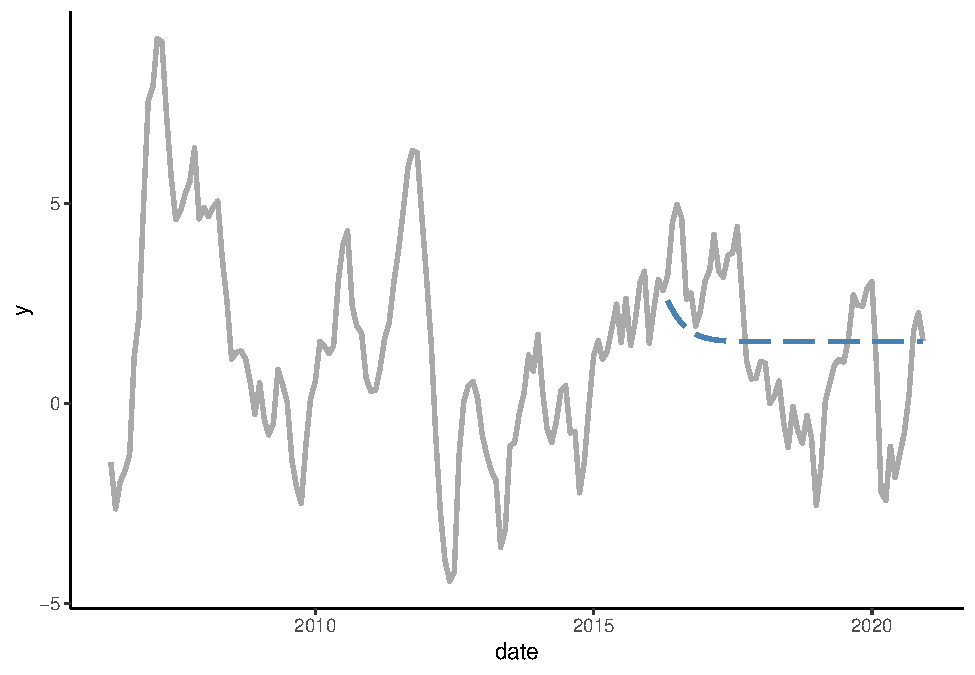
\includegraphics{forecasting_files/figure-latex/unnamed-chunk-71-1.pdf}

\hypertarget{tutorial-6-linear-autoregression}{%
\chapter*{Tutorial 6: Linear Autoregression}\label{tutorial-6-linear-autoregression}}
\addcontentsline{toc}{chapter}{Tutorial 6: Linear Autoregression}

(this is a VAR stuff, will need to move back)

In this tutorial, we will generate bivariate series, we will apply a system-wide information criterion to select a suitable vector autoregressive model, we will perform an in-sample test of Granger causality, we will obtain and compare one-step-ahead forecasts from competing models using a rolling window procedure, and in so doing we will investigate the evidence of Granger causality in an out-of-sample setting. To run the code, the \texttt{data.table} and \texttt{MASS} packages need to be installed and loaded.

Let's generate a two-dimensional vector of time series that follow a VAR(1) process of the following form: \[\begin{aligned}
x_{1,t} &= 0.3 + 0.7x_{1,t-1} + 0.1x_{2,t-1} + \varepsilon_{1,t} \\
x_{2,t} &= -0.2 + 0.9x_{1,t-1} + \varepsilon_{2,t}
\end{aligned}\] where \(\mathbf{e}_{t} \sim N(\mathbf{0},\Sigma)\), and where \(\Sigma\) is the covariance matrix of the residuals such that \(Cov(\varepsilon_{1,t},\varepsilon_{2,t}) = 0.3\) for all \(t=1,\ldots,180\). (Note: in the code, \(x_1\) is denoted by \(y\) and \(x_2\) is denoted by \(x\)).

\begin{Shaded}
\begin{Highlighting}[]
\NormalTok{n }\OtherTok{\textless{}{-}} \DecValTok{180}

\NormalTok{R }\OtherTok{\textless{}{-}} \FunctionTok{matrix}\NormalTok{(}\FunctionTok{c}\NormalTok{(}\DecValTok{1}\NormalTok{,}\FloatTok{0.3}\NormalTok{,}\FloatTok{0.3}\NormalTok{,}\DecValTok{1}\NormalTok{),}\AttributeTok{nrow=}\DecValTok{2}\NormalTok{,}\AttributeTok{ncol=}\DecValTok{2}\NormalTok{)}
\FunctionTok{set.seed}\NormalTok{(}\DecValTok{1}\NormalTok{)}
\NormalTok{e }\OtherTok{\textless{}{-}} \FunctionTok{mvrnorm}\NormalTok{(n,}\AttributeTok{mu=}\FunctionTok{c}\NormalTok{(}\DecValTok{0}\NormalTok{,}\DecValTok{0}\NormalTok{),}\AttributeTok{Sigma=}\NormalTok{R)}

\NormalTok{e\_y }\OtherTok{\textless{}{-}}\NormalTok{ e[,}\DecValTok{1}\NormalTok{]}
\NormalTok{e\_x }\OtherTok{\textless{}{-}}\NormalTok{ e[,}\DecValTok{2}\NormalTok{]}

\NormalTok{y }\OtherTok{\textless{}{-}} \FunctionTok{rep}\NormalTok{(}\ConstantTok{NA}\NormalTok{,n)}
\NormalTok{x }\OtherTok{\textless{}{-}} \FunctionTok{rep}\NormalTok{(}\ConstantTok{NA}\NormalTok{,n)}

\NormalTok{y[}\DecValTok{1}\NormalTok{] }\OtherTok{\textless{}{-}}\NormalTok{ e\_y[}\DecValTok{1}\NormalTok{]}
\NormalTok{x[}\DecValTok{1}\NormalTok{] }\OtherTok{\textless{}{-}}\NormalTok{ e\_x[}\DecValTok{1}\NormalTok{]}

\ControlFlowTok{for}\NormalTok{(i }\ControlFlowTok{in} \DecValTok{2}\SpecialCharTok{:}\NormalTok{n)\{}
\NormalTok{  y[i] }\OtherTok{\textless{}{-}} \FloatTok{0.3+0.7}\SpecialCharTok{*}\NormalTok{y[i}\DecValTok{{-}1}\NormalTok{]}\SpecialCharTok{+}\FloatTok{0.1}\SpecialCharTok{*}\NormalTok{x[i}\DecValTok{{-}1}\NormalTok{]}\SpecialCharTok{+}\NormalTok{e\_y[i]}
\NormalTok{  x[i] }\OtherTok{\textless{}{-}} \SpecialCharTok{{-}}\FloatTok{0.2+0.9}\SpecialCharTok{*}\NormalTok{x[i}\DecValTok{{-}1}\NormalTok{]}\SpecialCharTok{+}\NormalTok{e\_x[i]}
\NormalTok{\}}
\end{Highlighting}
\end{Shaded}

Generate a vector of some arbitrary dates (e.g., suppose we deal with the monthly series beginning from January 2006), and store these along with \(y\) in a \textbf{data.table}, call it `dt.'

\begin{Shaded}
\begin{Highlighting}[]
\NormalTok{date }\OtherTok{\textless{}{-}} \FunctionTok{seq}\NormalTok{(}\FunctionTok{as.Date}\NormalTok{(}\StringTok{"2006{-}01{-}01"}\NormalTok{),}\AttributeTok{by=}\StringTok{"month"}\NormalTok{,}\AttributeTok{along.with=}\NormalTok{y)}

\NormalTok{dt }\OtherTok{\textless{}{-}} \FunctionTok{data.table}\NormalTok{(date,y,x)}
\end{Highlighting}
\end{Shaded}

Plot the realized time series using \textbf{ggplot} function.

\begin{Shaded}
\begin{Highlighting}[]
\NormalTok{dt\_long }\OtherTok{\textless{}{-}} \FunctionTok{melt}\NormalTok{(dt,}\AttributeTok{id.vars=}\StringTok{"date"}\NormalTok{)}

\FunctionTok{ggplot}\NormalTok{(dt\_long,}\FunctionTok{aes}\NormalTok{(}\AttributeTok{x=}\NormalTok{date,}\AttributeTok{y=}\NormalTok{value,}\AttributeTok{color=}\NormalTok{variable,}\AttributeTok{linetype=}\NormalTok{variable))}\SpecialCharTok{+}
  \FunctionTok{geom\_line}\NormalTok{(}\AttributeTok{size=}\DecValTok{1}\NormalTok{)}\SpecialCharTok{+}
  \FunctionTok{scale\_color\_manual}\NormalTok{(}\AttributeTok{values=}\FunctionTok{c}\NormalTok{(}\StringTok{"darkgray"}\NormalTok{,}\StringTok{"steelblue"}\NormalTok{))}\SpecialCharTok{+}
  \FunctionTok{labs}\NormalTok{(}\AttributeTok{x=}\StringTok{"Year"}\NormalTok{,}\AttributeTok{y=}\StringTok{"Series"}\NormalTok{)}\SpecialCharTok{+}
  \FunctionTok{theme\_classic}\NormalTok{()}
\end{Highlighting}
\end{Shaded}

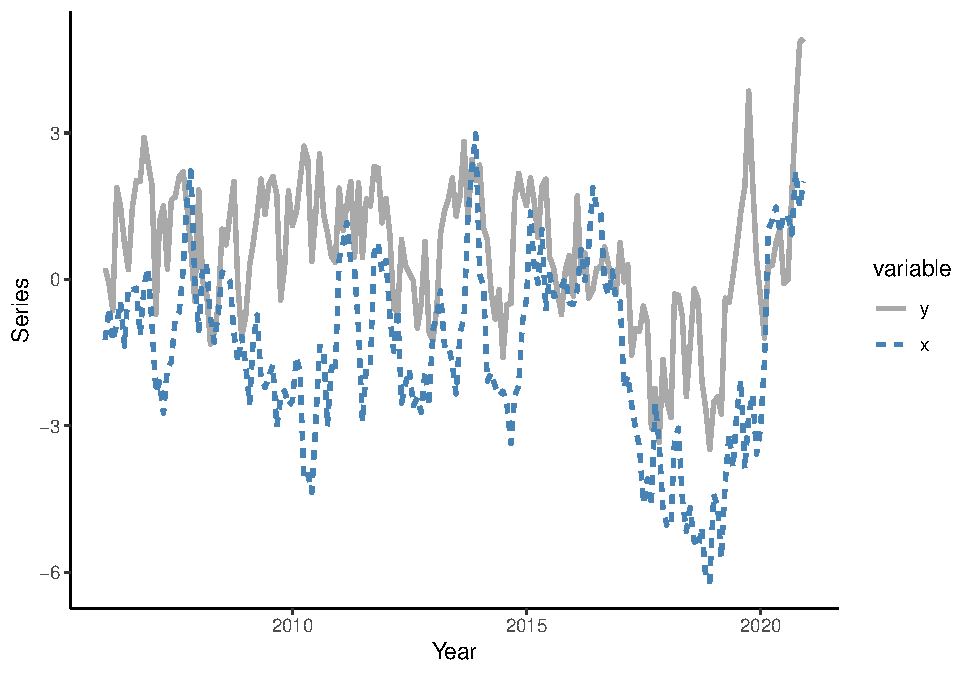
\includegraphics{forecasting_files/figure-latex/unnamed-chunk-75-1.pdf}

Estimate VAR(1) and VAR(2) by running regressions on each equation separately. Collect residuals and obtain system-wide AIC for each of the two models.

\begin{Shaded}
\begin{Highlighting}[]
\NormalTok{dt[,}\StringTok{\textasciigrave{}}\AttributeTok{:=}\StringTok{\textasciigrave{}}\NormalTok{(}\AttributeTok{y\_l1=}\FunctionTok{shift}\NormalTok{(y,}\DecValTok{1}\NormalTok{),}\AttributeTok{y\_l2=}\FunctionTok{shift}\NormalTok{(y,}\DecValTok{2}\NormalTok{),}\AttributeTok{x\_l1=}\FunctionTok{shift}\NormalTok{(x,}\DecValTok{1}\NormalTok{),}\AttributeTok{x\_l2=}\FunctionTok{shift}\NormalTok{(x,}\DecValTok{2}\NormalTok{))]}

\CommentTok{\# VAR(1)}
\NormalTok{p }\OtherTok{\textless{}{-}} \DecValTok{1}
\NormalTok{k }\OtherTok{\textless{}{-}} \DecValTok{2}

\NormalTok{var1y }\OtherTok{\textless{}{-}} \FunctionTok{lm}\NormalTok{(y}\SpecialCharTok{\textasciitilde{}}\NormalTok{y\_l1}\SpecialCharTok{+}\NormalTok{x\_l1,}\AttributeTok{data=}\NormalTok{dt)}
\NormalTok{var1x }\OtherTok{\textless{}{-}} \FunctionTok{lm}\NormalTok{(x}\SpecialCharTok{\textasciitilde{}}\NormalTok{y\_l1}\SpecialCharTok{+}\NormalTok{x\_l1,}\AttributeTok{data=}\NormalTok{dt)}

\NormalTok{var1r }\OtherTok{\textless{}{-}} \FunctionTok{cbind}\NormalTok{(var1y}\SpecialCharTok{$}\NormalTok{residuals,var1x}\SpecialCharTok{$}\NormalTok{residuals)}
\NormalTok{cov1r }\OtherTok{\textless{}{-}} \FunctionTok{crossprod}\NormalTok{(var1r)}\SpecialCharTok{/}\NormalTok{(}\FunctionTok{nrow}\NormalTok{(dt)}\SpecialCharTok{{-}}\NormalTok{(p}\SpecialCharTok{*}\NormalTok{k}\SpecialCharTok{\^{}}\DecValTok{2}\SpecialCharTok{+}\NormalTok{k))}

\NormalTok{AIC1 }\OtherTok{\textless{}{-}} \FunctionTok{log}\NormalTok{(}\FunctionTok{det}\NormalTok{(cov1r))}\SpecialCharTok{+}\DecValTok{2}\SpecialCharTok{*}\NormalTok{(p}\SpecialCharTok{*}\NormalTok{k}\SpecialCharTok{\^{}}\DecValTok{2}\SpecialCharTok{+}\NormalTok{k)}\SpecialCharTok{/}\FunctionTok{nrow}\NormalTok{(dt)}

\CommentTok{\# VAR(2)}
\NormalTok{p }\OtherTok{\textless{}{-}} \DecValTok{2}
\NormalTok{k }\OtherTok{\textless{}{-}} \DecValTok{2}

\NormalTok{var2y }\OtherTok{\textless{}{-}} \FunctionTok{lm}\NormalTok{(y}\SpecialCharTok{\textasciitilde{}}\NormalTok{y\_l1}\SpecialCharTok{+}\NormalTok{y\_l2}\SpecialCharTok{+}\NormalTok{x\_l1}\SpecialCharTok{+}\NormalTok{x\_l2,}\AttributeTok{data=}\NormalTok{dt)}
\NormalTok{var2x }\OtherTok{\textless{}{-}} \FunctionTok{lm}\NormalTok{(x}\SpecialCharTok{\textasciitilde{}}\NormalTok{y\_l1}\SpecialCharTok{+}\NormalTok{y\_l2}\SpecialCharTok{+}\NormalTok{x\_l1}\SpecialCharTok{+}\NormalTok{x\_l2,}\AttributeTok{data=}\NormalTok{dt)}

\NormalTok{var2r }\OtherTok{\textless{}{-}} \FunctionTok{cbind}\NormalTok{(var2y}\SpecialCharTok{$}\NormalTok{residuals,var2x}\SpecialCharTok{$}\NormalTok{residuals)}
\NormalTok{cov2r }\OtherTok{\textless{}{-}} \FunctionTok{crossprod}\NormalTok{(var2r)}\SpecialCharTok{/}\NormalTok{(}\FunctionTok{nrow}\NormalTok{(dt)}\SpecialCharTok{{-}}\NormalTok{(p}\SpecialCharTok{*}\NormalTok{k}\SpecialCharTok{\^{}}\DecValTok{2}\SpecialCharTok{+}\NormalTok{k))}

\NormalTok{AIC2 }\OtherTok{\textless{}{-}} \FunctionTok{log}\NormalTok{(}\FunctionTok{det}\NormalTok{(cov2r))}\SpecialCharTok{+}\DecValTok{2}\SpecialCharTok{*}\NormalTok{(p}\SpecialCharTok{*}\NormalTok{k}\SpecialCharTok{\^{}}\DecValTok{2}\SpecialCharTok{+}\NormalTok{k)}\SpecialCharTok{/}\FunctionTok{nrow}\NormalTok{(dt)}

\NormalTok{AIC1}
\end{Highlighting}
\end{Shaded}

\begin{verbatim}
## [1] -0.1270596
\end{verbatim}

\begin{Shaded}
\begin{Highlighting}[]
\NormalTok{AIC2}
\end{Highlighting}
\end{Shaded}

\begin{verbatim}
## [1] -0.047212
\end{verbatim}

Perfrom tests of (in-sample) Granger causality in each of the two models. Note, in the case of VAR(1), both t tests and F tests are applicable and they both provide identical inference. In the case of VAR(p), where \(p>1\), the only appropriate test is an F test for joint significance of the parameters associated with the lags of the potentially causal variable.

\begin{Shaded}
\begin{Highlighting}[]
\CommentTok{\# VAR(1)}

\DocumentationTok{\#\# t test}
\FunctionTok{summary}\NormalTok{(var1y)}
\end{Highlighting}
\end{Shaded}

\begin{verbatim}
## 
## Call:
## lm(formula = y ~ y_l1 + x_l1, data = dt)
## 
## Residuals:
##      Min       1Q   Median       3Q      Max 
## -2.32279 -0.63680 -0.00953  0.68826  2.63468 
## 
## Coefficients:
##             Estimate Std. Error t value Pr(>|t|)    
## (Intercept)  0.34926    0.11146   3.134  0.00202 ** 
## y_l1         0.68903    0.05877  11.725  < 2e-16 ***
## x_l1         0.11304    0.04509   2.507  0.01308 *  
## ---
## Signif. codes:  0 '***' 0.001 '**' 0.01 '*' 0.05 '.' 0.1 ' ' 1
## 
## Residual standard error: 0.976 on 176 degrees of freedom
##   (1 observation deleted due to missingness)
## Multiple R-squared:  0.5689, Adjusted R-squared:  0.564 
## F-statistic: 116.1 on 2 and 176 DF,  p-value: < 2.2e-16
\end{verbatim}

\begin{Shaded}
\begin{Highlighting}[]
\FunctionTok{summary}\NormalTok{(var1x)}
\end{Highlighting}
\end{Shaded}

\begin{verbatim}
## 
## Call:
## lm(formula = x ~ y_l1 + x_l1, data = dt)
## 
## Residuals:
##      Min       1Q   Median       3Q      Max 
## -2.38491 -0.68087  0.03216  0.66109  2.74762 
## 
## Coefficients:
##             Estimate Std. Error t value Pr(>|t|)    
## (Intercept) -0.22353    0.10805  -2.069    0.040 *  
## y_l1         0.05814    0.05697   1.021    0.309    
## x_l1         0.85285    0.04371  19.511   <2e-16 ***
## ---
## Signif. codes:  0 '***' 0.001 '**' 0.01 '*' 0.05 '.' 0.1 ' ' 1
## 
## Residual standard error: 0.9461 on 176 degrees of freedom
##   (1 observation deleted due to missingness)
## Multiple R-squared:  0.7536, Adjusted R-squared:  0.7508 
## F-statistic: 269.2 on 2 and 176 DF,  p-value: < 2.2e-16
\end{verbatim}

\begin{Shaded}
\begin{Highlighting}[]
\DocumentationTok{\#\# F test}
\NormalTok{ar1y }\OtherTok{\textless{}{-}} \FunctionTok{lm}\NormalTok{(y}\SpecialCharTok{\textasciitilde{}}\NormalTok{y\_l1,}\AttributeTok{data=}\NormalTok{dt)}
\NormalTok{ar1x }\OtherTok{\textless{}{-}} \FunctionTok{lm}\NormalTok{(x}\SpecialCharTok{\textasciitilde{}}\NormalTok{x\_l1,}\AttributeTok{data=}\NormalTok{dt)}

\FunctionTok{anova}\NormalTok{(var1y,ar1y)}
\end{Highlighting}
\end{Shaded}

\begin{verbatim}
## Analysis of Variance Table
## 
## Model 1: y ~ y_l1 + x_l1
## Model 2: y ~ y_l1
##   Res.Df    RSS Df Sum of Sq      F  Pr(>F)  
## 1    176 167.64                              
## 2    177 173.62 -1   -5.9866 6.2852 0.01308 *
## ---
## Signif. codes:  0 '***' 0.001 '**' 0.01 '*' 0.05 '.' 0.1 ' ' 1
\end{verbatim}

\begin{Shaded}
\begin{Highlighting}[]
\FunctionTok{anova}\NormalTok{(var1x,ar1x)}
\end{Highlighting}
\end{Shaded}

\begin{verbatim}
## Analysis of Variance Table
## 
## Model 1: x ~ y_l1 + x_l1
## Model 2: x ~ x_l1
##   Res.Df    RSS Df Sum of Sq      F Pr(>F)
## 1    176 157.54                           
## 2    177 158.47 -1  -0.93231 1.0416 0.3089
\end{verbatim}

\begin{Shaded}
\begin{Highlighting}[]
\DocumentationTok{\#\# VAR(2)}

\DocumentationTok{\#\#\# t test (no longer applicable to test GC)}
\FunctionTok{summary}\NormalTok{(var2y)}
\end{Highlighting}
\end{Shaded}

\begin{verbatim}
## 
## Call:
## lm(formula = y ~ y_l1 + y_l2 + x_l1 + x_l2, data = dt)
## 
## Residuals:
##      Min       1Q   Median       3Q      Max 
## -2.38088 -0.71387 -0.01504  0.72538  2.70511 
## 
## Coefficients:
##             Estimate Std. Error t value Pr(>|t|)    
## (Intercept)  0.32203    0.11775   2.735  0.00689 ** 
## y_l1         0.65954    0.07822   8.431  1.3e-14 ***
## y_l2         0.04964    0.07965   0.623  0.53397    
## x_l1         0.15919    0.08052   1.977  0.04962 *  
## x_l2        -0.05991    0.08104  -0.739  0.46080    
## ---
## Signif. codes:  0 '***' 0.001 '**' 0.01 '*' 0.05 '.' 0.1 ' ' 1
## 
## Residual standard error: 0.9816 on 173 degrees of freedom
##   (2 observations deleted due to missingness)
## Multiple R-squared:  0.5709, Adjusted R-squared:  0.561 
## F-statistic: 57.55 on 4 and 173 DF,  p-value: < 2.2e-16
\end{verbatim}

\begin{Shaded}
\begin{Highlighting}[]
\FunctionTok{summary}\NormalTok{(var2x)}
\end{Highlighting}
\end{Shaded}

\begin{verbatim}
## 
## Call:
## lm(formula = x ~ y_l1 + y_l2 + x_l1 + x_l2, data = dt)
## 
## Residuals:
##      Min       1Q   Median       3Q      Max 
## -2.37790 -0.64364  0.05401  0.67542  2.71827 
## 
## Coefficients:
##             Estimate Std. Error t value Pr(>|t|)    
## (Intercept) -0.24577    0.11419  -2.152   0.0328 *  
## y_l1         0.03070    0.07586   0.405   0.6862    
## y_l2         0.04486    0.07724   0.581   0.5621    
## x_l1         0.86196    0.07809  11.039   <2e-16 ***
## x_l2        -0.01627    0.07859  -0.207   0.8362    
## ---
## Signif. codes:  0 '***' 0.001 '**' 0.01 '*' 0.05 '.' 0.1 ' ' 1
## 
## Residual standard error: 0.9519 on 173 degrees of freedom
##   (2 observations deleted due to missingness)
## Multiple R-squared:  0.7546, Adjusted R-squared:  0.7489 
## F-statistic:   133 on 4 and 173 DF,  p-value: < 2.2e-16
\end{verbatim}

\begin{Shaded}
\begin{Highlighting}[]
\DocumentationTok{\#\#\# F test}
\NormalTok{ar2y }\OtherTok{\textless{}{-}} \FunctionTok{lm}\NormalTok{(y}\SpecialCharTok{\textasciitilde{}}\NormalTok{y\_l1}\SpecialCharTok{+}\NormalTok{y\_l2,}\AttributeTok{data=}\NormalTok{dt)}
\NormalTok{ar2x }\OtherTok{\textless{}{-}} \FunctionTok{lm}\NormalTok{(x}\SpecialCharTok{\textasciitilde{}}\NormalTok{x\_l1}\SpecialCharTok{+}\NormalTok{x\_l2,}\AttributeTok{data=}\NormalTok{dt)}

\FunctionTok{anova}\NormalTok{(var2y,ar2y)}
\end{Highlighting}
\end{Shaded}

\begin{verbatim}
## Analysis of Variance Table
## 
## Model 1: y ~ y_l1 + y_l2 + x_l1 + x_l2
## Model 2: y ~ y_l1 + y_l2
##   Res.Df    RSS Df Sum of Sq      F  Pr(>F)  
## 1    173 166.68                              
## 2    175 172.78 -2   -6.0971 3.1641 0.04471 *
## ---
## Signif. codes:  0 '***' 0.001 '**' 0.01 '*' 0.05 '.' 0.1 ' ' 1
\end{verbatim}

\begin{Shaded}
\begin{Highlighting}[]
\FunctionTok{anova}\NormalTok{(var2x,ar2x)}
\end{Highlighting}
\end{Shaded}

\begin{verbatim}
## Analysis of Variance Table
## 
## Model 1: x ~ y_l1 + y_l2 + x_l1 + x_l2
## Model 2: x ~ x_l1 + x_l2
##   Res.Df    RSS Df Sum of Sq      F Pr(>F)
## 1    173 156.76                           
## 2    175 158.03 -2   -1.2729 0.7024 0.4968
\end{verbatim}

Generate a sequence of one-step-ahead forecasts from VAR(1) using the rolling window scheme, where the first rolling window ranges from period 1 to period 120.

\begin{Shaded}
\begin{Highlighting}[]
\NormalTok{R }\OtherTok{\textless{}{-}} \DecValTok{120}
\NormalTok{P }\OtherTok{\textless{}{-}} \FunctionTok{nrow}\NormalTok{(dt)}\SpecialCharTok{{-}}\NormalTok{R}

\NormalTok{dt}\SpecialCharTok{$}\NormalTok{ar1y }\OtherTok{\textless{}{-}} \ConstantTok{NA}
\NormalTok{dt}\SpecialCharTok{$}\NormalTok{ar1x }\OtherTok{\textless{}{-}} \ConstantTok{NA}
\NormalTok{dt}\SpecialCharTok{$}\NormalTok{var1y }\OtherTok{\textless{}{-}} \ConstantTok{NA}
\NormalTok{dt}\SpecialCharTok{$}\NormalTok{var1x }\OtherTok{\textless{}{-}} \ConstantTok{NA}

\ControlFlowTok{for}\NormalTok{(i }\ControlFlowTok{in} \DecValTok{1}\SpecialCharTok{:}\NormalTok{P)\{}
  
\NormalTok{  ar1y }\OtherTok{\textless{}{-}} \FunctionTok{lm}\NormalTok{(y}\SpecialCharTok{\textasciitilde{}}\NormalTok{y\_l1,}\AttributeTok{data=}\NormalTok{dt[i}\SpecialCharTok{:}\NormalTok{(R}\DecValTok{{-}1}\SpecialCharTok{+}\NormalTok{i)])}
\NormalTok{  ar1x }\OtherTok{\textless{}{-}} \FunctionTok{lm}\NormalTok{(x}\SpecialCharTok{\textasciitilde{}}\NormalTok{x\_l1,}\AttributeTok{data=}\NormalTok{dt[i}\SpecialCharTok{:}\NormalTok{(R}\DecValTok{{-}1}\SpecialCharTok{+}\NormalTok{i)])}
  
\NormalTok{  var1y }\OtherTok{\textless{}{-}} \FunctionTok{lm}\NormalTok{(y}\SpecialCharTok{\textasciitilde{}}\NormalTok{y\_l1}\SpecialCharTok{+}\NormalTok{x\_l1,}\AttributeTok{data=}\NormalTok{dt[i}\SpecialCharTok{:}\NormalTok{(R}\DecValTok{{-}1}\SpecialCharTok{+}\NormalTok{i)])}
\NormalTok{  var1x }\OtherTok{\textless{}{-}} \FunctionTok{lm}\NormalTok{(x}\SpecialCharTok{\textasciitilde{}}\NormalTok{y\_l1}\SpecialCharTok{+}\NormalTok{x\_l1,}\AttributeTok{data=}\NormalTok{dt[i}\SpecialCharTok{:}\NormalTok{(R}\DecValTok{{-}1}\SpecialCharTok{+}\NormalTok{i)])}
  
\NormalTok{  dt}\SpecialCharTok{$}\NormalTok{ar1y[R}\SpecialCharTok{+}\NormalTok{i] }\OtherTok{\textless{}{-}}\NormalTok{ ar1y}\SpecialCharTok{$}\NormalTok{coefficients[}\DecValTok{1}\NormalTok{]}\SpecialCharTok{+}\NormalTok{ar1y}\SpecialCharTok{$}\NormalTok{coefficients[}\DecValTok{2}\NormalTok{]}\SpecialCharTok{*}\NormalTok{dt}\SpecialCharTok{$}\NormalTok{y[R}\DecValTok{{-}1}\SpecialCharTok{+}\NormalTok{i]}
\NormalTok{  dt}\SpecialCharTok{$}\NormalTok{ar1x[R}\SpecialCharTok{+}\NormalTok{i] }\OtherTok{\textless{}{-}}\NormalTok{ ar1x}\SpecialCharTok{$}\NormalTok{coefficients[}\DecValTok{1}\NormalTok{]}\SpecialCharTok{+}\NormalTok{ar1x}\SpecialCharTok{$}\NormalTok{coefficients[}\DecValTok{2}\NormalTok{]}\SpecialCharTok{*}\NormalTok{dt}\SpecialCharTok{$}\NormalTok{x[R}\DecValTok{{-}1}\SpecialCharTok{+}\NormalTok{i]}
  
\NormalTok{  dt}\SpecialCharTok{$}\NormalTok{var1y[R}\SpecialCharTok{+}\NormalTok{i] }\OtherTok{\textless{}{-}}\NormalTok{ var1y}\SpecialCharTok{$}\NormalTok{coefficients[}\DecValTok{1}\NormalTok{]}\SpecialCharTok{+}\NormalTok{var1y}\SpecialCharTok{$}\NormalTok{coefficients[}\DecValTok{2}\NormalTok{]}\SpecialCharTok{*}\NormalTok{dt}\SpecialCharTok{$}\NormalTok{y[R}\DecValTok{{-}1}\SpecialCharTok{+}\NormalTok{i]}\SpecialCharTok{+}\NormalTok{var1y}\SpecialCharTok{$}\NormalTok{coefficients[}\DecValTok{3}\NormalTok{]}\SpecialCharTok{*}\NormalTok{dt}\SpecialCharTok{$}\NormalTok{x[R}\DecValTok{{-}1}\SpecialCharTok{+}\NormalTok{i]}
\NormalTok{  dt}\SpecialCharTok{$}\NormalTok{var1x[R}\SpecialCharTok{+}\NormalTok{i] }\OtherTok{\textless{}{-}}\NormalTok{ var1x}\SpecialCharTok{$}\NormalTok{coefficients[}\DecValTok{1}\NormalTok{]}\SpecialCharTok{+}\NormalTok{var1x}\SpecialCharTok{$}\NormalTok{coefficients[}\DecValTok{2}\NormalTok{]}\SpecialCharTok{*}\NormalTok{dt}\SpecialCharTok{$}\NormalTok{y[R}\DecValTok{{-}1}\SpecialCharTok{+}\NormalTok{i]}\SpecialCharTok{+}\NormalTok{var1x}\SpecialCharTok{$}\NormalTok{coefficients[}\DecValTok{3}\NormalTok{]}\SpecialCharTok{*}\NormalTok{dt}\SpecialCharTok{$}\NormalTok{x[R}\DecValTok{{-}1}\SpecialCharTok{+}\NormalTok{i]}
  
\NormalTok{\}}
\end{Highlighting}
\end{Shaded}

Calculate the RMSFE measures for restricted and unrestricted models, and compare those to each other to make a suggestion about out-of-sample Granger causality.

\begin{Shaded}
\begin{Highlighting}[]
\NormalTok{dt[,}\StringTok{\textasciigrave{}}\AttributeTok{:=}\StringTok{\textasciigrave{}}\NormalTok{(}\AttributeTok{ar1y\_e=}\NormalTok{y}\SpecialCharTok{{-}}\NormalTok{ar1y,}\AttributeTok{ar1x\_e=}\NormalTok{x}\SpecialCharTok{{-}}\NormalTok{ar1x,}\AttributeTok{var1y\_e=}\NormalTok{y}\SpecialCharTok{{-}}\NormalTok{var1y,}\AttributeTok{var1x\_e=}\NormalTok{x}\SpecialCharTok{{-}}\NormalTok{var1x)]}

\CommentTok{\# calculate RMSFE for restructed and unrestricted models}
\NormalTok{rmsfe\_yr }\OtherTok{\textless{}{-}} \FunctionTok{sqrt}\NormalTok{(}\FunctionTok{mean}\NormalTok{(dt}\SpecialCharTok{$}\NormalTok{ar1y\_e}\SpecialCharTok{\^{}}\DecValTok{2}\NormalTok{,}\AttributeTok{na.rm=}\NormalTok{T))}
\NormalTok{rmsfe\_yu }\OtherTok{\textless{}{-}} \FunctionTok{sqrt}\NormalTok{(}\FunctionTok{mean}\NormalTok{(dt}\SpecialCharTok{$}\NormalTok{var1y\_e}\SpecialCharTok{\^{}}\DecValTok{2}\NormalTok{,}\AttributeTok{na.rm=}\NormalTok{T))}

\NormalTok{rmsfe\_xr }\OtherTok{\textless{}{-}} \FunctionTok{sqrt}\NormalTok{(}\FunctionTok{mean}\NormalTok{(dt}\SpecialCharTok{$}\NormalTok{ar1x\_e}\SpecialCharTok{\^{}}\DecValTok{2}\NormalTok{,}\AttributeTok{na.rm=}\NormalTok{T))}
\NormalTok{rmsfe\_xu }\OtherTok{\textless{}{-}} \FunctionTok{sqrt}\NormalTok{(}\FunctionTok{mean}\NormalTok{(dt}\SpecialCharTok{$}\NormalTok{var1x\_e}\SpecialCharTok{\^{}}\DecValTok{2}\NormalTok{,}\AttributeTok{na.rm=}\NormalTok{T))}

\NormalTok{rmsfe\_yr}
\end{Highlighting}
\end{Shaded}

\begin{verbatim}
## [1] 1.134867
\end{verbatim}

\begin{Shaded}
\begin{Highlighting}[]
\NormalTok{rmsfe\_yu}
\end{Highlighting}
\end{Shaded}

\begin{verbatim}
## [1] 1.104268
\end{verbatim}

\begin{Shaded}
\begin{Highlighting}[]
\NormalTok{rmsfe\_xr}
\end{Highlighting}
\end{Shaded}

\begin{verbatim}
## [1] 1.00908
\end{verbatim}

\begin{Shaded}
\begin{Highlighting}[]
\NormalTok{rmsfe\_xu}
\end{Highlighting}
\end{Shaded}

\begin{verbatim}
## [1] 1.011653
\end{verbatim}

\hypertarget{tutorial-7-vector-autoregression}{%
\chapter*{Tutorial 7: Vector Autoregression}\label{tutorial-7-vector-autoregression}}
\addcontentsline{toc}{chapter}{Tutorial 7: Vector Autoregression}

(this is a threshold stuff, will need to move back)

In this tutorial, we will generate regime-dependent series, we will apply a grid-search method to obtain the threshold parameter, we will obtain and compare one-step-ahead forecasts from competing models using a rolling window procedure, and we will apply bootstrap resampling method to generate multi-step-ahead forecasts from a threshold regression. To run the code, the \texttt{data.table} and \texttt{ggplot2} packages need to be installed and loaded.

Let's generate a time series that follow a TAR(2) process of the following form:
\[y_t = \left\{\begin{array}
{ll}
y_{t-1} + \varepsilon_t & \text{if}~~y_{t-1}\ge0 \\
1.2y_{t-1}-0.3y_{t-2} + \varepsilon_t & \text{if}~~y_{t-1} < 0
\end{array}\right.
\]
where \(e_{t} \sim N(0,\sigma^2)\). This suggests that the time series follow the unit root process if the lagged dependent variable is non-negative, otherwise the time series is a mean-reverting AR(2) process.

\begin{Shaded}
\begin{Highlighting}[]
\NormalTok{n }\OtherTok{\textless{}{-}} \DecValTok{360}

\FunctionTok{set.seed}\NormalTok{(}\DecValTok{6}\NormalTok{)}
\NormalTok{e }\OtherTok{\textless{}{-}} \FunctionTok{rnorm}\NormalTok{(n,}\DecValTok{0}\NormalTok{,}\DecValTok{1}\NormalTok{)}

\NormalTok{y }\OtherTok{\textless{}{-}} \FunctionTok{rep}\NormalTok{(}\ConstantTok{NA}\NormalTok{,n)}
\NormalTok{y[}\DecValTok{1}\NormalTok{] }\OtherTok{\textless{}{-}}\NormalTok{ e[}\DecValTok{1}\NormalTok{]}
\ControlFlowTok{if}\NormalTok{(y[}\DecValTok{1}\NormalTok{]}\SpecialCharTok{\textgreater{}=}\DecValTok{0}\NormalTok{)\{}
\NormalTok{  y[}\DecValTok{2}\NormalTok{] }\OtherTok{\textless{}{-}}  \FloatTok{1.0}\SpecialCharTok{*}\NormalTok{y[}\DecValTok{1}\NormalTok{]}\SpecialCharTok{+}\NormalTok{e[}\DecValTok{2}\NormalTok{]}
\NormalTok{\}}\ControlFlowTok{else}\NormalTok{\{}
\NormalTok{  y[}\DecValTok{2}\NormalTok{] }\OtherTok{\textless{}{-}} \FloatTok{1.2}\SpecialCharTok{*}\NormalTok{y[}\DecValTok{1}\NormalTok{]}\SpecialCharTok{+}\NormalTok{e[}\DecValTok{2}\NormalTok{]}
\NormalTok{\}}

\ControlFlowTok{for}\NormalTok{(i }\ControlFlowTok{in} \DecValTok{3}\SpecialCharTok{:}\NormalTok{n)\{}
  \ControlFlowTok{if}\NormalTok{(y[i}\DecValTok{{-}1}\NormalTok{]}\SpecialCharTok{\textgreater{}=}\DecValTok{0}\NormalTok{)\{}
\NormalTok{    y[i] }\OtherTok{\textless{}{-}}  \FloatTok{1.0}\SpecialCharTok{*}\NormalTok{y[i}\DecValTok{{-}1}\NormalTok{]}\SpecialCharTok{+}\NormalTok{e[i]}
\NormalTok{  \}}\ControlFlowTok{else}\NormalTok{\{}
\NormalTok{    y[i] }\OtherTok{\textless{}{-}} \FloatTok{1.2}\SpecialCharTok{*}\NormalTok{y[i}\DecValTok{{-}1}\NormalTok{]}\SpecialCharTok{{-}}\FloatTok{0.3}\SpecialCharTok{*}\NormalTok{y[i}\DecValTok{{-}2}\NormalTok{]}\SpecialCharTok{+}\NormalTok{e[i]}
\NormalTok{  \}}
\NormalTok{\}}
\end{Highlighting}
\end{Shaded}

Generate a vector of some arbitrary dates (e.g., suppose we deal with the monthly series beginning from January 1991), and store these along with \(y\) in a \textbf{data.table}, call it `dt.'

\begin{Shaded}
\begin{Highlighting}[]
\NormalTok{date }\OtherTok{\textless{}{-}} \FunctionTok{seq}\NormalTok{(}\FunctionTok{as.Date}\NormalTok{(}\StringTok{"1991{-}01{-}01"}\NormalTok{),}\AttributeTok{by=}\StringTok{"month"}\NormalTok{,}\AttributeTok{along.with=}\NormalTok{y)}

\NormalTok{dt }\OtherTok{\textless{}{-}} \FunctionTok{data.table}\NormalTok{(date,y)}
\end{Highlighting}
\end{Shaded}

Plot the realized time series using \textbf{ggplot} function.

\begin{Shaded}
\begin{Highlighting}[]
\FunctionTok{ggplot}\NormalTok{(dt,}\FunctionTok{aes}\NormalTok{(}\AttributeTok{x=}\NormalTok{date,}\AttributeTok{y=}\NormalTok{y))}\SpecialCharTok{+}
  \FunctionTok{geom\_line}\NormalTok{(}\AttributeTok{size=}\DecValTok{1}\NormalTok{)}\SpecialCharTok{+}
  \FunctionTok{labs}\NormalTok{(}\AttributeTok{x=}\StringTok{"Year"}\NormalTok{,}\AttributeTok{y=}\StringTok{"Series"}\NormalTok{)}\SpecialCharTok{+}
  \FunctionTok{theme\_classic}\NormalTok{()}
\end{Highlighting}
\end{Shaded}

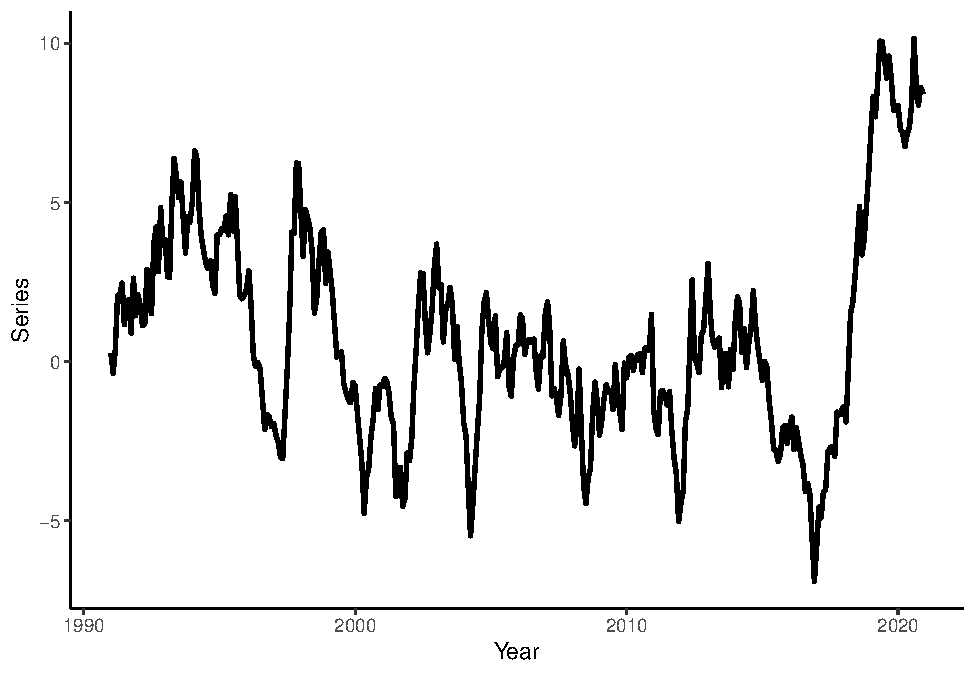
\includegraphics{forecasting_files/figure-latex/unnamed-chunk-83-1.pdf}

Decide on the optimal lag length based on AIC.

\begin{Shaded}
\begin{Highlighting}[]
\NormalTok{dt[,}\StringTok{\textasciigrave{}}\AttributeTok{:=}\StringTok{\textasciigrave{}}\NormalTok{(}\AttributeTok{y\_l1=}\FunctionTok{shift}\NormalTok{(y),}\AttributeTok{y\_l2=}\FunctionTok{shift}\NormalTok{(y,}\DecValTok{2}\NormalTok{),}\AttributeTok{y\_l3=}\FunctionTok{shift}\NormalTok{(y,}\DecValTok{3}\NormalTok{),}\AttributeTok{y\_l4=}\FunctionTok{shift}\NormalTok{(y,}\DecValTok{4}\NormalTok{))]}
\NormalTok{dt }\OtherTok{\textless{}{-}}\NormalTok{ dt[}\FunctionTok{complete.cases}\NormalTok{(dt)]}

\NormalTok{IC\_dt }\OtherTok{\textless{}{-}} \FunctionTok{data.table}\NormalTok{(}\AttributeTok{lag=}\FunctionTok{c}\NormalTok{(}\DecValTok{1}\SpecialCharTok{:}\DecValTok{4}\NormalTok{),}\AttributeTok{AIC=}\FunctionTok{as.numeric}\NormalTok{(}\ConstantTok{NA}\NormalTok{),}\AttributeTok{SIC=}\FunctionTok{as.numeric}\NormalTok{(}\ConstantTok{NA}\NormalTok{))}

\ControlFlowTok{for}\NormalTok{(i }\ControlFlowTok{in} \DecValTok{1}\SpecialCharTok{:}\FunctionTok{nrow}\NormalTok{(IC\_dt))\{}
  
\NormalTok{  fmla }\OtherTok{\textless{}{-}} \FunctionTok{as.formula}\NormalTok{(}\FunctionTok{paste}\NormalTok{(}\StringTok{"y"}\NormalTok{,}\FunctionTok{paste0}\NormalTok{(}\StringTok{"y\_l"}\NormalTok{,}\FunctionTok{c}\NormalTok{(}\DecValTok{1}\SpecialCharTok{:}\NormalTok{i),}\AttributeTok{collapse=}\StringTok{"+"}\NormalTok{),}\AttributeTok{sep=}\StringTok{"\textasciitilde{}"}\NormalTok{))}
\NormalTok{  reg.ar }\OtherTok{\textless{}{-}} \FunctionTok{lm}\NormalTok{(fmla,}\AttributeTok{data=}\NormalTok{dt)}
  
\NormalTok{  IC\_dt}\SpecialCharTok{$}\NormalTok{AIC[i] }\OtherTok{\textless{}{-}} \FunctionTok{log}\NormalTok{(}\FunctionTok{crossprod}\NormalTok{(reg.ar}\SpecialCharTok{$}\NormalTok{residuals))}\SpecialCharTok{+}\DecValTok{2}\SpecialCharTok{*}\NormalTok{(i}\SpecialCharTok{+}\DecValTok{1}\NormalTok{)}\SpecialCharTok{/}\FunctionTok{nrow}\NormalTok{(dt)}
\NormalTok{  IC\_dt}\SpecialCharTok{$}\NormalTok{SIC[i] }\OtherTok{\textless{}{-}} \FunctionTok{log}\NormalTok{(}\FunctionTok{crossprod}\NormalTok{(reg.ar}\SpecialCharTok{$}\NormalTok{residuals))}\SpecialCharTok{+}\FunctionTok{log}\NormalTok{(}\FunctionTok{nrow}\NormalTok{(dt))}\SpecialCharTok{*}\NormalTok{(i}\SpecialCharTok{+}\DecValTok{1}\NormalTok{)}\SpecialCharTok{/}\FunctionTok{nrow}\NormalTok{(dt)}

\NormalTok{\}}

\NormalTok{IC\_dt}
\end{Highlighting}
\end{Shaded}

\begin{verbatim}
##    lag      AIC      SIC
## 1:   1 5.822589 5.844358
## 2:   2 5.821342 5.853996
## 3:   3 5.826916 5.870454
## 4:   4 5.832294 5.886717
\end{verbatim}

We now need to get an estimate of the threshold parameter (i.e., the value at which the switch between the regimes happens). For that, we perform a grid-search routine. We will consider a range of candidate thresholds that are within 10th and 90th percentile of the lagged dependent variable. For each candidate threshold, we will run an OLS and calculate the residual sums of squares. A threshold that yields the lowest residual sum of squares will be the estimate.

\begin{Shaded}
\begin{Highlighting}[]
\NormalTok{qy }\OtherTok{\textless{}{-}} \FunctionTok{round}\NormalTok{(}\FunctionTok{quantile}\NormalTok{(dt}\SpecialCharTok{$}\NormalTok{y,}\FunctionTok{c}\NormalTok{(.}\DecValTok{1}\NormalTok{,.}\DecValTok{9}\NormalTok{)),}\DecValTok{1}\NormalTok{)}

\NormalTok{tr }\OtherTok{\textless{}{-}} \FunctionTok{seq}\NormalTok{(qy[}\DecValTok{1}\NormalTok{],qy[}\DecValTok{2}\NormalTok{],}\AttributeTok{by=}\NormalTok{.}\DecValTok{1}\NormalTok{)}

\NormalTok{grid\_dt }\OtherTok{\textless{}{-}} \FunctionTok{data.table}\NormalTok{(tr,}\AttributeTok{ssr=}\ConstantTok{NA}\NormalTok{)}
\NormalTok{grid\_dt[,}\StringTok{\textasciigrave{}}\AttributeTok{:=}\StringTok{\textasciigrave{}}\NormalTok{(}\AttributeTok{ssr=}\FunctionTok{as.numeric}\NormalTok{(ssr))]}

\ControlFlowTok{for}\NormalTok{(i }\ControlFlowTok{in}\NormalTok{ tr)\{}
  
\NormalTok{  dt[,}\StringTok{\textasciigrave{}}\AttributeTok{:=}\StringTok{\textasciigrave{}}\NormalTok{(}\AttributeTok{d=}\FunctionTok{ifelse}\NormalTok{(y\_l1}\SpecialCharTok{\textgreater{}=}\NormalTok{i,}\DecValTok{1}\NormalTok{,}\DecValTok{0}\NormalTok{))]}
  
\NormalTok{  tar }\OtherTok{\textless{}{-}} \FunctionTok{lm}\NormalTok{(y}\SpecialCharTok{\textasciitilde{}}\NormalTok{(y\_l1}\SpecialCharTok{+}\NormalTok{y\_l2)}\SpecialCharTok{:}\FunctionTok{I}\NormalTok{(d)}\SpecialCharTok{+}\NormalTok{(y\_l1}\SpecialCharTok{+}\NormalTok{y\_l2)}\SpecialCharTok{:}\FunctionTok{I}\NormalTok{(}\DecValTok{1}\SpecialCharTok{{-}}\NormalTok{d),}\AttributeTok{data=}\NormalTok{dt)}
  
\NormalTok{  grid\_dt[tr}\SpecialCharTok{==}\NormalTok{i]}\SpecialCharTok{$}\NormalTok{ssr }\OtherTok{\textless{}{-}} \FunctionTok{crossprod}\NormalTok{(tar}\SpecialCharTok{$}\NormalTok{residuals)}
  
\NormalTok{\}}

\NormalTok{tr\_hat }\OtherTok{\textless{}{-}}\NormalTok{ grid\_dt[ssr}\SpecialCharTok{==}\FunctionTok{min}\NormalTok{(ssr)]}\SpecialCharTok{$}\NormalTok{tr}
\NormalTok{tr\_hat}
\end{Highlighting}
\end{Shaded}

\begin{verbatim}
## [1] -1
\end{verbatim}

Estimate the threshold autoregression and compare the parameter estimates with the true parameters of the model.

\begin{Shaded}
\begin{Highlighting}[]
\NormalTok{dt[,}\StringTok{\textasciigrave{}}\AttributeTok{:=}\StringTok{\textasciigrave{}}\NormalTok{(}\AttributeTok{d=}\FunctionTok{ifelse}\NormalTok{(y\_l1}\SpecialCharTok{\textgreater{}=}\NormalTok{tr\_hat,}\DecValTok{1}\NormalTok{,}\DecValTok{0}\NormalTok{))]}

\NormalTok{tar }\OtherTok{\textless{}{-}} \FunctionTok{lm}\NormalTok{(y}\SpecialCharTok{\textasciitilde{}}\NormalTok{(y\_l1}\SpecialCharTok{+}\NormalTok{y\_l2)}\SpecialCharTok{:}\FunctionTok{I}\NormalTok{(d)}\SpecialCharTok{+}\NormalTok{(y\_l1}\SpecialCharTok{+}\NormalTok{y\_l2)}\SpecialCharTok{:}\FunctionTok{I}\NormalTok{(}\DecValTok{1}\SpecialCharTok{{-}}\NormalTok{d),}\AttributeTok{data=}\NormalTok{dt)}
\FunctionTok{summary}\NormalTok{(tar)}
\end{Highlighting}
\end{Shaded}

\begin{verbatim}
## 
## Call:
## lm(formula = y ~ (y_l1 + y_l2):I(d) + (y_l1 + y_l2):I(1 - d), 
##     data = dt)
## 
## Residuals:
##      Min       1Q   Median       3Q      Max 
## -2.97704 -0.60528 -0.02506  0.61754  2.66733 
## 
## Coefficients:
##               Estimate Std. Error t value Pr(>|t|)    
## (Intercept)   -0.01380    0.07519  -0.183 0.854535    
## y_l1:I(d)      0.97060    0.06283  15.449  < 2e-16 ***
## y_l2:I(d)      0.00998    0.06160   0.162 0.871403    
## y_l1:I(1 - d)  1.24182    0.10229  12.140  < 2e-16 ***
## y_l2:I(1 - d) -0.34188    0.10158  -3.366 0.000848 ***
## ---
## Signif. codes:  0 '***' 0.001 '**' 0.01 '*' 0.05 '.' 0.1 ' ' 1
## 
## Residual standard error: 0.9586 on 351 degrees of freedom
## Multiple R-squared:  0.916,  Adjusted R-squared:  0.9151 
## F-statistic: 957.5 on 4 and 351 DF,  p-value: < 2.2e-16
\end{verbatim}

Generate a sequence of one-step-ahead forecasts from TAR(2) using the rolling window scheme, where the first rolling window ranges from period 1 to period 240. For comparison, also generate the one-step-ahead forecasts from the AR(2) and the random walk models. Calculate the RMSFE measures for the three models.

\begin{Shaded}
\begin{Highlighting}[]
\NormalTok{R }\OtherTok{\textless{}{-}} \DecValTok{240}
\NormalTok{P }\OtherTok{\textless{}{-}} \FunctionTok{nrow}\NormalTok{(dt)}\SpecialCharTok{{-}}\NormalTok{R}

\NormalTok{dt[,}\StringTok{\textasciigrave{}}\AttributeTok{:=}\StringTok{\textasciigrave{}}\NormalTok{(}\AttributeTok{rw=}\FunctionTok{as.numeric}\NormalTok{(}\ConstantTok{NA}\NormalTok{),}\AttributeTok{ar=}\FunctionTok{as.numeric}\NormalTok{(}\ConstantTok{NA}\NormalTok{),}\AttributeTok{tar=}\FunctionTok{as.numeric}\NormalTok{(}\ConstantTok{NA}\NormalTok{))]}

\ControlFlowTok{for}\NormalTok{(i }\ControlFlowTok{in} \DecValTok{1}\SpecialCharTok{:}\NormalTok{P)\{}
  
\NormalTok{  ar }\OtherTok{\textless{}{-}} \FunctionTok{lm}\NormalTok{(y}\SpecialCharTok{\textasciitilde{}}\NormalTok{y\_l1}\SpecialCharTok{+}\NormalTok{y\_l2,}\AttributeTok{data=}\NormalTok{dt[i}\SpecialCharTok{:}\NormalTok{(R}\DecValTok{{-}1}\SpecialCharTok{+}\NormalTok{i)])}
  
\NormalTok{  tar }\OtherTok{\textless{}{-}} \FunctionTok{lm}\NormalTok{(y}\SpecialCharTok{\textasciitilde{}}\NormalTok{(y\_l1}\SpecialCharTok{+}\NormalTok{y\_l2)}\SpecialCharTok{:}\FunctionTok{I}\NormalTok{(d)}\SpecialCharTok{+}\NormalTok{(y\_l1}\SpecialCharTok{+}\NormalTok{y\_l2)}\SpecialCharTok{:}\FunctionTok{I}\NormalTok{(}\DecValTok{1}\SpecialCharTok{{-}}\NormalTok{d),}\AttributeTok{data=}\NormalTok{dt[i}\SpecialCharTok{:}\NormalTok{(R}\DecValTok{{-}1}\SpecialCharTok{+}\NormalTok{i)])}
  
\NormalTok{  dt}\SpecialCharTok{$}\NormalTok{rw[R}\SpecialCharTok{+}\NormalTok{i] }\OtherTok{\textless{}{-}}\NormalTok{ dt}\SpecialCharTok{$}\NormalTok{y[R}\DecValTok{{-}1}\SpecialCharTok{+}\NormalTok{i]}
  
\NormalTok{  dt}\SpecialCharTok{$}\NormalTok{ar[R}\SpecialCharTok{+}\NormalTok{i] }\OtherTok{\textless{}{-}}\NormalTok{ ar}\SpecialCharTok{$}\NormalTok{coefficients[}\DecValTok{1}\NormalTok{]}\SpecialCharTok{+}\NormalTok{ar}\SpecialCharTok{$}\NormalTok{coefficients[}\DecValTok{2}\NormalTok{]}\SpecialCharTok{*}\NormalTok{dt}\SpecialCharTok{$}\NormalTok{y[R}\DecValTok{{-}1}\SpecialCharTok{+}\NormalTok{i]}\SpecialCharTok{+}\NormalTok{ar}\SpecialCharTok{$}\NormalTok{coefficients[}\DecValTok{3}\NormalTok{]}\SpecialCharTok{*}\NormalTok{dt}\SpecialCharTok{$}\NormalTok{y[R}\DecValTok{{-}2}\SpecialCharTok{+}\NormalTok{i]}
  
  \ControlFlowTok{if}\NormalTok{(dt}\SpecialCharTok{$}\NormalTok{y[R}\DecValTok{{-}1}\SpecialCharTok{+}\NormalTok{i]}\SpecialCharTok{\textgreater{}=}\DecValTok{0}\NormalTok{)\{}
\NormalTok{    dt}\SpecialCharTok{$}\NormalTok{tar[R}\SpecialCharTok{+}\NormalTok{i] }\OtherTok{\textless{}{-}}\NormalTok{ tar}\SpecialCharTok{$}\NormalTok{coefficients[}\DecValTok{1}\NormalTok{]}\SpecialCharTok{+}\NormalTok{tar}\SpecialCharTok{$}\NormalTok{coefficients[}\DecValTok{2}\NormalTok{]}\SpecialCharTok{*}\NormalTok{dt}\SpecialCharTok{$}\NormalTok{y[R}\DecValTok{{-}1}\SpecialCharTok{+}\NormalTok{i]}\SpecialCharTok{+}\NormalTok{tar}\SpecialCharTok{$}\NormalTok{coefficients[}\DecValTok{3}\NormalTok{]}\SpecialCharTok{*}\NormalTok{dt}\SpecialCharTok{$}\NormalTok{y[R}\DecValTok{{-}2}\SpecialCharTok{+}\NormalTok{i]}
\NormalTok{  \}}\ControlFlowTok{else}\NormalTok{\{}
\NormalTok{    dt}\SpecialCharTok{$}\NormalTok{tar[R}\SpecialCharTok{+}\NormalTok{i] }\OtherTok{\textless{}{-}}\NormalTok{ tar}\SpecialCharTok{$}\NormalTok{coefficients[}\DecValTok{1}\NormalTok{]}\SpecialCharTok{+}\NormalTok{tar}\SpecialCharTok{$}\NormalTok{coefficients[}\DecValTok{4}\NormalTok{]}\SpecialCharTok{*}\NormalTok{dt}\SpecialCharTok{$}\NormalTok{y[R}\DecValTok{{-}1}\SpecialCharTok{+}\NormalTok{i]}\SpecialCharTok{+}\NormalTok{tar}\SpecialCharTok{$}\NormalTok{coefficients[}\DecValTok{5}\NormalTok{]}\SpecialCharTok{*}\NormalTok{dt}\SpecialCharTok{$}\NormalTok{y[R}\DecValTok{{-}2}\SpecialCharTok{+}\NormalTok{i]}
\NormalTok{  \}}
  
\NormalTok{\}}

\NormalTok{dt[,}\StringTok{\textasciigrave{}}\AttributeTok{:=}\StringTok{\textasciigrave{}}\NormalTok{(}\AttributeTok{rw\_e=}\NormalTok{y}\SpecialCharTok{{-}}\NormalTok{rw,}\AttributeTok{ar\_e=}\NormalTok{y}\SpecialCharTok{{-}}\NormalTok{ar,}\AttributeTok{tar\_e=}\NormalTok{y}\SpecialCharTok{{-}}\NormalTok{tar)]}

\NormalTok{rmsfe\_rw }\OtherTok{\textless{}{-}} \FunctionTok{sqrt}\NormalTok{(}\FunctionTok{mean}\NormalTok{(dt}\SpecialCharTok{$}\NormalTok{rw\_e}\SpecialCharTok{\^{}}\DecValTok{2}\NormalTok{,}\AttributeTok{na.rm=}\NormalTok{T))}
\NormalTok{rmsfe\_ar }\OtherTok{\textless{}{-}} \FunctionTok{sqrt}\NormalTok{(}\FunctionTok{mean}\NormalTok{(dt}\SpecialCharTok{$}\NormalTok{ar\_e}\SpecialCharTok{\^{}}\DecValTok{2}\NormalTok{,}\AttributeTok{na.rm=}\NormalTok{T))}
\NormalTok{rmsfe\_tar }\OtherTok{\textless{}{-}} \FunctionTok{sqrt}\NormalTok{(}\FunctionTok{mean}\NormalTok{(dt}\SpecialCharTok{$}\NormalTok{tar\_e}\SpecialCharTok{\^{}}\DecValTok{2}\NormalTok{,}\AttributeTok{na.rm=}\NormalTok{T))}

\NormalTok{rmsfe\_rw}
\end{Highlighting}
\end{Shaded}

\begin{verbatim}
## [1] 0.9258102
\end{verbatim}

\begin{Shaded}
\begin{Highlighting}[]
\NormalTok{rmsfe\_ar}
\end{Highlighting}
\end{Shaded}

\begin{verbatim}
## [1] 0.9811523
\end{verbatim}

\begin{Shaded}
\begin{Highlighting}[]
\NormalTok{rmsfe\_tar}
\end{Highlighting}
\end{Shaded}

\begin{verbatim}
## [1] 0.9996084
\end{verbatim}

Obtain the multi-step-ahead forecasts from period 241 onward using the so-called `skeleton extrapolation' method (which yields biased forecasts) and the bootstrap resampling method (a numerical method that yields valid multi-step-ahead forecasts from nonlinear models). Plot the two forecasts along with the time series.

\begin{Shaded}
\begin{Highlighting}[]
\NormalTok{dt[,}\StringTok{\textasciigrave{}}\AttributeTok{:=}\StringTok{\textasciigrave{}}\NormalTok{(}\AttributeTok{tar\_skeleton=}\NormalTok{y)]}

\NormalTok{tar }\OtherTok{\textless{}{-}} \FunctionTok{lm}\NormalTok{(y}\SpecialCharTok{\textasciitilde{}}\NormalTok{(y\_l1}\SpecialCharTok{+}\NormalTok{y\_l2)}\SpecialCharTok{:}\FunctionTok{I}\NormalTok{(d)}\SpecialCharTok{+}\NormalTok{(y\_l1}\SpecialCharTok{+}\NormalTok{y\_l2)}\SpecialCharTok{:}\FunctionTok{I}\NormalTok{(}\DecValTok{1}\SpecialCharTok{{-}}\NormalTok{d),}\AttributeTok{data=}\NormalTok{dt[}\DecValTok{1}\SpecialCharTok{:}\NormalTok{R])}

\ControlFlowTok{for}\NormalTok{(i }\ControlFlowTok{in} \DecValTok{1}\SpecialCharTok{:}\NormalTok{P)\{}
  
  \ControlFlowTok{if}\NormalTok{(dt}\SpecialCharTok{$}\NormalTok{tar\_skeleton[R}\DecValTok{{-}1}\SpecialCharTok{+}\NormalTok{i]}\SpecialCharTok{\textgreater{}=}\DecValTok{0}\NormalTok{)\{}
\NormalTok{    dt}\SpecialCharTok{$}\NormalTok{tar\_skeleton[R}\SpecialCharTok{+}\NormalTok{i] }\OtherTok{\textless{}{-}}\NormalTok{ tar}\SpecialCharTok{$}\NormalTok{coefficients[}\DecValTok{1}\NormalTok{]}\SpecialCharTok{+}\NormalTok{tar}\SpecialCharTok{$}\NormalTok{coefficients[}\DecValTok{2}\NormalTok{]}\SpecialCharTok{*}\NormalTok{dt}\SpecialCharTok{$}\NormalTok{tar\_skeleton[R}\DecValTok{{-}1}\SpecialCharTok{+}\NormalTok{i]}\SpecialCharTok{+}\NormalTok{tar}\SpecialCharTok{$}\NormalTok{coefficients[}\DecValTok{3}\NormalTok{]}\SpecialCharTok{*}\NormalTok{dt}\SpecialCharTok{$}\NormalTok{tar\_skeleton[R}\DecValTok{{-}2}\SpecialCharTok{+}\NormalTok{i]}
\NormalTok{  \}}\ControlFlowTok{else}\NormalTok{\{}
\NormalTok{    dt}\SpecialCharTok{$}\NormalTok{tar\_skeleton[R}\SpecialCharTok{+}\NormalTok{i] }\OtherTok{\textless{}{-}}\NormalTok{ tar}\SpecialCharTok{$}\NormalTok{coefficients[}\DecValTok{1}\NormalTok{]}\SpecialCharTok{+}\NormalTok{tar}\SpecialCharTok{$}\NormalTok{coefficients[}\DecValTok{4}\NormalTok{]}\SpecialCharTok{*}\NormalTok{dt}\SpecialCharTok{$}\NormalTok{tar\_skeleton[R}\DecValTok{{-}1}\SpecialCharTok{+}\NormalTok{i]}\SpecialCharTok{+}\NormalTok{tar}\SpecialCharTok{$}\NormalTok{coefficients[}\DecValTok{5}\NormalTok{]}\SpecialCharTok{*}\NormalTok{dt}\SpecialCharTok{$}\NormalTok{tar\_skeleton[R}\DecValTok{{-}2}\SpecialCharTok{+}\NormalTok{i]}
\NormalTok{  \}}
  
\NormalTok{\}}

\NormalTok{dt[}\DecValTok{1}\SpecialCharTok{:}\NormalTok{R]}\SpecialCharTok{$}\NormalTok{tar\_skeleton }\OtherTok{\textless{}{-}} \ConstantTok{NA}


\NormalTok{B }\OtherTok{\textless{}{-}} \DecValTok{5000} \CommentTok{\# the number of bootstrap simulations}

\NormalTok{boot\_mat }\OtherTok{\textless{}{-}} \FunctionTok{replicate}\NormalTok{(B,dt}\SpecialCharTok{$}\NormalTok{y)}

\ControlFlowTok{for}\NormalTok{(b }\ControlFlowTok{in} \DecValTok{1}\SpecialCharTok{:}\NormalTok{B)\{}
\NormalTok{  eps }\OtherTok{\textless{}{-}} \FunctionTok{sample}\NormalTok{(tar}\SpecialCharTok{$}\NormalTok{residuals,P,}\AttributeTok{replace=}\NormalTok{T)}
  
  \ControlFlowTok{for}\NormalTok{(i }\ControlFlowTok{in} \DecValTok{1}\SpecialCharTok{:}\NormalTok{P)\{}
    
    \ControlFlowTok{if}\NormalTok{(boot\_mat[R}\DecValTok{{-}1}\SpecialCharTok{+}\NormalTok{i,b]}\SpecialCharTok{\textgreater{}=}\DecValTok{0}\NormalTok{)\{}
\NormalTok{      boot\_mat[R}\SpecialCharTok{+}\NormalTok{i,b] }\OtherTok{\textless{}{-}}\NormalTok{ tar}\SpecialCharTok{$}\NormalTok{coefficients[}\DecValTok{1}\NormalTok{]}\SpecialCharTok{+}\NormalTok{tar}\SpecialCharTok{$}\NormalTok{coefficients[}\DecValTok{2}\NormalTok{]}\SpecialCharTok{*}\NormalTok{boot\_mat[R}\DecValTok{{-}1}\SpecialCharTok{+}\NormalTok{i,b]}\SpecialCharTok{+}\NormalTok{tar}\SpecialCharTok{$}\NormalTok{coefficients[}\DecValTok{3}\NormalTok{]}\SpecialCharTok{*}\NormalTok{boot\_mat[R}\DecValTok{{-}2}\SpecialCharTok{+}\NormalTok{i,b]}\SpecialCharTok{+}\NormalTok{eps[i]}
\NormalTok{    \}}\ControlFlowTok{else}\NormalTok{\{}
\NormalTok{      boot\_mat[R}\SpecialCharTok{+}\NormalTok{i,b] }\OtherTok{\textless{}{-}}\NormalTok{ tar}\SpecialCharTok{$}\NormalTok{coefficients[}\DecValTok{1}\NormalTok{]}\SpecialCharTok{+}\NormalTok{tar}\SpecialCharTok{$}\NormalTok{coefficients[}\DecValTok{4}\NormalTok{]}\SpecialCharTok{*}\NormalTok{boot\_mat[R}\DecValTok{{-}1}\SpecialCharTok{+}\NormalTok{i,b]}\SpecialCharTok{+}\NormalTok{tar}\SpecialCharTok{$}\NormalTok{coefficients[}\DecValTok{5}\NormalTok{]}\SpecialCharTok{*}\NormalTok{boot\_mat[R}\DecValTok{{-}2}\SpecialCharTok{+}\NormalTok{i,b]}\SpecialCharTok{+}\NormalTok{eps[i]}
\NormalTok{    \}}
    
\NormalTok{  \}}
  
\NormalTok{\}}

\NormalTok{dt}\SpecialCharTok{$}\NormalTok{tar\_boot }\OtherTok{\textless{}{-}} \FunctionTok{rowMeans}\NormalTok{(boot\_mat)}
\NormalTok{dt[}\DecValTok{1}\SpecialCharTok{:}\NormalTok{R]}\SpecialCharTok{$}\NormalTok{tar\_boot }\OtherTok{\textless{}{-}} \ConstantTok{NA}

\NormalTok{sub\_lg }\OtherTok{\textless{}{-}} \FunctionTok{melt}\NormalTok{(dt[,.(date,y,tar\_skeleton,tar\_boot)],}\AttributeTok{id.vars=}\StringTok{"date"}\NormalTok{)}

\FunctionTok{ggplot}\NormalTok{(sub\_lg,}\FunctionTok{aes}\NormalTok{(}\AttributeTok{x=}\NormalTok{date,}\AttributeTok{y=}\NormalTok{value,}\AttributeTok{color=}\NormalTok{variable,}\AttributeTok{linetype=}\NormalTok{variable))}\SpecialCharTok{+}
  \FunctionTok{geom\_line}\NormalTok{(}\AttributeTok{size=}\DecValTok{1}\NormalTok{,}\AttributeTok{na.rm=}\NormalTok{T)}\SpecialCharTok{+}
  \FunctionTok{scale\_color\_manual}\NormalTok{(}\AttributeTok{values=}\FunctionTok{c}\NormalTok{(}\StringTok{"darkgray"}\NormalTok{,}\StringTok{"indianred"}\NormalTok{,}\StringTok{"steelblue"}\NormalTok{))}\SpecialCharTok{+}
  \FunctionTok{scale\_linetype\_manual}\NormalTok{(}\AttributeTok{values=}\FunctionTok{c}\NormalTok{(}\DecValTok{1}\NormalTok{,}\DecValTok{2}\NormalTok{,}\DecValTok{5}\NormalTok{))}\SpecialCharTok{+}
  \FunctionTok{labs}\NormalTok{(}\AttributeTok{x=}\StringTok{"Year"}\NormalTok{,}\AttributeTok{y=}\StringTok{"Series"}\NormalTok{)}\SpecialCharTok{+}
  \FunctionTok{theme\_classic}\NormalTok{()}\SpecialCharTok{+}
  \FunctionTok{theme}\NormalTok{(}\AttributeTok{legend.position=}\StringTok{"top"}\NormalTok{,}\AttributeTok{legend.title=}\FunctionTok{element\_blank}\NormalTok{())}
\end{Highlighting}
\end{Shaded}

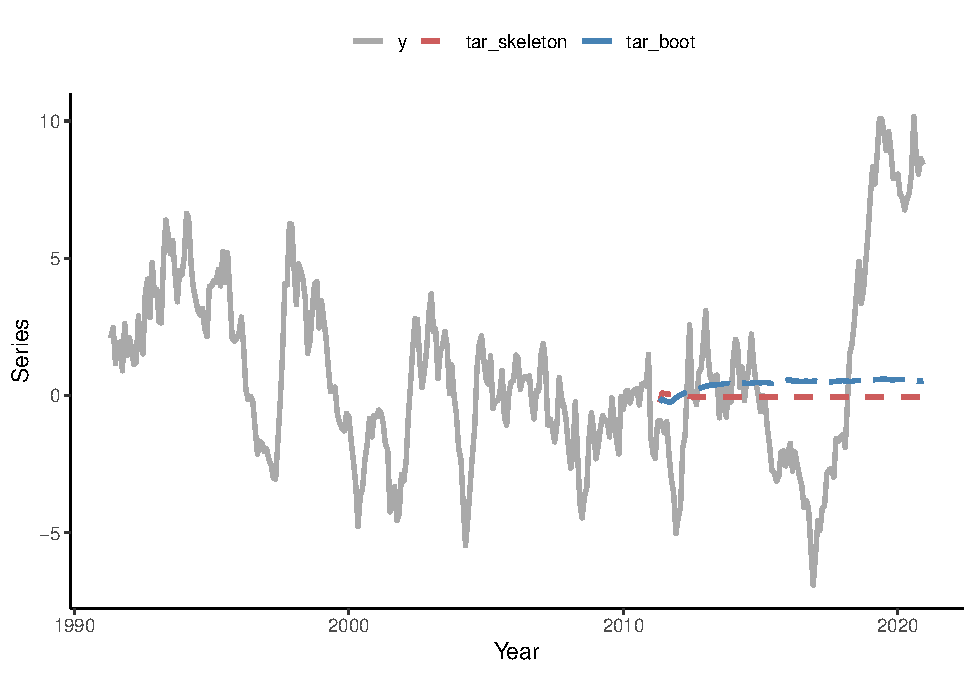
\includegraphics{forecasting_files/figure-latex/unnamed-chunk-88-1.pdf}

\hypertarget{tutorial-8-threshold-autoregression}{%
\chapter*{Tutorial 8: Threshold Autoregression}\label{tutorial-8-threshold-autoregression}}
\addcontentsline{toc}{chapter}{Tutorial 8: Threshold Autoregression}

(this is a evaluation stuff, will need to move back)

In this tutorial, we will generate a time series, we will obtain one-step-ahead forecasts from competing models using a rolling window procedure, and we will perform the Diebold-Mariano type regression-based test for equal predictive ability of the competing models. To run the code, the \texttt{data.table}, \texttt{ggplot2}, \texttt{lmtest}, and \texttt{sandwich} packages need to be installed and loaded.

Let's generate a time series that follow an AR(2) process of the following form:
\[y_t = 0.2+1.1y_{t-1}-0.3y_{t-2}+\varepsilon_t\]
where \(e_{t} \sim N(0,\sigma^2)\).

\begin{Shaded}
\begin{Highlighting}[]
\NormalTok{n }\OtherTok{\textless{}{-}} \DecValTok{240}

\FunctionTok{set.seed}\NormalTok{(}\DecValTok{6}\NormalTok{)}
\NormalTok{e }\OtherTok{\textless{}{-}} \FunctionTok{rnorm}\NormalTok{(n,}\DecValTok{0}\NormalTok{,}\DecValTok{1}\NormalTok{)}

\NormalTok{y }\OtherTok{\textless{}{-}} \FunctionTok{rep}\NormalTok{(}\ConstantTok{NA}\NormalTok{,n)}
\NormalTok{y[}\DecValTok{1}\NormalTok{] }\OtherTok{\textless{}{-}} \FloatTok{0.2}\SpecialCharTok{+}\NormalTok{e[}\DecValTok{1}\NormalTok{]}
\NormalTok{y[}\DecValTok{2}\NormalTok{] }\OtherTok{\textless{}{-}} \FloatTok{0.2+1.1}\SpecialCharTok{*}\NormalTok{y[}\DecValTok{1}\NormalTok{]}\SpecialCharTok{+}\NormalTok{e[}\DecValTok{2}\NormalTok{]}
\ControlFlowTok{for}\NormalTok{(i }\ControlFlowTok{in} \DecValTok{3}\SpecialCharTok{:}\NormalTok{n)\{}
\NormalTok{  y[i] }\OtherTok{\textless{}{-}} \FloatTok{0.2+1.1}\SpecialCharTok{*}\NormalTok{y[i}\DecValTok{{-}1}\NormalTok{]}\SpecialCharTok{{-}}\FloatTok{0.3}\SpecialCharTok{*}\NormalTok{y[i}\DecValTok{{-}2}\NormalTok{]}\SpecialCharTok{+}\NormalTok{e[i]}
\NormalTok{\}}
\end{Highlighting}
\end{Shaded}

Generate a vector of some arbitrary dates (e.g., suppose we deal with the monthly series beginning from January 2000), store these along with \(y\) in a \textbf{data.table}, call it `dt,' and plot the realized time series using \textbf{ggplot} function.

\begin{Shaded}
\begin{Highlighting}[]
\NormalTok{date }\OtherTok{\textless{}{-}} \FunctionTok{seq}\NormalTok{(}\FunctionTok{as.Date}\NormalTok{(}\StringTok{"2000{-}01{-}01"}\NormalTok{),}\AttributeTok{by=}\StringTok{"month"}\NormalTok{,}\AttributeTok{along.with=}\NormalTok{y)}

\NormalTok{dt }\OtherTok{\textless{}{-}} \FunctionTok{data.table}\NormalTok{(date,y)}

\FunctionTok{ggplot}\NormalTok{(dt,}\FunctionTok{aes}\NormalTok{(}\AttributeTok{x=}\NormalTok{date,}\AttributeTok{y=}\NormalTok{y))}\SpecialCharTok{+}
  \FunctionTok{geom\_line}\NormalTok{(}\AttributeTok{size=}\DecValTok{1}\NormalTok{)}\SpecialCharTok{+}
  \FunctionTok{labs}\NormalTok{(}\AttributeTok{x=}\StringTok{"Year"}\NormalTok{,}\AttributeTok{y=}\StringTok{"Series"}\NormalTok{)}\SpecialCharTok{+}
  \FunctionTok{theme\_classic}\NormalTok{()}
\end{Highlighting}
\end{Shaded}

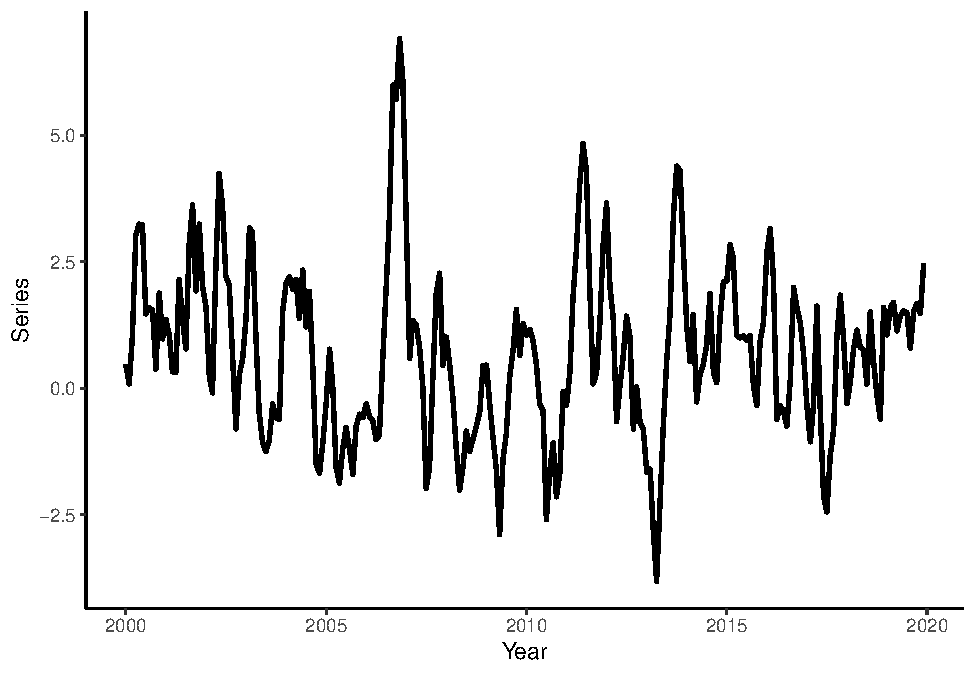
\includegraphics{forecasting_files/figure-latex/unnamed-chunk-91-1.pdf}

Suppose the candidate models are AR(1), AR(2), and AR(3), and that we want to compare forecasts obtained from these models to those from a random walk process. Generate a sequence of one-step-ahead forecasts using the rolling window scheme, where the first rolling window ranges from period 1 to period 180. Calculate the RMSFE measures for the canddidate models.

\begin{Shaded}
\begin{Highlighting}[]
\NormalTok{dt[,}\StringTok{\textasciigrave{}}\AttributeTok{:=}\StringTok{\textasciigrave{}}\NormalTok{(}\AttributeTok{y1=}\FunctionTok{shift}\NormalTok{(y,}\DecValTok{1}\NormalTok{),}\AttributeTok{y2=}\FunctionTok{shift}\NormalTok{(y,}\DecValTok{2}\NormalTok{),}\AttributeTok{y3=}\FunctionTok{shift}\NormalTok{(y,}\DecValTok{3}\NormalTok{))]}

\NormalTok{R }\OtherTok{\textless{}{-}} \DecValTok{180}
\NormalTok{P }\OtherTok{\textless{}{-}} \FunctionTok{nrow}\NormalTok{(dt)}\SpecialCharTok{{-}}\NormalTok{R}

\NormalTok{dt[,}\StringTok{\textasciigrave{}}\AttributeTok{:=}\StringTok{\textasciigrave{}}\NormalTok{(}\AttributeTok{rw=}\FunctionTok{as.numeric}\NormalTok{(}\ConstantTok{NA}\NormalTok{),}\AttributeTok{a1=}\FunctionTok{as.numeric}\NormalTok{(}\ConstantTok{NA}\NormalTok{),}\AttributeTok{a2=}\FunctionTok{as.numeric}\NormalTok{(}\ConstantTok{NA}\NormalTok{),}\AttributeTok{a3=}\FunctionTok{as.numeric}\NormalTok{(}\ConstantTok{NA}\NormalTok{))]}

\ControlFlowTok{for}\NormalTok{(i }\ControlFlowTok{in} \DecValTok{1}\SpecialCharTok{:}\NormalTok{P)\{}
  
\NormalTok{  dt}\SpecialCharTok{$}\NormalTok{rw[R}\SpecialCharTok{+}\NormalTok{i] }\OtherTok{\textless{}{-}}\NormalTok{ dt}\SpecialCharTok{$}\NormalTok{y[R}\SpecialCharTok{+}\NormalTok{i}\DecValTok{{-}1}\NormalTok{]}
  
\NormalTok{  ar1 }\OtherTok{\textless{}{-}} \FunctionTok{lm}\NormalTok{(y}\SpecialCharTok{\textasciitilde{}}\NormalTok{y1,}\AttributeTok{data=}\NormalTok{dt[i}\SpecialCharTok{:}\NormalTok{(R}\SpecialCharTok{+}\NormalTok{i}\DecValTok{{-}1}\NormalTok{)])}
\NormalTok{  ar2 }\OtherTok{\textless{}{-}} \FunctionTok{lm}\NormalTok{(y}\SpecialCharTok{\textasciitilde{}}\NormalTok{y1}\SpecialCharTok{+}\NormalTok{y2,}\AttributeTok{data=}\NormalTok{dt[i}\SpecialCharTok{:}\NormalTok{(R}\SpecialCharTok{+}\NormalTok{i}\DecValTok{{-}1}\NormalTok{)])}
\NormalTok{  ar3 }\OtherTok{\textless{}{-}} \FunctionTok{lm}\NormalTok{(y}\SpecialCharTok{\textasciitilde{}}\NormalTok{y1}\SpecialCharTok{+}\NormalTok{y2}\SpecialCharTok{+}\NormalTok{y3,}\AttributeTok{data=}\NormalTok{dt[i}\SpecialCharTok{:}\NormalTok{(R}\SpecialCharTok{+}\NormalTok{i}\DecValTok{{-}1}\NormalTok{)])}
  
\NormalTok{  dt}\SpecialCharTok{$}\NormalTok{a1[R}\SpecialCharTok{+}\NormalTok{i] }\OtherTok{\textless{}{-}}\NormalTok{ ar1}\SpecialCharTok{$}\NormalTok{coefficients}\SpecialCharTok{\%*\%}\FunctionTok{as.numeric}\NormalTok{(}\FunctionTok{c}\NormalTok{(}\DecValTok{1}\NormalTok{,dt[R}\SpecialCharTok{+}\NormalTok{i,}\FunctionTok{c}\NormalTok{(}\StringTok{"y1"}\NormalTok{)]))}
\NormalTok{  dt}\SpecialCharTok{$}\NormalTok{a2[R}\SpecialCharTok{+}\NormalTok{i] }\OtherTok{\textless{}{-}}\NormalTok{ ar2}\SpecialCharTok{$}\NormalTok{coefficients}\SpecialCharTok{\%*\%}\FunctionTok{as.numeric}\NormalTok{(}\FunctionTok{c}\NormalTok{(}\DecValTok{1}\NormalTok{,dt[R}\SpecialCharTok{+}\NormalTok{i,}\FunctionTok{c}\NormalTok{(}\StringTok{"y1"}\NormalTok{,}\StringTok{"y2"}\NormalTok{)]))}
\NormalTok{  dt}\SpecialCharTok{$}\NormalTok{a3[R}\SpecialCharTok{+}\NormalTok{i] }\OtherTok{\textless{}{-}}\NormalTok{ ar3}\SpecialCharTok{$}\NormalTok{coefficients}\SpecialCharTok{\%*\%}\FunctionTok{as.numeric}\NormalTok{(}\FunctionTok{c}\NormalTok{(}\DecValTok{1}\NormalTok{,dt[R}\SpecialCharTok{+}\NormalTok{i,}\FunctionTok{c}\NormalTok{(}\StringTok{"y1"}\NormalTok{,}\StringTok{"y2"}\NormalTok{,}\StringTok{"y3"}\NormalTok{)]))}
  
\NormalTok{\}}

\NormalTok{dt}\SpecialCharTok{$}\NormalTok{rw\_e }\OtherTok{\textless{}{-}}\NormalTok{ dt}\SpecialCharTok{$}\NormalTok{y}\SpecialCharTok{{-}}\NormalTok{dt}\SpecialCharTok{$}\NormalTok{rw}
\NormalTok{dt}\SpecialCharTok{$}\NormalTok{a1\_e }\OtherTok{\textless{}{-}}\NormalTok{ dt}\SpecialCharTok{$}\NormalTok{y}\SpecialCharTok{{-}}\NormalTok{dt}\SpecialCharTok{$}\NormalTok{a1}
\NormalTok{dt}\SpecialCharTok{$}\NormalTok{a2\_e }\OtherTok{\textless{}{-}}\NormalTok{ dt}\SpecialCharTok{$}\NormalTok{y}\SpecialCharTok{{-}}\NormalTok{dt}\SpecialCharTok{$}\NormalTok{a2}
\NormalTok{dt}\SpecialCharTok{$}\NormalTok{a3\_e }\OtherTok{\textless{}{-}}\NormalTok{ dt}\SpecialCharTok{$}\NormalTok{y}\SpecialCharTok{{-}}\NormalTok{dt}\SpecialCharTok{$}\NormalTok{a3}

\CommentTok{\# RMSFEs}
\FunctionTok{sqrt}\NormalTok{(}\FunctionTok{mean}\NormalTok{(dt}\SpecialCharTok{$}\NormalTok{rw\_e}\SpecialCharTok{\^{}}\DecValTok{2}\NormalTok{,}\AttributeTok{na.rm=}\NormalTok{T))}
\end{Highlighting}
\end{Shaded}

\begin{verbatim}
## [1] 0.9653331
\end{verbatim}

\begin{Shaded}
\begin{Highlighting}[]
\FunctionTok{sqrt}\NormalTok{(}\FunctionTok{mean}\NormalTok{(dt}\SpecialCharTok{$}\NormalTok{a1\_e}\SpecialCharTok{\^{}}\DecValTok{2}\NormalTok{,}\AttributeTok{na.rm=}\NormalTok{T))}
\end{Highlighting}
\end{Shaded}

\begin{verbatim}
## [1] 0.9053279
\end{verbatim}

\begin{Shaded}
\begin{Highlighting}[]
\FunctionTok{sqrt}\NormalTok{(}\FunctionTok{mean}\NormalTok{(dt}\SpecialCharTok{$}\NormalTok{a2\_e}\SpecialCharTok{\^{}}\DecValTok{2}\NormalTok{,}\AttributeTok{na.rm=}\NormalTok{T))}
\end{Highlighting}
\end{Shaded}

\begin{verbatim}
## [1] 0.8842908
\end{verbatim}

\begin{Shaded}
\begin{Highlighting}[]
\FunctionTok{sqrt}\NormalTok{(}\FunctionTok{mean}\NormalTok{(dt}\SpecialCharTok{$}\NormalTok{a3\_e}\SpecialCharTok{\^{}}\DecValTok{2}\NormalTok{,}\AttributeTok{na.rm=}\NormalTok{T))}
\end{Highlighting}
\end{Shaded}

\begin{verbatim}
## [1] 0.8877883
\end{verbatim}

Do the autoregressive models generate `statistically significantly' more accurate forecasts than the random walk model? We will answer this question by performing the regression-based Diebold-Mariano tests. First we will generate the loss differentials; then we will run three separate regressions to assess predictive accuracy of AR(1), AR(2), and AR(3) relative to the random walk; and finally we will base our decision on the heteroskedasticity and autocorrelation consistent standard errors.

\begin{Shaded}
\begin{Highlighting}[]
\NormalTok{dt}\SpecialCharTok{$}\NormalTok{ld1 }\OtherTok{\textless{}{-}}\NormalTok{ dt}\SpecialCharTok{$}\NormalTok{rw\_e}\SpecialCharTok{\^{}}\DecValTok{2}\SpecialCharTok{{-}}\NormalTok{dt}\SpecialCharTok{$}\NormalTok{a1\_e}\SpecialCharTok{\^{}}\DecValTok{2}
\NormalTok{dt}\SpecialCharTok{$}\NormalTok{ld2 }\OtherTok{\textless{}{-}}\NormalTok{ dt}\SpecialCharTok{$}\NormalTok{rw\_e}\SpecialCharTok{\^{}}\DecValTok{2}\SpecialCharTok{{-}}\NormalTok{dt}\SpecialCharTok{$}\NormalTok{a2\_e}\SpecialCharTok{\^{}}\DecValTok{2}
\NormalTok{dt}\SpecialCharTok{$}\NormalTok{ld3 }\OtherTok{\textless{}{-}}\NormalTok{ dt}\SpecialCharTok{$}\NormalTok{rw\_e}\SpecialCharTok{\^{}}\DecValTok{2}\SpecialCharTok{{-}}\NormalTok{dt}\SpecialCharTok{$}\NormalTok{a3\_e}\SpecialCharTok{\^{}}\DecValTok{2}

\NormalTok{reg.ld1 }\OtherTok{\textless{}{-}} \FunctionTok{lm}\NormalTok{(ld1}\SpecialCharTok{\textasciitilde{}}\DecValTok{1}\NormalTok{,}\AttributeTok{data=}\NormalTok{dt)}
\NormalTok{reg.ld2 }\OtherTok{\textless{}{-}} \FunctionTok{lm}\NormalTok{(ld2}\SpecialCharTok{\textasciitilde{}}\DecValTok{1}\NormalTok{,}\AttributeTok{data=}\NormalTok{dt)}
\NormalTok{reg.ld3 }\OtherTok{\textless{}{-}} \FunctionTok{lm}\NormalTok{(ld3}\SpecialCharTok{\textasciitilde{}}\DecValTok{1}\NormalTok{,}\AttributeTok{data=}\NormalTok{dt)}

\FunctionTok{coeftest}\NormalTok{(reg.ld1,}\AttributeTok{vcov.=}\FunctionTok{vcovHAC}\NormalTok{(reg.ld1))}
\end{Highlighting}
\end{Shaded}

\begin{verbatim}
## 
## t test of coefficients:
## 
##             Estimate Std. Error t value Pr(>|t|)  
## (Intercept) 0.112249   0.047525  2.3619   0.0215 *
## ---
## Signif. codes:  0 '***' 0.001 '**' 0.01 '*' 0.05 '.' 0.1 ' ' 1
\end{verbatim}

\begin{Shaded}
\begin{Highlighting}[]
\FunctionTok{coeftest}\NormalTok{(reg.ld2,}\AttributeTok{vcov.=}\FunctionTok{vcovHAC}\NormalTok{(reg.ld2))}
\end{Highlighting}
\end{Shaded}

\begin{verbatim}
## 
## t test of coefficients:
## 
##             Estimate Std. Error t value Pr(>|t|)  
## (Intercept) 0.149898   0.083086  1.8041  0.07632 .
## ---
## Signif. codes:  0 '***' 0.001 '**' 0.01 '*' 0.05 '.' 0.1 ' ' 1
\end{verbatim}

\begin{Shaded}
\begin{Highlighting}[]
\FunctionTok{coeftest}\NormalTok{(reg.ld3,}\AttributeTok{vcov.=}\FunctionTok{vcovHAC}\NormalTok{(reg.ld3))}
\end{Highlighting}
\end{Shaded}

\begin{verbatim}
## 
## t test of coefficients:
## 
##             Estimate Std. Error t value Pr(>|t|)  
## (Intercept) 0.143700   0.081309  1.7673  0.08235 .
## ---
## Signif. codes:  0 '***' 0.001 '**' 0.01 '*' 0.05 '.' 0.1 ' ' 1
\end{verbatim}

\hypertarget{tutorial-9-forecast-evaluation}{%
\chapter*{Tutorial 9: Forecast Evaluation}\label{tutorial-9-forecast-evaluation}}
\addcontentsline{toc}{chapter}{Tutorial 9: Forecast Evaluation}

(this is a combination stuff, will need to move back)

In this tutorial, we will generate a time series, we will obtain one-step-ahead forecasts from a set of models using a rolling window procedure, we will combine these forecasts and assess the accuracy of the combined forecast. To run the code, the \texttt{data.table}, \texttt{ggplot2}, \texttt{lmtest}, and \texttt{sandwich} packages need to be installed and loaded.

Let's generate a time series that follow an AR(2) process with the quadratic trend component as follows:
\[y_t = 0.03t-0.0001t^2+0.6y_{t-1}+0.2y_{t-2}+\varepsilon_t\]
where \(e_{t} \sim N(0,\sigma^2)\).

\begin{Shaded}
\begin{Highlighting}[]
\NormalTok{n }\OtherTok{\textless{}{-}} \DecValTok{240}

\FunctionTok{set.seed}\NormalTok{(}\DecValTok{4}\NormalTok{)}
\NormalTok{e }\OtherTok{\textless{}{-}} \FunctionTok{rnorm}\NormalTok{(n,}\DecValTok{0}\NormalTok{,}\DecValTok{1}\NormalTok{)}

\NormalTok{y }\OtherTok{\textless{}{-}} \FunctionTok{rep}\NormalTok{(}\ConstantTok{NA}\NormalTok{,n)}
\NormalTok{y[}\DecValTok{1}\NormalTok{] }\OtherTok{\textless{}{-}} \FloatTok{0.03}\SpecialCharTok{*}\DecValTok{1}\FloatTok{{-}0.0001}\SpecialCharTok{*}\NormalTok{(}\DecValTok{1}\SpecialCharTok{\^{}}\DecValTok{2}\NormalTok{)}\SpecialCharTok{+}\NormalTok{e[}\DecValTok{1}\NormalTok{]}
\NormalTok{y[}\DecValTok{2}\NormalTok{] }\OtherTok{\textless{}{-}} \FloatTok{0.03}\SpecialCharTok{*}\DecValTok{2}\FloatTok{{-}0.0001}\SpecialCharTok{*}\NormalTok{(}\DecValTok{2}\SpecialCharTok{\^{}}\DecValTok{2}\NormalTok{)}\SpecialCharTok{+}\FloatTok{0.6}\SpecialCharTok{*}\NormalTok{y[}\DecValTok{1}\NormalTok{]}\SpecialCharTok{+}\NormalTok{e[}\DecValTok{2}\NormalTok{]}
\ControlFlowTok{for}\NormalTok{(i }\ControlFlowTok{in} \DecValTok{3}\SpecialCharTok{:}\NormalTok{n)\{}
\NormalTok{  y[i] }\OtherTok{\textless{}{-}} \FloatTok{0.03}\SpecialCharTok{*}\NormalTok{i}\FloatTok{{-}0.0001}\SpecialCharTok{*}\NormalTok{(i}\SpecialCharTok{\^{}}\DecValTok{2}\NormalTok{)}\SpecialCharTok{+}\FloatTok{0.6}\SpecialCharTok{*}\NormalTok{y[i}\DecValTok{{-}1}\NormalTok{]}\SpecialCharTok{+}\FloatTok{0.2}\SpecialCharTok{*}\NormalTok{y[i}\DecValTok{{-}2}\NormalTok{]}\SpecialCharTok{+}\NormalTok{e[i]}
\NormalTok{\}}
\end{Highlighting}
\end{Shaded}

Generate a vector of some arbitrary dates (e.g., suppose we deal with the monthly series beginning from January 2000), store these along with \(y\) in a \textbf{data.table}, call it `dt,' and plot the realized time series using \textbf{ggplot} function.

\begin{Shaded}
\begin{Highlighting}[]
\NormalTok{date }\OtherTok{\textless{}{-}} \FunctionTok{seq}\NormalTok{(}\FunctionTok{as.Date}\NormalTok{(}\StringTok{"2000{-}01{-}01"}\NormalTok{),}\AttributeTok{by=}\StringTok{"month"}\NormalTok{,}\AttributeTok{along.with=}\NormalTok{y)}

\NormalTok{dt }\OtherTok{\textless{}{-}} \FunctionTok{data.table}\NormalTok{(date,y)}

\FunctionTok{ggplot}\NormalTok{(dt,}\FunctionTok{aes}\NormalTok{(}\AttributeTok{x=}\NormalTok{date,}\AttributeTok{y=}\NormalTok{y))}\SpecialCharTok{+}
  \FunctionTok{geom\_line}\NormalTok{(}\AttributeTok{size=}\DecValTok{1}\NormalTok{)}\SpecialCharTok{+}
  \FunctionTok{labs}\NormalTok{(}\AttributeTok{x=}\StringTok{"Year"}\NormalTok{,}\AttributeTok{y=}\StringTok{"Series"}\NormalTok{)}\SpecialCharTok{+}
  \FunctionTok{theme\_classic}\NormalTok{()}
\end{Highlighting}
\end{Shaded}

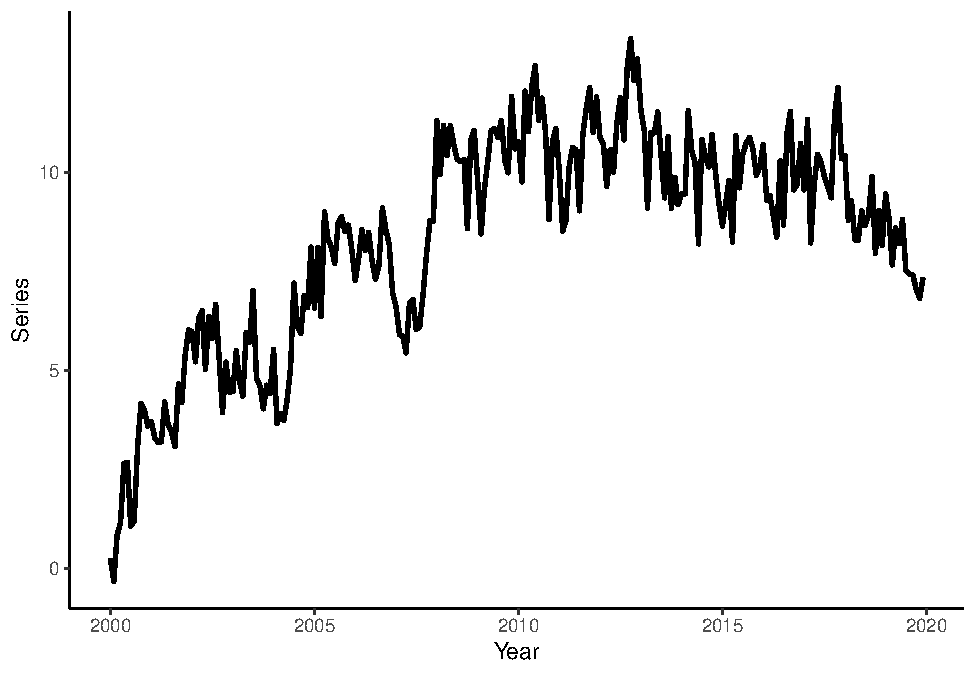
\includegraphics{forecasting_files/figure-latex/unnamed-chunk-96-1.pdf}

Suppose the candidate models are AR(1), AR(2), and a linear trend model, and that we want to compare forecasts obtained from these models to those from a random walk process. Generate a sequence of one-step-ahead forecasts using the rolling window scheme, where the first rolling window ranges from period 1 to period 180.

\begin{Shaded}
\begin{Highlighting}[]
\NormalTok{dt[,}\StringTok{\textasciigrave{}}\AttributeTok{:=}\StringTok{\textasciigrave{}}\NormalTok{(}\AttributeTok{y1=}\FunctionTok{shift}\NormalTok{(y,}\DecValTok{1}\NormalTok{),}\AttributeTok{y2=}\FunctionTok{shift}\NormalTok{(y,}\DecValTok{2}\NormalTok{),}\AttributeTok{y3=}\FunctionTok{shift}\NormalTok{(y,}\DecValTok{3}\NormalTok{),}\AttributeTok{trend=}\FunctionTok{c}\NormalTok{(}\DecValTok{1}\SpecialCharTok{:}\FunctionTok{nrow}\NormalTok{(dt)))]}

\NormalTok{R }\OtherTok{\textless{}{-}} \DecValTok{180}
\NormalTok{P }\OtherTok{\textless{}{-}} \FunctionTok{nrow}\NormalTok{(dt)}\SpecialCharTok{{-}}\NormalTok{R}

\NormalTok{dt[,}\StringTok{\textasciigrave{}}\AttributeTok{:=}\StringTok{\textasciigrave{}}\NormalTok{(}\AttributeTok{rw=}\FunctionTok{as.numeric}\NormalTok{(}\ConstantTok{NA}\NormalTok{),}\AttributeTok{a1=}\FunctionTok{as.numeric}\NormalTok{(}\ConstantTok{NA}\NormalTok{),}\AttributeTok{a2=}\FunctionTok{as.numeric}\NormalTok{(}\ConstantTok{NA}\NormalTok{),}\AttributeTok{tr=}\FunctionTok{as.numeric}\NormalTok{(}\ConstantTok{NA}\NormalTok{))]}

\ControlFlowTok{for}\NormalTok{(i }\ControlFlowTok{in} \DecValTok{1}\SpecialCharTok{:}\NormalTok{P)\{}
  
\NormalTok{  dt}\SpecialCharTok{$}\NormalTok{rw[R}\SpecialCharTok{+}\NormalTok{i] }\OtherTok{\textless{}{-}}\NormalTok{ dt}\SpecialCharTok{$}\NormalTok{y[R}\SpecialCharTok{+}\NormalTok{i}\DecValTok{{-}1}\NormalTok{]}
  
\NormalTok{  a1 }\OtherTok{\textless{}{-}} \FunctionTok{lm}\NormalTok{(y}\SpecialCharTok{\textasciitilde{}}\NormalTok{y1,}\AttributeTok{data=}\NormalTok{dt[i}\SpecialCharTok{:}\NormalTok{(R}\SpecialCharTok{+}\NormalTok{i}\DecValTok{{-}1}\NormalTok{)])}
\NormalTok{  a2 }\OtherTok{\textless{}{-}} \FunctionTok{lm}\NormalTok{(y}\SpecialCharTok{\textasciitilde{}}\NormalTok{y1}\SpecialCharTok{+}\NormalTok{y2,}\AttributeTok{data=}\NormalTok{dt[i}\SpecialCharTok{:}\NormalTok{(R}\SpecialCharTok{+}\NormalTok{i}\DecValTok{{-}1}\NormalTok{)])}
\NormalTok{  tr }\OtherTok{\textless{}{-}} \FunctionTok{lm}\NormalTok{(y}\SpecialCharTok{\textasciitilde{}}\NormalTok{y1}\SpecialCharTok{+}\NormalTok{y2}\SpecialCharTok{+}\NormalTok{trend,}\AttributeTok{data=}\NormalTok{dt[i}\SpecialCharTok{:}\NormalTok{(R}\SpecialCharTok{+}\NormalTok{i}\DecValTok{{-}1}\NormalTok{)])}
  
\NormalTok{  dt}\SpecialCharTok{$}\NormalTok{a1[R}\SpecialCharTok{+}\NormalTok{i] }\OtherTok{\textless{}{-}}\NormalTok{ a1}\SpecialCharTok{$}\NormalTok{coefficients}\SpecialCharTok{\%*\%}\FunctionTok{as.numeric}\NormalTok{(}\FunctionTok{c}\NormalTok{(}\DecValTok{1}\NormalTok{,dt[R}\SpecialCharTok{+}\NormalTok{i,}\FunctionTok{c}\NormalTok{(}\StringTok{"y1"}\NormalTok{)]))}
\NormalTok{  dt}\SpecialCharTok{$}\NormalTok{a2[R}\SpecialCharTok{+}\NormalTok{i] }\OtherTok{\textless{}{-}}\NormalTok{ a2}\SpecialCharTok{$}\NormalTok{coefficients}\SpecialCharTok{\%*\%}\FunctionTok{as.numeric}\NormalTok{(}\FunctionTok{c}\NormalTok{(}\DecValTok{1}\NormalTok{,dt[R}\SpecialCharTok{+}\NormalTok{i,}\FunctionTok{c}\NormalTok{(}\StringTok{"y1"}\NormalTok{,}\StringTok{"y2"}\NormalTok{)]))}
\NormalTok{  dt}\SpecialCharTok{$}\NormalTok{tr[R}\SpecialCharTok{+}\NormalTok{i] }\OtherTok{\textless{}{-}}\NormalTok{ tr}\SpecialCharTok{$}\NormalTok{coefficients}\SpecialCharTok{\%*\%}\FunctionTok{as.numeric}\NormalTok{(}\FunctionTok{c}\NormalTok{(}\DecValTok{1}\NormalTok{,dt[R}\SpecialCharTok{+}\NormalTok{i,}\FunctionTok{c}\NormalTok{(}\StringTok{"y1"}\NormalTok{,}\StringTok{"y2"}\NormalTok{,}\StringTok{"trend"}\NormalTok{)]))}
  
\NormalTok{\}}
\end{Highlighting}
\end{Shaded}

Does either of the considered models `sttaistically significantly' outperform the random walk?

\begin{Shaded}
\begin{Highlighting}[]
\NormalTok{dt}\SpecialCharTok{$}\NormalTok{rw\_e }\OtherTok{\textless{}{-}}\NormalTok{ dt}\SpecialCharTok{$}\NormalTok{y}\SpecialCharTok{{-}}\NormalTok{dt}\SpecialCharTok{$}\NormalTok{rw}
\NormalTok{dt}\SpecialCharTok{$}\NormalTok{a1\_e }\OtherTok{\textless{}{-}}\NormalTok{ dt}\SpecialCharTok{$}\NormalTok{y}\SpecialCharTok{{-}}\NormalTok{dt}\SpecialCharTok{$}\NormalTok{a1}
\NormalTok{dt}\SpecialCharTok{$}\NormalTok{a2\_e }\OtherTok{\textless{}{-}}\NormalTok{ dt}\SpecialCharTok{$}\NormalTok{y}\SpecialCharTok{{-}}\NormalTok{dt}\SpecialCharTok{$}\NormalTok{a2}
\NormalTok{dt}\SpecialCharTok{$}\NormalTok{tr\_e }\OtherTok{\textless{}{-}}\NormalTok{ dt}\SpecialCharTok{$}\NormalTok{y}\SpecialCharTok{{-}}\NormalTok{dt}\SpecialCharTok{$}\NormalTok{tr}

\NormalTok{dt}\SpecialCharTok{$}\NormalTok{ld1 }\OtherTok{\textless{}{-}}\NormalTok{ dt}\SpecialCharTok{$}\NormalTok{rw\_e}\SpecialCharTok{\^{}}\DecValTok{2}\SpecialCharTok{{-}}\NormalTok{dt}\SpecialCharTok{$}\NormalTok{a1\_e}\SpecialCharTok{\^{}}\DecValTok{2}
\NormalTok{dt}\SpecialCharTok{$}\NormalTok{ld2 }\OtherTok{\textless{}{-}}\NormalTok{ dt}\SpecialCharTok{$}\NormalTok{rw\_e}\SpecialCharTok{\^{}}\DecValTok{2}\SpecialCharTok{{-}}\NormalTok{dt}\SpecialCharTok{$}\NormalTok{a2\_e}\SpecialCharTok{\^{}}\DecValTok{2}
\NormalTok{dt}\SpecialCharTok{$}\NormalTok{ldt }\OtherTok{\textless{}{-}}\NormalTok{ dt}\SpecialCharTok{$}\NormalTok{rw\_e}\SpecialCharTok{\^{}}\DecValTok{2}\SpecialCharTok{{-}}\NormalTok{dt}\SpecialCharTok{$}\NormalTok{tr\_e}\SpecialCharTok{\^{}}\DecValTok{2}

\NormalTok{reg.ld1 }\OtherTok{\textless{}{-}} \FunctionTok{lm}\NormalTok{(ld1}\SpecialCharTok{\textasciitilde{}}\DecValTok{1}\NormalTok{,}\AttributeTok{data=}\NormalTok{dt)}
\NormalTok{reg.ld2 }\OtherTok{\textless{}{-}} \FunctionTok{lm}\NormalTok{(ld2}\SpecialCharTok{\textasciitilde{}}\DecValTok{1}\NormalTok{,}\AttributeTok{data=}\NormalTok{dt)}
\NormalTok{reg.ldt }\OtherTok{\textless{}{-}} \FunctionTok{lm}\NormalTok{(ldt}\SpecialCharTok{\textasciitilde{}}\DecValTok{1}\NormalTok{,}\AttributeTok{data=}\NormalTok{dt)}

\FunctionTok{coeftest}\NormalTok{(reg.ld1,}\AttributeTok{vcov.=}\FunctionTok{vcovHAC}\NormalTok{(reg.ld1))}
\end{Highlighting}
\end{Shaded}

\begin{verbatim}
## 
## t test of coefficients:
## 
##             Estimate Std. Error t value Pr(>|t|)  
## (Intercept) 0.081204   0.048040  1.6903  0.09624 .
## ---
## Signif. codes:  0 '***' 0.001 '**' 0.01 '*' 0.05 '.' 0.1 ' ' 1
\end{verbatim}

\begin{Shaded}
\begin{Highlighting}[]
\FunctionTok{coeftest}\NormalTok{(reg.ld2,}\AttributeTok{vcov.=}\FunctionTok{vcovHAC}\NormalTok{(reg.ld2))}
\end{Highlighting}
\end{Shaded}

\begin{verbatim}
## 
## t test of coefficients:
## 
##             Estimate Std. Error t value Pr(>|t|)  
## (Intercept)  0.32634    0.14912  2.1883  0.03262 *
## ---
## Signif. codes:  0 '***' 0.001 '**' 0.01 '*' 0.05 '.' 0.1 ' ' 1
\end{verbatim}

\begin{Shaded}
\begin{Highlighting}[]
\FunctionTok{coeftest}\NormalTok{(reg.ldt,}\AttributeTok{vcov.=}\FunctionTok{vcovHAC}\NormalTok{(reg.ldt))}
\end{Highlighting}
\end{Shaded}

\begin{verbatim}
## 
## t test of coefficients:
## 
##             Estimate Std. Error t value Pr(>|t|)
## (Intercept)  0.24461    0.14943  1.6369    0.107
\end{verbatim}

All of the models do, on average, generate more accurate forecasts than random walk. The AR(2) generates statistically significantly more accurate forecasts, based on Diebold-Mariano test applied on quadratic loss function.

Might each model contain some useful information for improving forecast accuracy? Let's combine the forecasts from the AR(1) and the linear trend model using equal weights scheme and assess the combined forecast.

\begin{Shaded}
\begin{Highlighting}[]
\NormalTok{dt}\SpecialCharTok{$}\NormalTok{t1 }\OtherTok{\textless{}{-}}\NormalTok{ dt}\SpecialCharTok{$}\NormalTok{a1}\SpecialCharTok{*}\NormalTok{.}\DecValTok{5}\SpecialCharTok{+}\NormalTok{dt}\SpecialCharTok{$}\NormalTok{tr}\SpecialCharTok{*}\NormalTok{.}\DecValTok{5}
\NormalTok{dt}\SpecialCharTok{$}\NormalTok{t1\_e }\OtherTok{\textless{}{-}}\NormalTok{ dt}\SpecialCharTok{$}\NormalTok{y}\SpecialCharTok{{-}}\NormalTok{dt}\SpecialCharTok{$}\NormalTok{t1}

\NormalTok{dt}\SpecialCharTok{$}\NormalTok{ldt1 }\OtherTok{\textless{}{-}}\NormalTok{ dt}\SpecialCharTok{$}\NormalTok{rw\_e}\SpecialCharTok{\^{}}\DecValTok{2}\SpecialCharTok{{-}}\NormalTok{dt}\SpecialCharTok{$}\NormalTok{t1\_e}\SpecialCharTok{\^{}}\DecValTok{2}

\NormalTok{reg.ldt1 }\OtherTok{\textless{}{-}} \FunctionTok{lm}\NormalTok{(ldt1}\SpecialCharTok{\textasciitilde{}}\DecValTok{1}\NormalTok{,}\AttributeTok{data=}\NormalTok{dt)}

\FunctionTok{coeftest}\NormalTok{(reg.ldt1,}\AttributeTok{vcov.=}\FunctionTok{vcovHAC}\NormalTok{(reg.ldt1))}
\end{Highlighting}
\end{Shaded}

\begin{verbatim}
## 
## t test of coefficients:
## 
##             Estimate Std. Error t value Pr(>|t|)  
## (Intercept) 0.232926   0.098544  2.3637  0.02141 *
## ---
## Signif. codes:  0 '***' 0.001 '**' 0.01 '*' 0.05 '.' 0.1 ' ' 1
\end{verbatim}

\hypertarget{tutorial-10-forecast-combination}{%
\chapter*{Tutorial 10: Forecast Combination}\label{tutorial-10-forecast-combination}}
\addcontentsline{toc}{chapter}{Tutorial 10: Forecast Combination}

(this is a direct/iterated stuff, will need to move forward)

In this tutorial, we will generate a time series, we will obtain multi-step-ahead forecasts using direct and iterated methods from autoregressive models using a rolling window procedure, and we will assess the accuracy of the forecast. We will then turn to interval forecasts, and we will assess their coverage accuracy. To run the code, the \texttt{data.table}, \texttt{ggplot2}, \texttt{lmtest}, and \texttt{sandwich} packages need to be installed and loaded.

Let's generate a time series that follow an AR(2) process as follows:
\[y_t = 0.01t+0.6y_{t-1}+0.2y_{t-2}+\varepsilon_t\]
where \(e_{t} \sim N(0,1)\).

\begin{Shaded}
\begin{Highlighting}[]
\NormalTok{n }\OtherTok{\textless{}{-}} \DecValTok{240}

\FunctionTok{set.seed}\NormalTok{(}\DecValTok{9}\NormalTok{)}
\NormalTok{e }\OtherTok{\textless{}{-}} \FunctionTok{rnorm}\NormalTok{(n,}\DecValTok{0}\NormalTok{,}\DecValTok{1}\NormalTok{)}

\NormalTok{y }\OtherTok{\textless{}{-}} \FunctionTok{rep}\NormalTok{(}\ConstantTok{NA}\NormalTok{,n)}
\NormalTok{y[}\DecValTok{1}\NormalTok{] }\OtherTok{\textless{}{-}} \FloatTok{0.01}\SpecialCharTok{+}\NormalTok{e[}\DecValTok{1}\NormalTok{]}
\NormalTok{y[}\DecValTok{2}\NormalTok{] }\OtherTok{\textless{}{-}} \FloatTok{0.02+0.6}\SpecialCharTok{*}\NormalTok{y[}\DecValTok{1}\NormalTok{]}\SpecialCharTok{+}\NormalTok{e[}\DecValTok{2}\NormalTok{]}
\ControlFlowTok{for}\NormalTok{(i }\ControlFlowTok{in} \DecValTok{3}\SpecialCharTok{:}\NormalTok{n)\{}
\NormalTok{  y[i] }\OtherTok{\textless{}{-}} \FloatTok{0.01}\SpecialCharTok{*}\NormalTok{i}\FloatTok{+0.6}\SpecialCharTok{*}\NormalTok{y[i}\DecValTok{{-}1}\NormalTok{]}\SpecialCharTok{+}\FloatTok{0.2}\SpecialCharTok{*}\NormalTok{y[i}\DecValTok{{-}2}\NormalTok{]}\SpecialCharTok{+}\NormalTok{e[i]}
\NormalTok{\}}
\end{Highlighting}
\end{Shaded}

Generate a vector of arbitrary dates (e.g., the monthly series beginning from January 2000), store these along with \(y\) in a \textbf{data.table}, call it `dt,' and plot the realized time series using the \textbf{ggplot} function.

\begin{Shaded}
\begin{Highlighting}[]
\NormalTok{date }\OtherTok{\textless{}{-}} \FunctionTok{seq}\NormalTok{(}\FunctionTok{as.Date}\NormalTok{(}\StringTok{"2000{-}01{-}01"}\NormalTok{),}\AttributeTok{by=}\StringTok{"month"}\NormalTok{,}\AttributeTok{along.with=}\NormalTok{y)}

\NormalTok{dt }\OtherTok{\textless{}{-}} \FunctionTok{data.table}\NormalTok{(date,y)}

\FunctionTok{ggplot}\NormalTok{(dt,}\FunctionTok{aes}\NormalTok{(}\AttributeTok{x=}\NormalTok{date,}\AttributeTok{y=}\NormalTok{y))}\SpecialCharTok{+}
  \FunctionTok{geom\_line}\NormalTok{(}\AttributeTok{size=}\DecValTok{1}\NormalTok{)}\SpecialCharTok{+}
  \FunctionTok{labs}\NormalTok{(}\AttributeTok{x=}\StringTok{"Year"}\NormalTok{,}\AttributeTok{y=}\StringTok{"Series"}\NormalTok{)}\SpecialCharTok{+}
  \FunctionTok{theme\_classic}\NormalTok{()}
\end{Highlighting}
\end{Shaded}

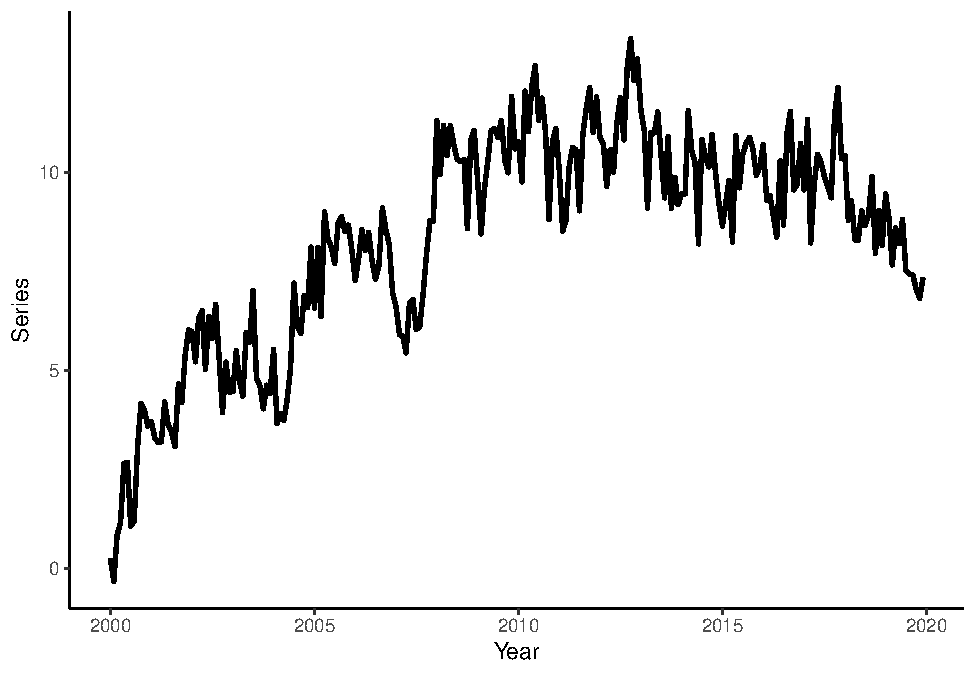
\includegraphics{forecasting_files/figure-latex/unnamed-chunk-102-1.pdf}

Suppose we believe the series follow either the AR(1) or the AR(2) process, and that we want to compare iterated multi-step forecasts obtained from these models to direct multi-step forecasts. In what follows, we will generate twelve-step-ahead point forecasts from these two methods for the considered two models using the rolling window scheme, where the first rolling window ranges from period 1 to period 180. In obtaining the iterated multi-step forecasts, for each rolling window, we will generate a sequence of one-to-twelve-step-ahead forecasts, but only retain the twelve-step-ahead forecasts.

\begin{Shaded}
\begin{Highlighting}[]
\NormalTok{h }\OtherTok{\textless{}{-}} \DecValTok{12}

\NormalTok{dt }\OtherTok{\textless{}{-}}\NormalTok{ dt[,.(date,y,}\AttributeTok{y1=}\FunctionTok{shift}\NormalTok{(y,}\DecValTok{1}\NormalTok{),}\AttributeTok{y2=}\FunctionTok{shift}\NormalTok{(y,}\DecValTok{2}\NormalTok{),}\AttributeTok{y12=}\FunctionTok{shift}\NormalTok{(y,h),}\AttributeTok{y13=}\FunctionTok{shift}\NormalTok{(y,h}\SpecialCharTok{+}\DecValTok{1}\NormalTok{))]}
\NormalTok{dt }\OtherTok{\textless{}{-}}\NormalTok{ dt[}\FunctionTok{complete.cases}\NormalTok{(dt)]}

\NormalTok{dt[,}\StringTok{\textasciigrave{}}\AttributeTok{:=}\StringTok{\textasciigrave{}}\NormalTok{(}\AttributeTok{a1i=}\FunctionTok{as.numeric}\NormalTok{(}\ConstantTok{NA}\NormalTok{),}\AttributeTok{a1d=}\FunctionTok{as.numeric}\NormalTok{(}\ConstantTok{NA}\NormalTok{),}\AttributeTok{a2i=}\FunctionTok{as.numeric}\NormalTok{(}\ConstantTok{NA}\NormalTok{),}\AttributeTok{a2d=}\FunctionTok{as.numeric}\NormalTok{(}\ConstantTok{NA}\NormalTok{))]}

\NormalTok{R }\OtherTok{\textless{}{-}} \DecValTok{180}
\NormalTok{P }\OtherTok{\textless{}{-}} \FunctionTok{nrow}\NormalTok{(dt)}\SpecialCharTok{{-}}\NormalTok{R}\SpecialCharTok{{-}}\NormalTok{h}\SpecialCharTok{+}\DecValTok{1}

\ControlFlowTok{for}\NormalTok{(i }\ControlFlowTok{in} \DecValTok{1}\SpecialCharTok{:}\NormalTok{P)\{}
  
  \DocumentationTok{\#\#\# iterated multi{-}step method}
\NormalTok{  a1i }\OtherTok{\textless{}{-}} \FunctionTok{lm}\NormalTok{(y}\SpecialCharTok{\textasciitilde{}}\NormalTok{y1,}\AttributeTok{data=}\NormalTok{dt[i}\SpecialCharTok{:}\NormalTok{(R}\SpecialCharTok{+}\NormalTok{i}\DecValTok{{-}1}\NormalTok{)])}
\NormalTok{  a2i }\OtherTok{\textless{}{-}} \FunctionTok{lm}\NormalTok{(y}\SpecialCharTok{\textasciitilde{}}\NormalTok{y1}\SpecialCharTok{+}\NormalTok{y2,}\AttributeTok{data=}\NormalTok{dt[i}\SpecialCharTok{:}\NormalTok{(R}\SpecialCharTok{+}\NormalTok{i}\DecValTok{{-}1}\NormalTok{)])}
  
\NormalTok{  iter\_dt }\OtherTok{\textless{}{-}} \FunctionTok{data.table}\NormalTok{(}\AttributeTok{hor=}\DecValTok{1}\SpecialCharTok{:}\NormalTok{h,}\AttributeTok{a1=}\FunctionTok{as.numeric}\NormalTok{(}\ConstantTok{NA}\NormalTok{),}\AttributeTok{a2=}\FunctionTok{as.numeric}\NormalTok{(}\ConstantTok{NA}\NormalTok{))}
  
  \DocumentationTok{\#\# AR(1)}
\NormalTok{  iter\_dt}\SpecialCharTok{$}\NormalTok{a1[}\DecValTok{1}\NormalTok{] }\OtherTok{\textless{}{-}}\NormalTok{ a1i}\SpecialCharTok{$}\NormalTok{coefficients[}\DecValTok{1}\NormalTok{]}\SpecialCharTok{+}\NormalTok{a1i}\SpecialCharTok{$}\NormalTok{coefficients[}\DecValTok{2}\NormalTok{]}\SpecialCharTok{*}\NormalTok{dt[R}\SpecialCharTok{+}\NormalTok{i}\DecValTok{{-}1}\NormalTok{]}\SpecialCharTok{$}\NormalTok{y}
  \ControlFlowTok{for}\NormalTok{(j }\ControlFlowTok{in} \DecValTok{2}\SpecialCharTok{:}\NormalTok{h)\{}
\NormalTok{    iter\_dt}\SpecialCharTok{$}\NormalTok{a1[j] }\OtherTok{\textless{}{-}}\NormalTok{ a1i}\SpecialCharTok{$}\NormalTok{coefficients[}\DecValTok{1}\NormalTok{]}\SpecialCharTok{+}\NormalTok{a1i}\SpecialCharTok{$}\NormalTok{coefficients[}\DecValTok{2}\NormalTok{]}\SpecialCharTok{*}\NormalTok{iter\_dt}\SpecialCharTok{$}\NormalTok{a1[j}\DecValTok{{-}1}\NormalTok{]}
\NormalTok{  \}}
  
  \DocumentationTok{\#\# AR(2)}
\NormalTok{  iter\_dt}\SpecialCharTok{$}\NormalTok{a2[}\DecValTok{1}\NormalTok{] }\OtherTok{\textless{}{-}}\NormalTok{ a2i}\SpecialCharTok{$}\NormalTok{coefficients[}\DecValTok{1}\NormalTok{]}\SpecialCharTok{+}\NormalTok{a2i}\SpecialCharTok{$}\NormalTok{coefficients[}\DecValTok{2}\NormalTok{]}\SpecialCharTok{*}\NormalTok{dt[R}\SpecialCharTok{+}\NormalTok{i}\DecValTok{{-}1}\NormalTok{]}\SpecialCharTok{$}\NormalTok{y}\SpecialCharTok{+}\NormalTok{a2i}\SpecialCharTok{$}\NormalTok{coefficients[}\DecValTok{3}\NormalTok{]}\SpecialCharTok{*}\NormalTok{dt[R}\SpecialCharTok{+}\NormalTok{i}\DecValTok{{-}1}\NormalTok{]}\SpecialCharTok{$}\NormalTok{y1}
\NormalTok{  iter\_dt}\SpecialCharTok{$}\NormalTok{a2[}\DecValTok{2}\NormalTok{] }\OtherTok{\textless{}{-}}\NormalTok{ a2i}\SpecialCharTok{$}\NormalTok{coefficients[}\DecValTok{1}\NormalTok{]}\SpecialCharTok{+}\NormalTok{a2i}\SpecialCharTok{$}\NormalTok{coefficients[}\DecValTok{2}\NormalTok{]}\SpecialCharTok{*}\NormalTok{iter\_dt}\SpecialCharTok{$}\NormalTok{a2[}\DecValTok{1}\NormalTok{]}\SpecialCharTok{+}\NormalTok{a2i}\SpecialCharTok{$}\NormalTok{coefficients[}\DecValTok{3}\NormalTok{]}\SpecialCharTok{*}\NormalTok{dt[R}\SpecialCharTok{+}\NormalTok{i}\DecValTok{{-}1}\NormalTok{]}\SpecialCharTok{$}\NormalTok{y}
  \ControlFlowTok{for}\NormalTok{(j }\ControlFlowTok{in} \DecValTok{3}\SpecialCharTok{:}\NormalTok{h)\{}
\NormalTok{    iter\_dt}\SpecialCharTok{$}\NormalTok{a2[j] }\OtherTok{\textless{}{-}}\NormalTok{ a2i}\SpecialCharTok{$}\NormalTok{coefficients[}\DecValTok{1}\NormalTok{]}\SpecialCharTok{+}\NormalTok{a2i}\SpecialCharTok{$}\NormalTok{coefficients[}\DecValTok{2}\NormalTok{]}\SpecialCharTok{*}\NormalTok{iter\_dt}\SpecialCharTok{$}\NormalTok{a2[j}\DecValTok{{-}1}\NormalTok{]}\SpecialCharTok{+}\NormalTok{a2i}\SpecialCharTok{$}\NormalTok{coefficients[}\DecValTok{3}\NormalTok{]}\SpecialCharTok{*}\NormalTok{iter\_dt}\SpecialCharTok{$}\NormalTok{a2[j}\DecValTok{{-}2}\NormalTok{]}
\NormalTok{  \}}

\NormalTok{  dt}\SpecialCharTok{$}\NormalTok{a1i[R}\SpecialCharTok{+}\NormalTok{i}\SpecialCharTok{+}\NormalTok{h}\DecValTok{{-}1}\NormalTok{] }\OtherTok{\textless{}{-}}\NormalTok{ iter\_dt}\SpecialCharTok{$}\NormalTok{a1[h]}
\NormalTok{  dt}\SpecialCharTok{$}\NormalTok{a2i[R}\SpecialCharTok{+}\NormalTok{i}\SpecialCharTok{+}\NormalTok{h}\DecValTok{{-}1}\NormalTok{] }\OtherTok{\textless{}{-}}\NormalTok{ iter\_dt}\SpecialCharTok{$}\NormalTok{a2[h]}
  
  \DocumentationTok{\#\#\# direct multi{-}step method}
\NormalTok{  a1d }\OtherTok{\textless{}{-}} \FunctionTok{lm}\NormalTok{(y}\SpecialCharTok{\textasciitilde{}}\NormalTok{y12,}\AttributeTok{data=}\NormalTok{dt[i}\SpecialCharTok{:}\NormalTok{(R}\SpecialCharTok{+}\NormalTok{i}\DecValTok{{-}1}\NormalTok{)])}
\NormalTok{  a2d }\OtherTok{\textless{}{-}} \FunctionTok{lm}\NormalTok{(y}\SpecialCharTok{\textasciitilde{}}\NormalTok{y12}\SpecialCharTok{+}\NormalTok{y13,}\AttributeTok{data=}\NormalTok{dt[i}\SpecialCharTok{:}\NormalTok{(R}\SpecialCharTok{+}\NormalTok{i}\DecValTok{{-}1}\NormalTok{)])}
  
\NormalTok{  dt}\SpecialCharTok{$}\NormalTok{a1d[R}\SpecialCharTok{+}\NormalTok{i}\SpecialCharTok{+}\NormalTok{h}\DecValTok{{-}1}\NormalTok{] }\OtherTok{\textless{}{-}}\NormalTok{ a1d}\SpecialCharTok{$}\NormalTok{coefficients[}\DecValTok{1}\NormalTok{]}\SpecialCharTok{+}\NormalTok{a1d}\SpecialCharTok{$}\NormalTok{coefficients[}\DecValTok{2}\NormalTok{]}\SpecialCharTok{*}\NormalTok{dt[R}\SpecialCharTok{+}\NormalTok{i}\DecValTok{{-}1}\NormalTok{]}\SpecialCharTok{$}\NormalTok{y}
\NormalTok{  dt}\SpecialCharTok{$}\NormalTok{a2d[R}\SpecialCharTok{+}\NormalTok{i}\SpecialCharTok{+}\NormalTok{h}\DecValTok{{-}1}\NormalTok{] }\OtherTok{\textless{}{-}}\NormalTok{ a2d}\SpecialCharTok{$}\NormalTok{coefficients[}\DecValTok{1}\NormalTok{]}\SpecialCharTok{+}\NormalTok{a2d}\SpecialCharTok{$}\NormalTok{coefficients[}\DecValTok{2}\NormalTok{]}\SpecialCharTok{*}\NormalTok{dt[R}\SpecialCharTok{+}\NormalTok{i}\DecValTok{{-}1}\NormalTok{]}\SpecialCharTok{$}\NormalTok{y}\SpecialCharTok{+}\NormalTok{a2d}\SpecialCharTok{$}\NormalTok{coefficients[}\DecValTok{3}\NormalTok{]}\SpecialCharTok{*}\NormalTok{dt[R}\SpecialCharTok{+}\NormalTok{i}\DecValTok{{-}1}\NormalTok{]}\SpecialCharTok{$}\NormalTok{y1}
  
\NormalTok{\}}
\end{Highlighting}
\end{Shaded}

We can now test whether the forecasts of the iterated method `statistically significantly' outperform those of the direct method?

\begin{Shaded}
\begin{Highlighting}[]
\NormalTok{dt}\SpecialCharTok{$}\NormalTok{a1i\_e }\OtherTok{\textless{}{-}}\NormalTok{ dt}\SpecialCharTok{$}\NormalTok{y}\SpecialCharTok{{-}}\NormalTok{dt}\SpecialCharTok{$}\NormalTok{a1i}
\NormalTok{dt}\SpecialCharTok{$}\NormalTok{a2i\_e }\OtherTok{\textless{}{-}}\NormalTok{ dt}\SpecialCharTok{$}\NormalTok{y}\SpecialCharTok{{-}}\NormalTok{dt}\SpecialCharTok{$}\NormalTok{a2i}
\NormalTok{dt}\SpecialCharTok{$}\NormalTok{a1d\_e }\OtherTok{\textless{}{-}}\NormalTok{ dt}\SpecialCharTok{$}\NormalTok{y}\SpecialCharTok{{-}}\NormalTok{dt}\SpecialCharTok{$}\NormalTok{a1d}
\NormalTok{dt}\SpecialCharTok{$}\NormalTok{a2d\_e }\OtherTok{\textless{}{-}}\NormalTok{ dt}\SpecialCharTok{$}\NormalTok{y}\SpecialCharTok{{-}}\NormalTok{dt}\SpecialCharTok{$}\NormalTok{a2d}

\NormalTok{dt}\SpecialCharTok{$}\NormalTok{ld1 }\OtherTok{\textless{}{-}}\NormalTok{ dt}\SpecialCharTok{$}\NormalTok{a1d\_e}\SpecialCharTok{\^{}}\DecValTok{2}\SpecialCharTok{{-}}\NormalTok{dt}\SpecialCharTok{$}\NormalTok{a1i\_e}\SpecialCharTok{\^{}}\DecValTok{2}
\NormalTok{dt}\SpecialCharTok{$}\NormalTok{ld2 }\OtherTok{\textless{}{-}}\NormalTok{ dt}\SpecialCharTok{$}\NormalTok{a2d\_e}\SpecialCharTok{\^{}}\DecValTok{2}\SpecialCharTok{{-}}\NormalTok{dt}\SpecialCharTok{$}\NormalTok{a2i\_e}\SpecialCharTok{\^{}}\DecValTok{2}

\NormalTok{reg\_ld1 }\OtherTok{\textless{}{-}} \FunctionTok{lm}\NormalTok{(ld1}\SpecialCharTok{\textasciitilde{}}\DecValTok{1}\NormalTok{,}\AttributeTok{data=}\NormalTok{dt)}
\NormalTok{reg\_ld2 }\OtherTok{\textless{}{-}} \FunctionTok{lm}\NormalTok{(ld2}\SpecialCharTok{\textasciitilde{}}\DecValTok{1}\NormalTok{,}\AttributeTok{data=}\NormalTok{dt)}

\FunctionTok{coeftest}\NormalTok{(reg\_ld1,}\AttributeTok{vcov.=}\FunctionTok{vcovHAC}\NormalTok{(reg\_ld1))}
\end{Highlighting}
\end{Shaded}

\begin{verbatim}
## 
## t test of coefficients:
## 
##             Estimate Std. Error t value  Pr(>|t|)    
## (Intercept)  -6.9266     1.7170 -4.0342 0.0002828 ***
## ---
## Signif. codes:  0 '***' 0.001 '**' 0.01 '*' 0.05 '.' 0.1 ' ' 1
\end{verbatim}

\begin{Shaded}
\begin{Highlighting}[]
\FunctionTok{coeftest}\NormalTok{(reg\_ld2,}\AttributeTok{vcov.=}\FunctionTok{vcovHAC}\NormalTok{(reg\_ld2))}
\end{Highlighting}
\end{Shaded}

\begin{verbatim}
## 
## t test of coefficients:
## 
##             Estimate Std. Error t value Pr(>|t|)  
## (Intercept)  -3.1094     1.3271  -2.343  0.02494 *
## ---
## Signif. codes:  0 '***' 0.001 '**' 0.01 '*' 0.05 '.' 0.1 ' ' 1
\end{verbatim}

Obtain interval forecasts for horizon 12 using the direct method for an AR(1) model and a linear trend model; plot these interval forecasts along with the observed series.

\begin{Shaded}
\begin{Highlighting}[]
\NormalTok{dt}\SpecialCharTok{$}\NormalTok{trend }\OtherTok{\textless{}{-}} \FunctionTok{c}\NormalTok{(}\DecValTok{1}\SpecialCharTok{:}\FunctionTok{nrow}\NormalTok{(dt))}
\NormalTok{dt[,}\StringTok{\textasciigrave{}}\AttributeTok{:=}\StringTok{\textasciigrave{}}\NormalTok{(}\AttributeTok{a1dl=}\FunctionTok{as.numeric}\NormalTok{(}\ConstantTok{NA}\NormalTok{),}\AttributeTok{a1du=}\FunctionTok{as.numeric}\NormalTok{(}\ConstantTok{NA}\NormalTok{),}\AttributeTok{trdl=}\FunctionTok{as.numeric}\NormalTok{(}\ConstantTok{NA}\NormalTok{),}\AttributeTok{trdu=}\FunctionTok{as.numeric}\NormalTok{(}\ConstantTok{NA}\NormalTok{))]}

\ControlFlowTok{for}\NormalTok{(i }\ControlFlowTok{in} \DecValTok{1}\SpecialCharTok{:}\NormalTok{P)\{}
  
\NormalTok{  a1d }\OtherTok{\textless{}{-}} \FunctionTok{lm}\NormalTok{(y}\SpecialCharTok{\textasciitilde{}}\NormalTok{y12,}\AttributeTok{data=}\NormalTok{dt[i}\SpecialCharTok{:}\NormalTok{(R}\SpecialCharTok{+}\NormalTok{i}\DecValTok{{-}1}\NormalTok{)])}
\NormalTok{  trd }\OtherTok{\textless{}{-}} \FunctionTok{lm}\NormalTok{(y}\SpecialCharTok{\textasciitilde{}}\NormalTok{trend,}\AttributeTok{data=}\NormalTok{dt[i}\SpecialCharTok{:}\NormalTok{(R}\SpecialCharTok{+}\NormalTok{i}\DecValTok{{-}1}\NormalTok{)])}
  
\NormalTok{  a1d\_pf }\OtherTok{\textless{}{-}}\NormalTok{ a1d}\SpecialCharTok{$}\NormalTok{coefficients[}\DecValTok{1}\NormalTok{]}\SpecialCharTok{+}\NormalTok{a1d}\SpecialCharTok{$}\NormalTok{coefficients[}\DecValTok{2}\NormalTok{]}\SpecialCharTok{*}\NormalTok{dt[R}\SpecialCharTok{+}\NormalTok{i}\DecValTok{{-}1}\NormalTok{]}\SpecialCharTok{$}\NormalTok{y}
\NormalTok{  trd\_pf }\OtherTok{\textless{}{-}}\NormalTok{ trd}\SpecialCharTok{$}\NormalTok{coefficients[}\DecValTok{1}\NormalTok{]}\SpecialCharTok{+}\NormalTok{trd}\SpecialCharTok{$}\NormalTok{coefficients[}\DecValTok{2}\NormalTok{]}\SpecialCharTok{*}\NormalTok{dt[R}\SpecialCharTok{+}\NormalTok{i}\DecValTok{{-}1}\SpecialCharTok{+}\NormalTok{h]}\SpecialCharTok{$}\NormalTok{trend}
  
\NormalTok{  a1d\_sd }\OtherTok{\textless{}{-}} \FunctionTok{summary}\NormalTok{(a1d)}\SpecialCharTok{$}\NormalTok{sigma}
\NormalTok{  trd\_sd }\OtherTok{\textless{}{-}} \FunctionTok{summary}\NormalTok{(trd)}\SpecialCharTok{$}\NormalTok{sigma}
  
\NormalTok{  dt}\SpecialCharTok{$}\NormalTok{a1dl[R}\SpecialCharTok{+}\NormalTok{i}\SpecialCharTok{+}\NormalTok{h}\DecValTok{{-}1}\NormalTok{] }\OtherTok{\textless{}{-}}\NormalTok{ a1d\_pf}\FloatTok{{-}1.96}\SpecialCharTok{*}\NormalTok{a1d\_sd}
\NormalTok{  dt}\SpecialCharTok{$}\NormalTok{a1du[R}\SpecialCharTok{+}\NormalTok{i}\SpecialCharTok{+}\NormalTok{h}\DecValTok{{-}1}\NormalTok{] }\OtherTok{\textless{}{-}}\NormalTok{ a1d\_pf}\FloatTok{+1.96}\SpecialCharTok{*}\NormalTok{a1d\_sd}
  
\NormalTok{  dt}\SpecialCharTok{$}\NormalTok{trdl[R}\SpecialCharTok{+}\NormalTok{i}\SpecialCharTok{+}\NormalTok{h}\DecValTok{{-}1}\NormalTok{] }\OtherTok{\textless{}{-}}\NormalTok{ trd\_pf}\FloatTok{{-}1.96}\SpecialCharTok{*}\NormalTok{trd\_sd}
\NormalTok{  dt}\SpecialCharTok{$}\NormalTok{trdu[R}\SpecialCharTok{+}\NormalTok{i}\SpecialCharTok{+}\NormalTok{h}\DecValTok{{-}1}\NormalTok{] }\OtherTok{\textless{}{-}}\NormalTok{ trd\_pf}\FloatTok{+1.96}\SpecialCharTok{*}\NormalTok{trd\_sd}
\NormalTok{\}}

\FunctionTok{ggplot}\NormalTok{(dt,}\FunctionTok{aes}\NormalTok{(}\AttributeTok{x=}\NormalTok{date,}\AttributeTok{y=}\NormalTok{y))}\SpecialCharTok{+}
  \FunctionTok{geom\_line}\NormalTok{(}\AttributeTok{size=}\DecValTok{1}\NormalTok{,}\AttributeTok{color=}\StringTok{"black"}\NormalTok{)}\SpecialCharTok{+}
  \FunctionTok{geom\_line}\NormalTok{(}\FunctionTok{aes}\NormalTok{(}\AttributeTok{y=}\NormalTok{a1dl),}\AttributeTok{size=}\DecValTok{1}\NormalTok{,}\AttributeTok{color=}\StringTok{"steelblue"}\NormalTok{,}\AttributeTok{linetype=}\DecValTok{5}\NormalTok{,}\AttributeTok{na.rm=}\NormalTok{T)}\SpecialCharTok{+}
  \FunctionTok{geom\_line}\NormalTok{(}\FunctionTok{aes}\NormalTok{(}\AttributeTok{y=}\NormalTok{a1du),}\AttributeTok{size=}\DecValTok{1}\NormalTok{,}\AttributeTok{color=}\StringTok{"steelblue"}\NormalTok{,}\AttributeTok{linetype=}\DecValTok{5}\NormalTok{,}\AttributeTok{na.rm=}\NormalTok{T)}\SpecialCharTok{+}
  \FunctionTok{geom\_line}\NormalTok{(}\FunctionTok{aes}\NormalTok{(}\AttributeTok{y=}\NormalTok{trdl),}\AttributeTok{size=}\DecValTok{1}\NormalTok{,}\AttributeTok{color=}\StringTok{"indianred"}\NormalTok{,}\AttributeTok{linetype=}\DecValTok{5}\NormalTok{,}\AttributeTok{na.rm=}\NormalTok{T)}\SpecialCharTok{+}
  \FunctionTok{geom\_line}\NormalTok{(}\FunctionTok{aes}\NormalTok{(}\AttributeTok{y=}\NormalTok{trdu),}\AttributeTok{size=}\DecValTok{1}\NormalTok{,}\AttributeTok{color=}\StringTok{"indianred"}\NormalTok{,}\AttributeTok{linetype=}\DecValTok{5}\NormalTok{,}\AttributeTok{na.rm=}\NormalTok{T)}\SpecialCharTok{+}
  \FunctionTok{theme\_classic}\NormalTok{()}
\end{Highlighting}
\end{Shaded}

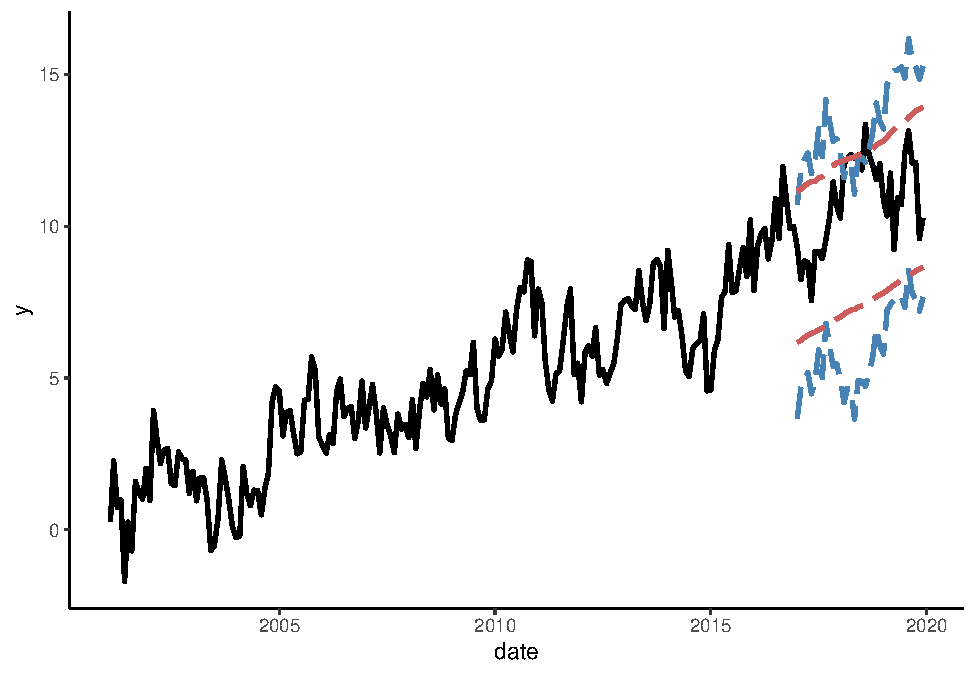
\includegraphics{forecasting_files/figure-latex/unnamed-chunk-105-1.pdf}

Test the unconditional coverage of the interval forecasts from the considered two models.

\begin{Shaded}
\begin{Highlighting}[]
\NormalTok{dt[,}\StringTok{\textasciigrave{}}\AttributeTok{:=}\StringTok{\textasciigrave{}}\NormalTok{(}\AttributeTok{i1=}\FunctionTok{ifelse}\NormalTok{(y}\SpecialCharTok{\textgreater{}=}\NormalTok{a1dl }\SpecialCharTok{\&}\NormalTok{ y}\SpecialCharTok{\textless{}=}\NormalTok{a1du,}\DecValTok{1}\NormalTok{,}\DecValTok{0}\NormalTok{),}\AttributeTok{it=}\FunctionTok{ifelse}\NormalTok{(y}\SpecialCharTok{\textgreater{}=}\NormalTok{trdl }\SpecialCharTok{\&}\NormalTok{ y}\SpecialCharTok{\textless{}=}\NormalTok{trdu,}\DecValTok{1}\NormalTok{,}\DecValTok{0}\NormalTok{))]}


\CommentTok{\# AR(1)}
\NormalTok{p1 }\OtherTok{\textless{}{-}} \FunctionTok{mean}\NormalTok{(dt}\SpecialCharTok{$}\NormalTok{i1,}\AttributeTok{na.rm=}\NormalTok{T)}

\NormalTok{L10 }\OtherTok{\textless{}{-}}\NormalTok{ (}\DecValTok{1}\FloatTok{{-}.95}\NormalTok{)}\SpecialCharTok{\^{}}\NormalTok{(P}\SpecialCharTok{*}\NormalTok{(}\DecValTok{1}\SpecialCharTok{{-}}\NormalTok{p1))}\SpecialCharTok{*}\NormalTok{(.}\DecValTok{95}\NormalTok{)}\SpecialCharTok{\^{}}\NormalTok{(P}\SpecialCharTok{*}\NormalTok{p1)}
\NormalTok{L11 }\OtherTok{\textless{}{-}}\NormalTok{ (}\DecValTok{1}\SpecialCharTok{{-}}\NormalTok{p1)}\SpecialCharTok{\^{}}\NormalTok{(P}\SpecialCharTok{*}\NormalTok{(}\DecValTok{1}\SpecialCharTok{{-}}\NormalTok{p1))}\SpecialCharTok{*}\NormalTok{(p1)}\SpecialCharTok{\^{}}\NormalTok{(P}\SpecialCharTok{*}\NormalTok{p1)}

\NormalTok{LR1 }\OtherTok{\textless{}{-}} \SpecialCharTok{{-}}\DecValTok{2}\SpecialCharTok{*}\FunctionTok{log}\NormalTok{(L10}\SpecialCharTok{/}\NormalTok{L11)}

\FunctionTok{pchisq}\NormalTok{(LR1,}\AttributeTok{df=}\DecValTok{1}\NormalTok{,}\AttributeTok{lower.tail=}\NormalTok{F)}
\end{Highlighting}
\end{Shaded}

\begin{verbatim}
## [1] 0.01027851
\end{verbatim}

\begin{Shaded}
\begin{Highlighting}[]
\CommentTok{\# AR(2)}
\NormalTok{p2 }\OtherTok{\textless{}{-}} \FunctionTok{mean}\NormalTok{(dt}\SpecialCharTok{$}\NormalTok{it,}\AttributeTok{na.rm=}\NormalTok{T)}

\NormalTok{L20 }\OtherTok{\textless{}{-}}\NormalTok{ (}\DecValTok{1}\FloatTok{{-}.95}\NormalTok{)}\SpecialCharTok{\^{}}\NormalTok{(P}\SpecialCharTok{*}\NormalTok{(}\DecValTok{1}\SpecialCharTok{{-}}\NormalTok{p2))}\SpecialCharTok{*}\NormalTok{(.}\DecValTok{95}\NormalTok{)}\SpecialCharTok{\^{}}\NormalTok{(P}\SpecialCharTok{*}\NormalTok{p2)}
\NormalTok{L21 }\OtherTok{\textless{}{-}}\NormalTok{ (}\DecValTok{1}\SpecialCharTok{{-}}\NormalTok{p2)}\SpecialCharTok{\^{}}\NormalTok{(P}\SpecialCharTok{*}\NormalTok{(}\DecValTok{1}\SpecialCharTok{{-}}\NormalTok{p2))}\SpecialCharTok{*}\NormalTok{(p2)}\SpecialCharTok{\^{}}\NormalTok{(P}\SpecialCharTok{*}\NormalTok{p2)}

\NormalTok{LR2 }\OtherTok{\textless{}{-}} \SpecialCharTok{{-}}\DecValTok{2}\SpecialCharTok{*}\FunctionTok{log}\NormalTok{(L20}\SpecialCharTok{/}\NormalTok{L21)}

\FunctionTok{pchisq}\NormalTok{(LR2,}\AttributeTok{df=}\DecValTok{1}\NormalTok{,}\AttributeTok{lower.tail=}\NormalTok{F)}
\end{Highlighting}
\end{Shaded}

\begin{verbatim}
## [1] 0.1441849
\end{verbatim}

\end{document}
